\documentclass[12pt,a4paper]{report}

\usepackage{alltt, fancyvrb, url}
\usepackage{graphicx}
\usepackage[utf8]{inputenc}
\usepackage{float}
\usepackage{xcolor}
\usepackage{hyperref}
\usepackage{longtable}
\usepackage{listings}
\usepackage{color}
\usepackage[utf8]{inputenc}

\usepackage{enumitem}
\usepackage{amsmath}
\usepackage{geometry}
\usepackage{pdfpages}

\geometry{margin=1in}

\definecolor{codegray}{rgb}{0.5,0.5,0.5}
\definecolor{codepurple}{rgb}{0.58,0,0.82}
\definecolor{backcolour}{rgb}{0.95,0.95,0.92}

\lstdefinestyle{sqlstyle}{
    language=SQL,
    backgroundcolor=\color{backcolour},
    commentstyle=\color{codegreen},
    keywordstyle=\color{codepurple},
    numberstyle=\numberstyle,
    stringstyle=\color{codepurple},
    basicstyle=\footnotesize\ttfamily,
    breakatwhitespace=false,
    breaklines=true,
    captionpos=b,
    keepspaces=true,
    numbers=left,
    numbersep=10pt,
    showspaces=false,
    showstringspaces=false,
    showtabs=false
}
\newcommand\numberstyle[1]{%
    \footnotesize
    \color{codegray}%
    \ttfamily
    \ifnum#1<10 0\fi#1 |%
}

\usepackage{newlfont}
\usepackage{gensymb}

\usepackage[italian]{babel}
\usepackage[capitalise, italian]{cleveref}

\graphicspath{ {./src/img} }

\textwidth=450pt\oddsidemargin=0pt
\begin{document}

\begin{titlepage}
\begin{center}
{{\Large{\textsc{Alma Mater Studiorum $\cdot$ Università di Bologna}}}} \rule[0.1cm]{15.8cm}{0.1mm}
\rule[0.5cm]{15.8cm}{0.6mm}
{\small{\bf CORSO DI LAUREA IN INGEGNERIA E SCIENZE INFORMATICHE \\ A.A. 2024/25 }}
\end{center}
\vspace{15mm}
\begin{center}
{\LARGE{\bf Smart City - Mobilità Integrata}}
\end{center}
\begin{center}
{\LARGE Relazione per il corso di Basi di Dati }
\end{center}

\vspace{8mm}
\begin{center}
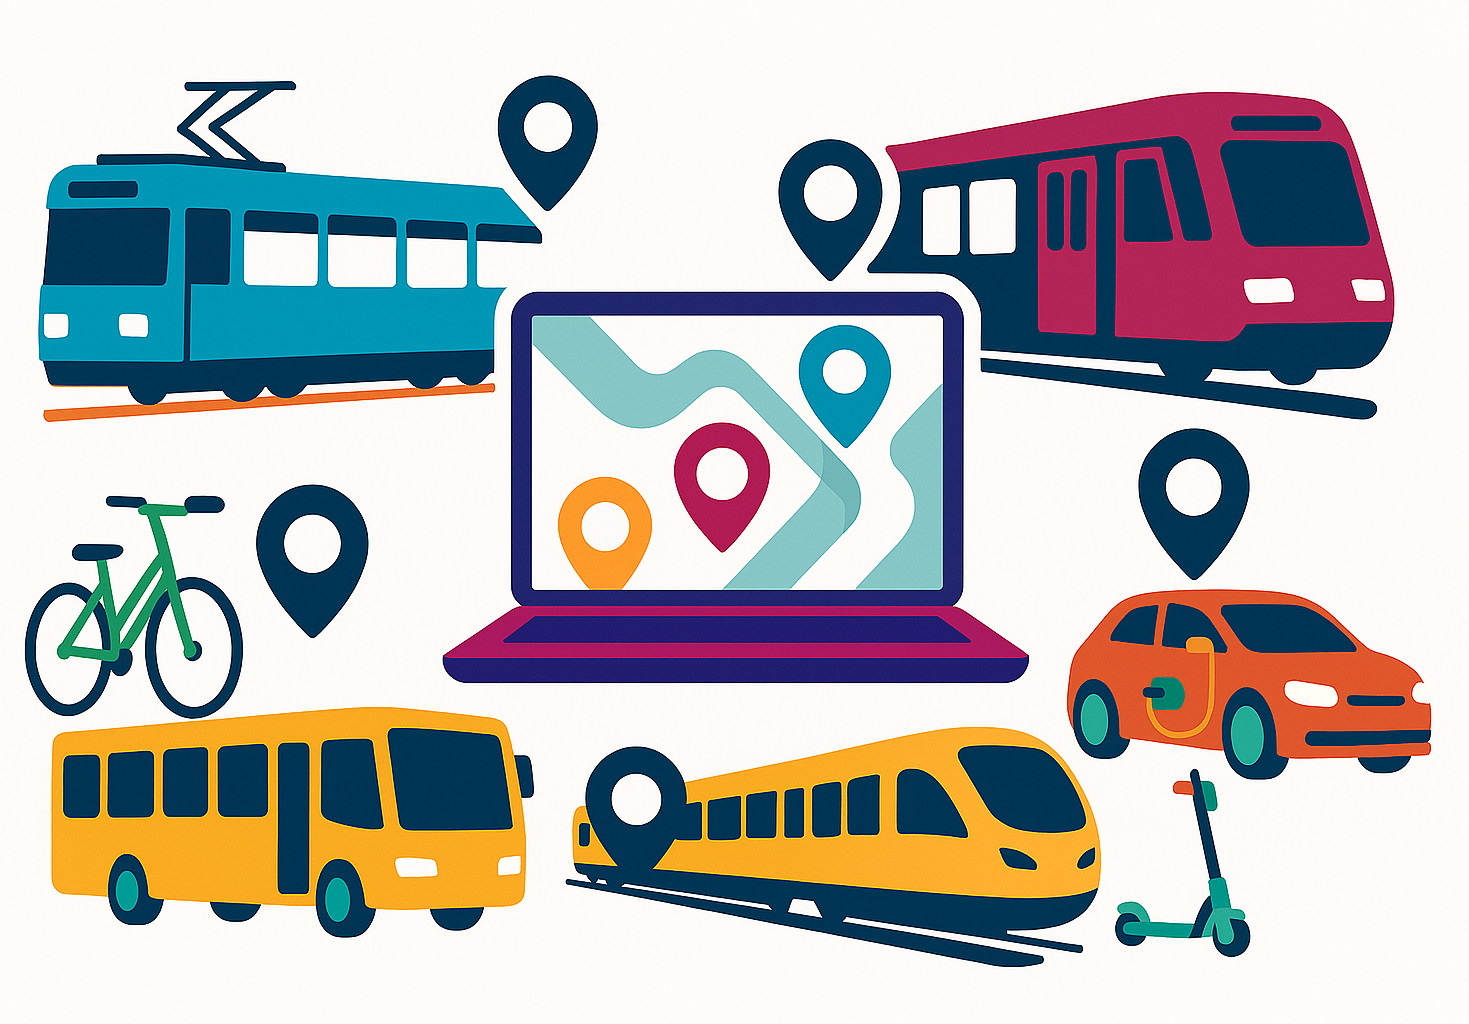
\includegraphics[width=0.8\textwidth]{Copertina}
\end{center}
\vspace{10mm}

{\large{\bf \noindent
Componenti del gruppo nr.2743:\\}
Bartocetti Enrico, matr. 0001115097\\
Benedetti Nicholas, matr. 0001114021\\
Tazzieri Nicolas, matr. 0001114078}

\end{titlepage}

\tableofcontents


\chapter{Analisi dei requisiti}

\section{Intervista iniziale}
Si vuole realizzare il software per la gestione del trasporto pubblico a lungo e corto raggio.
A seguito dell’intervista è stata prodotta la seguente descrizione delle specifiche del sistema in linguaggio naturale:
\\ \\
\textit{Le città di Vergineto, Urbania e San Giovanni in Marignano si sono accordate per avviare il progetto “Smart mobility 2030”, e richiedono un software per la gestione Smart e integrata del trasporto pubblico urbano ed extraurbano.}

\textit{Il sistema dovrà gestire diversi mezzi di TPL (Trasporto Pubblico Locale), quali bus, tram, metropolitana e treni ma in futuro potrebbe sorgere la necessità di aggiungerne di nuovi (ad esempio in seguito alla creazione di linee per i filobus). Ogni mezzo potrà percorrere diverse linee: ciò significa che un autobus utilizzato oggi per la linea 15, domani potrà percorrere la linea 21.}

\textit{Per ogni linea verranno effettuate delle fermate a orari prestabiliti. Potranno essere create anche linee straordinarie, ad esempio delle navette per eventi cittadini, di cui dovranno essere specificati periodo di validità, orari e fermate.}

\textit{Inoltre, per ridurre l’inquinamento nelle nostre città, verranno creati degli spazi riservati per lo sharing di biciclette, scooter e biciclette, e verranno aggiunte delle colonnine per la ricarica elettrica in modo da incentivare sia l’acquisto di auto elettriche sia l’utilizzo di monopattini o bici elettriche.}

\textit{Sarà disponibile una piattaforma online, nella quale si potranno visualizzare le diverse linee e le fermate che i mezzi effettuano con i relativi orari, nonché la disponibilità di posti liberi nelle aree di bikesharing e nelle colonnine elettriche. È anche prevista la registrazione di utenti “cittadini”, che potranno acquistare biglietti e abbonamenti. }

\textit{Un unico biglietto vale per tutti i mezzi di trasporto, e si vuole memorizzarne la durata, la data di convalida, la data di acquisto ed il titolare nel caso venga acquistato online: infatti un biglietto potrà anche essere acquistato da un fornitore fisico (ad esempio le tabaccherie della città). Sono presenti diverse tipologie di biglietti che differiscono in base alla durata dalla convalida e al prezzo. Gli abbonamenti sono biglietti che hanno una durata superiore ad un giorno.}

\textit{Si richiede anche la gestione dei dipendenti. In particolare, dovranno essere gestiti diversi autisti a cui verranno assegnati diversi mezzi in diversi slot orari. Sono inoltre presenti i controllori: in certi orari dovranno controllare diverse linee e saranno in grado di emettere multe. Gli orari e le linee da controllare vengono stabilite dal gestore delle linee di trasporto: ad esempio verranno prese in particolare considerazione quelle dove non ci sono molti incassi, ovvero dove è ipotizzabile una maggior evasione tariffaria, generando ingenti perdite economiche. Infine, l’amministratore del sistema potrà registrarsi in un portale specifico nel quale potrà gestire autisti, controllori e le linee. Inoltre, avrà la possibilità di visualizzare diverse statistiche riguardanti il sistema di trasporto, con enfasi particolare nei ricavi dei biglietti e nel tasso di evasione.}

\textit{Dovranno essere gestiti i lavori di manutenzione relativi a linee e mezzi per cui saranno specificati gli eventuali enti privati che li svolgeranno. Per le manutenzioni sarà richiesto di specificare una data di inizio e fine lavori, ed eventuali variazioni di servizio dovranno essere visualizzate al pubblico.}


\section{Prima fase di analisi}
Nell’analisi dell’intervista effettuata tempo addietro, abbiamo notato che il committente non è stato abbastanza esaustivo su alcuni argomenti.
Si è quindi resa necessaria un’ulteriore intervista per comprendere meglio il funzionamento di:
\begin{itemize}
	\item Sistema di acquisto e convalida di biglietti
	\item Gestione degli spazi speciali
	\item Gestione delle multe
\end{itemize}
\noindent Riportiamo le risposte R alle varie domande D.

\paragraph{D:}
“Come devono essere gestiti i biglietti, dal loro acquisto fino alla convalida?”
\\ {\bf R:} “I biglietti possono essere acquistati tramite il sito web, le biglietterie fisiche (sia dell’azienda sia da altri venditori autorizzati) e ticketmachine.
Ogni mezzo sarà dotato di una obliteratrice che, comunicando con il sistema informativo, alla lettura di un biglietto (tramite codice a barre stampato sul biglietto fisico o letto dal proprio dispositivo) ne controlla la validità e in caso affermativo lo registra come convalidato.”

\paragraph{D:}
“Cosa deve essere mostrato riguardo agli spazi per la mobilità sostenibile?”
\\ {\bf R:} “L’idea è quella di far vedere giusto una panoramica riguardo agli spazi.
In particolare, basta visualizzarne la posizione, l’indirizzo, un nome simbolico e quanti sono i posti rimanenti (quante biciclette rimanenti se si tratta di biciclette, quante colonnine se si tratta di colonnine elettriche, ecc.).
Inoltre, uno spazio può essere legato ad una fermata per rendere agevole il collegamento con aree non raggiunte dalle linee del TPL (es. appena scendo dal bus mi trovo nei pressi di una zona per il bike sharing)”

\paragraph{D:}
“Come funziona il sistema delle multe?”
\\ {\bf R:} “Le multe possono essere emesse dal personale qualificato a seguito di controlli effettuati sulle linee.
A ogni causale della multa corrisponde un certo importo base, e un importo massimo. Il controllore potrà assegnare un importo che sia compreso tra questi due valori”


\section{Concetti principali}
Per rendere meglio fruibile la descrizione, abbiamo deciso di rimuovere eventuali ambiguità, seguendo la tabella qua sotto.

\begin{table}[h!]
\begin{tabular}{|l|l|}
\hline
\textbf{Termine} & \textbf{Nuovo Termine} \\
\hline
Mezzi di TPL & Mezzi di trasporto \\
Spazi riservati per il carsharing, … & Hub mobilità \\
Biglietti, Abbonamenti & Titolo di Viaggio \\
Gestore delle linee & Amministratore di Sistema \\
\hline
\end{tabular}
\end{table}

A seguito dell’intervista aggiuntiva è stata redatta la seguente descrizione del dominio in linguaggio naturale. Ambiguità e informazioni ridondanti sono state eliminate per garantire una miglior fruizione della descrizione:
\\ \\
Le città di Vergineto, Urbania e San Giovanni in Marignano si sono accordate per avviare il progetto “Smart mobility 2030”, e richiedono un software per la gestione Smart e integrata del trasporto pubblico urbano ed extraurbano.

Il sistema dovrà gestire diversi \underline{\texttt{mezzi di trasporto}}, quali \underline{\texttt{bus}}, \underline{\texttt{tram}}, \underline{\texttt{metropolitana}} e \underline{\texttt{treni}} lasciando la possibilità di aggiungerne altri in futuro. Ogni mezzo di trasporto potrà percorrere diverse \underline{\texttt{linee}}.

Una linea può essere \underline{\texttt{ordinaria}} o \underline{\texttt{straordinaria}}. Ogni linea effettua \underline{\texttt{fermate}} ad \underline{\texttt{orari}} prestabiliti. Per una linea straordinaria dovrà essere specificato il periodo di validità della linea.

Dovranno essere gestiti degli \underline{\texttt{hub mobilità}}, riservati per la ricarica elettrica e lo sharing di bici, monopattini e scooter. In particolare, si devono memorizzare la posizione, l’indirizzo, un nome simbolico e quanti sono i posti rimanenti. Inoltre, ad un hub mobilità può essere \underline{\texttt{associato}} ad una fermata.

Sarà disponibile una piattaforma online, nella quale si potranno visualizzare le diverse linee e le fermate che i mezzi effettuano con i relativi orari, nonché la disponibilità di posti liberi negli hub mobilità. È anche prevista la registrazione di \underline{\texttt{utenti cittadini}}, che potranno \underline{\texttt{acquistare}} \underline{\texttt{titoli di viaggio}}, che si dividono in \underline{\texttt{biglietti}} e \underline{\texttt{abbonamenti}}.

Un unico titolo di viaggio vale per tutti i mezzi di trasporto e vuole memorizzarne la durata, la data di convalida, la data di acquisto e l’utente cittadino associato nel caso sia un \underline{\texttt{biglietto digitale}}. Sono presenti diverse \underline{\texttt{tipologie}} di titoli di viaggio che differiscono in base alla durata dalla convalida e al prezzo. Gli abbonamenti sono biglietti che hanno una durata superiore ad un giorno. I biglietti possono essere acquistati anche in biglietterie fisiche e ticketmachine. Ogni mezzo di trasporto sarà dotato di una obliteratrice che, comunicando con il sistema informativo, alla lettura di un biglietto ne controlla la validità, e in caso affermativo, lo registra come \underline{\texttt{convalidato}}.

Si richiede anche la gestione dei \underline{\texttt{dipendenti}}. Essi si dividono in \underline{\texttt{Autisti}}, \underline{\texttt{Controllori}} e \underline{\texttt{Amministratori di sistema}}. Agli Autisti a verranno assegnati diversi mezzi di trasposto in slot orari diversi. I controllori dovranno controllare diverse linee negli slot orari assegnati, e saranno in grado di emettere \underline{\texttt{multe}}.  A ogni \underline{\texttt{causale della multa}} corrisponde un certo importo base e uno massimo. Il controllore potrà assegnare un importo alla multa tra questi due valori. Gli orari e le linee da controllare vengono stabilite dall’amministratore di sistema. Infine, l’amministratore del sistema potrà registrarsi in un portale specifico nel quale potrà gestire autisti, controllori e le linee. Inoltre, avrà la possibilità di visualizzare diverse statistiche riguardanti il sistema di trasporto, con enfasi particolare nei ricavi dei titoli di viaggio e nel tasso di evasione.

Dovranno essere gestiti i lavori di \underline{\texttt{manutenzione}}, che possono coinvolgere \underline{\texttt{linee}} e \underline{\texttt{mezzi di trasporto}}, per cui saranno specificati gli eventuali \underline{\texttt{enti privati}} che li svolgeranno. Per le manutenzioni sarà richiesto di specificare una data di inizio e fine lavori, ed eventuali \underline{\texttt{variazioni di servizio}} che coinvolgono linee dovranno essere visualizzate al pubblico.

\chapter{Progettazione Concettuale}
In questo capitolo mostreremo la realizzazione dello schema ER. Partiamo da uno schema scheletro per poi, attraverso degli step di raffinamento, arrivare allo schema finale mantenendo un approccio top-down.
\section{Schema Scheletro}
In seguito all'analisi del dominio abbiamo realizzato lo schema scheletro, contenente le principali entità e associazioni che andremo a raffinare nei prossimi step.\\

\begin{centering}
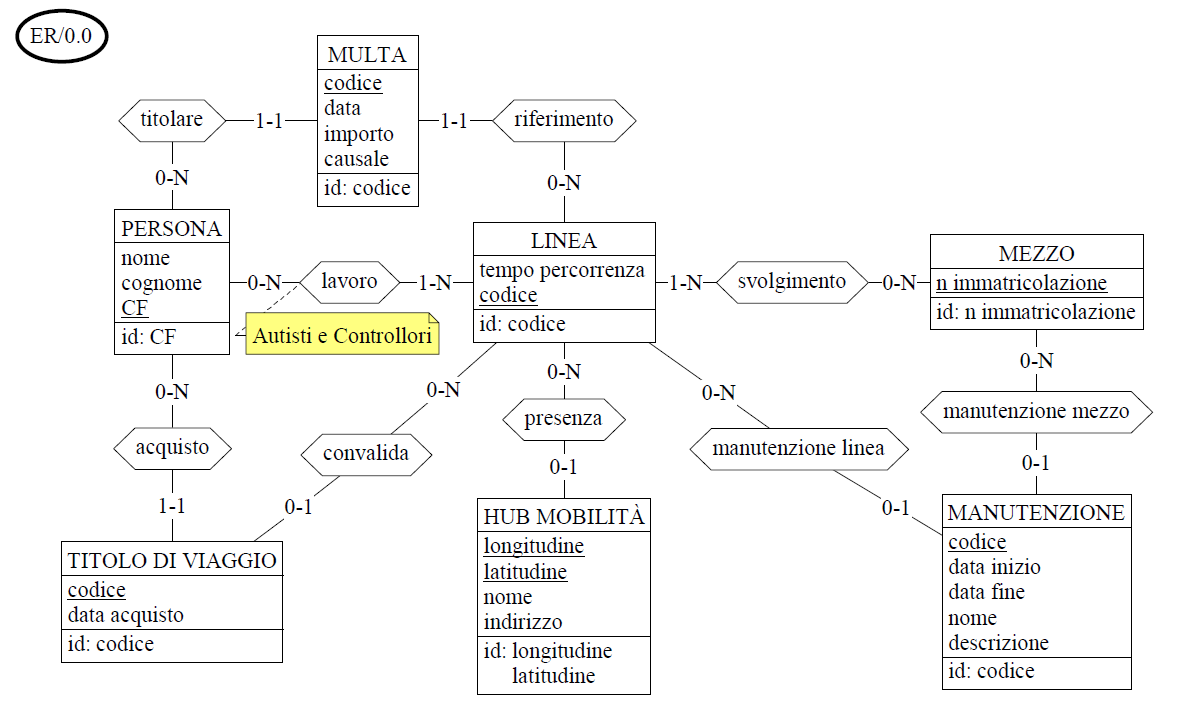
\includegraphics[width=1.0\textwidth]{prog_conc/Scheletro}
\end{centering}

\section{Raffinamenti Proposti}

\subsection{Linee e Hub mobilità}
Per modellare le linee abbiamo creato una gerarchia totale ed esclusiva formata da due entità una rappresentante le linee ordinarie, una le linee straordinarie. Per modellare le varie tipologie di mezzi che possono operare in una linea abbiamo aggiunto l'entità \texttt{TIPOLOGIA MEZZO}. L'entità \texttt{TRATTA} modella l'esistenza di un percorso tra due fermate e ne memorizza il tempo di percorrenza. Una linea verrà quindi intesa come sequenza ordinata di tratte attraverso l'associazione \texttt{TRAGITTO}. Per gestire le varie tipologie di contenuti negli hub abbiamo creato l'entità \texttt{CONTENUTO HUB}: associata a uno specifico \texttt{HUB MOBILITA} ne memorizza il numero di posti massimi e quelli disponibili. Siccome non ci interessa storicizzare l'utilizzo degli hub mobilità, posti disponibili rimane un attributo dell'associazione contenuto che verrà incrementato / decrementato all'occorrenza (sempre rispettando il limite 0  {\textless}= disponibili {\textless}= massimi). Infine per modellare l'eventuale presenza di una fermata vicino ad un hub abbiamo creato l'associazione opzionale \texttt{presenza}.
Con questa modellazione rimangono dei vincoli inespressi da gestire, la cui discussione viene effettuata nella \cref{section:VincoliInespressi}.\\
\begin{centering}
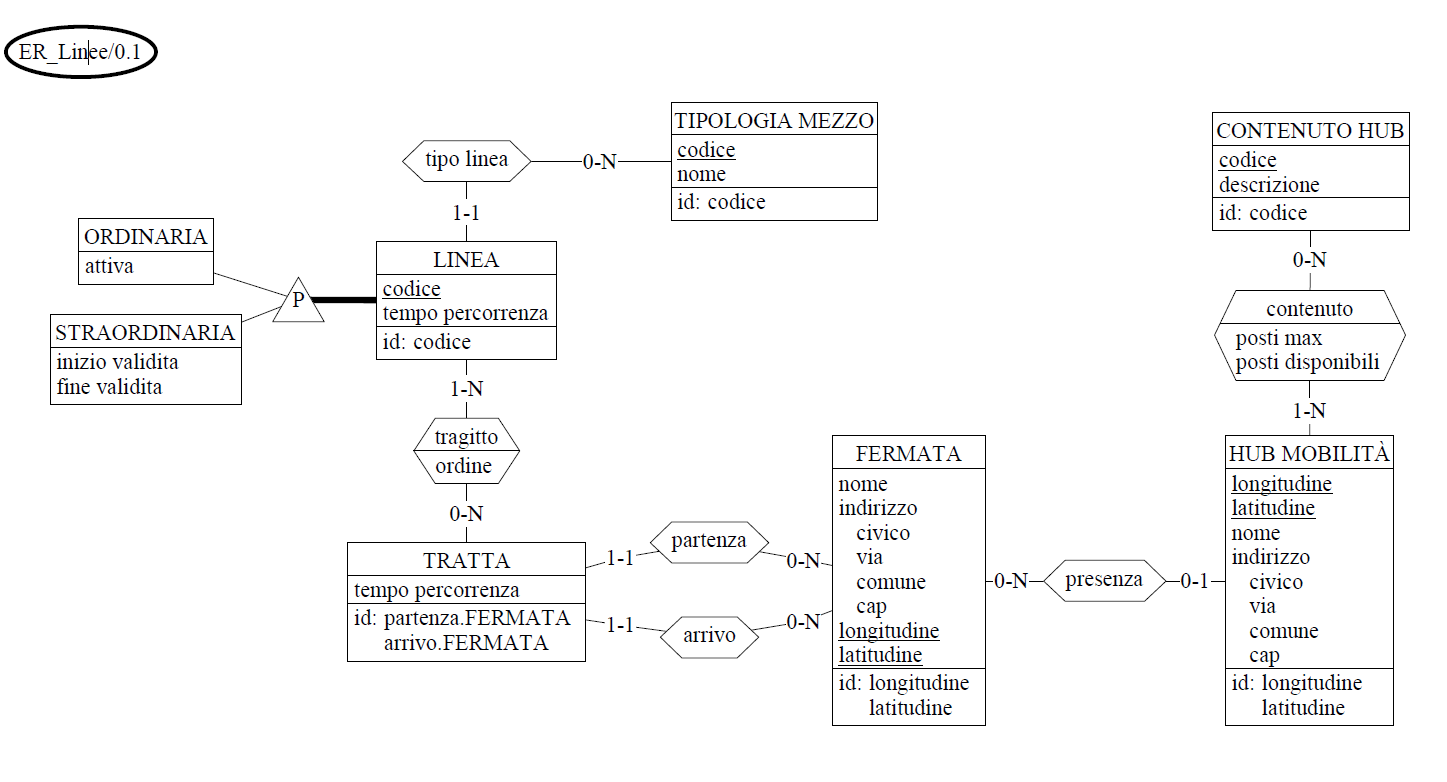
\includegraphics[width=1.0\textwidth]{prog_conc/Linee}
\end{centering}

\subsection{Manutenzioni}
Nel nostro dominio gli oggetti delle manutenzioni possono essere sia le \texttt{LINEE} che i \texttt{MEZZI}: per questo abbiamo raccolto gli attributi comuni nell'entità \texttt{MANUTENZIONE} e poi creato una gerarchia totale ed esclusiva per diversificare mezzi e linee.
Visto che una manutenzione può essere svolta sia internamente sia affidandola a un'\texttt{AZIENDA} terza, abbiamo inserito un'associazione opzionale tra la manutenzione e l'azienda. \\
Per ridurre al minimo i disservizi, per ogni linea \texttt{ORDINARIA} posta in manutenzione si possono prevedere una serie di linee \texttt{STRAORDINARIE} che la rimpiazzano. \\
\begin{centering}
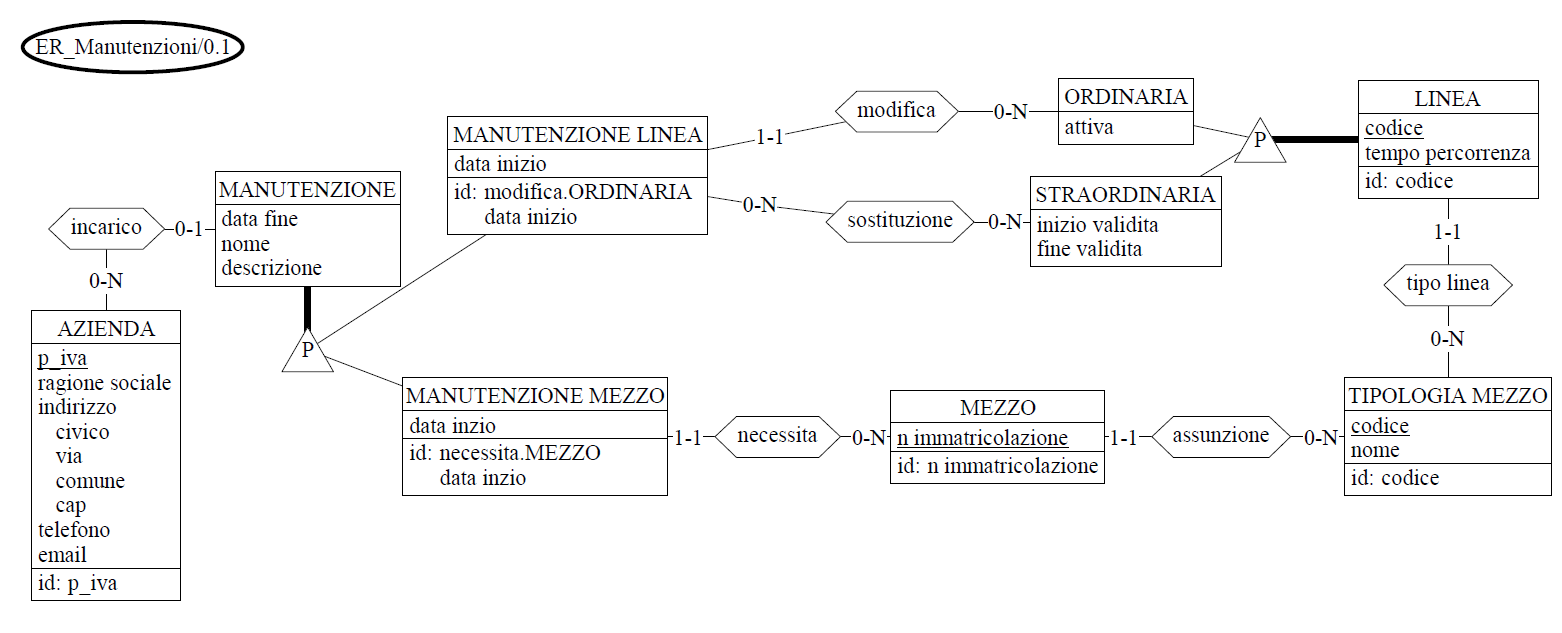
\includegraphics[width=1.0\textwidth]{prog_conc/Manutenzioni}
\end{centering}

\subsection{Persone}
Per la modellazione delle persone abbiamo deciso di creare diversi livelli di gerarchia:
\begin{itemize}
  \item Persone: Raccoglie i dati anagrafici di una persona
  \item Utenti: Subset di \texttt{PERSONA} registrate al sistema con username e password
  \item Dipendenti: Subset di \texttt{UTENTE} che lavorano al alla azienda TPL
  \item Controllori-Autisti-Amministrativi: Gerarchia totale ed esclusiva per specificare il ruolo del \texttt{DIPENDENTE} all'interno dell'azienda
\end{itemize}
Grazie a questa modellazione evidenziamo che il controllore potrà controllare alcune linee e un autista potrà condurre diverse linee. Questa modellazione non è ottimale poiché manca sia uno storico delle corse e controlli svolti, sia perché non è chiaro quando questi andranno effettuati: nei prossimi step andremo a risolvere il problema della storicizzazione, così da modellare anche un orario di lavoro.
Per quanto riguarda le multe, è stata creata l'entità \texttt{MULTA} associata al controllore che la emette, alla linea nella quale è stata commessa l'infrazione e alla persona che ha commesso il reato. Per gestire l'importo della multa è stata creata l'entità \texttt{CAUSALE MULTA} che dato un tipo di infrazione viene determinato un prezzo base e prezzo massimo alla multa (il cui importo sarà deciso a discrezione del controllore). \\
\begin{centering}
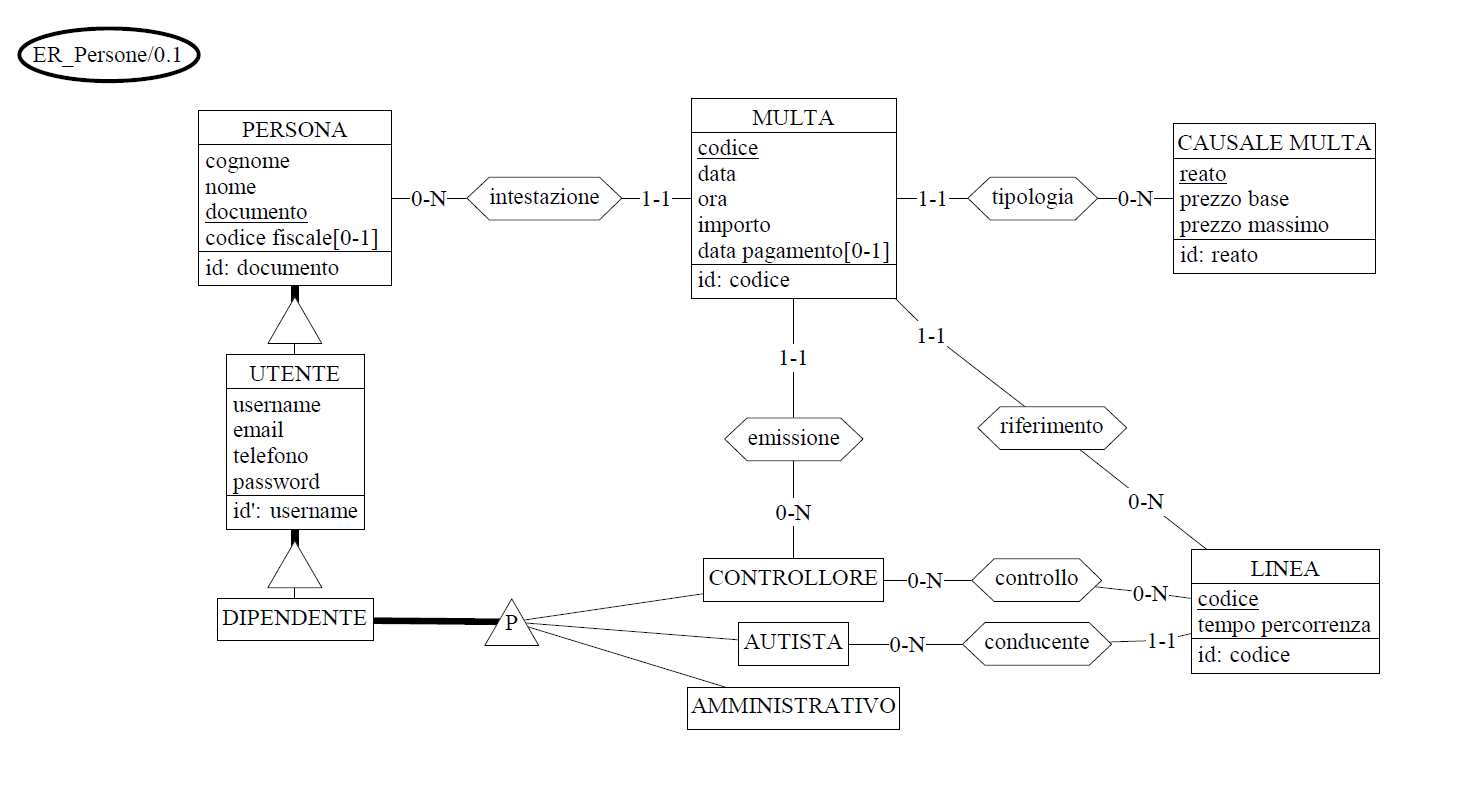
\includegraphics[width=1.0\textwidth]{prog_conc/Persone}
\end{centering}

\subsection{Orari Linee e mezzi}
Per la gestione degli orari delle linee abbiamo aggiunto un'entità \texttt{ORARIO LINEA} i cui attributi (giorno ed ora) fanno tutti parte della chiave. In questo modo per ogni linea si può specificare un giorno settimanale e più orari di partenza per lo stesso giorno. Per storicizzare le corse abbiamo aggiunto \texttt{ATTUAZIONE CORSA} che fa riferimento ad un orario di una linea effettuato in una certa data, da un certo autista, tramite uno specifico mezzo e su cui possono essere assegnati vari controllori (le cui multe saranno associate alla corsa su cui sono state emesse). Va però controllato che il giorno settimanale della data sia lo stesso di quello associato a \texttt{ORARIO LINEA}.
In questa maniera è stato possibile modellare l'orario di lavoro dei dipenenti, che farà riferimento ad una specifica \texttt{ATTUAZIONE CORSA}. Un altro vincolo inespresso da rispettare è che la tipologia del mezzo associato all'attuazione corsa deve essere la stessa associata alla linea.\\
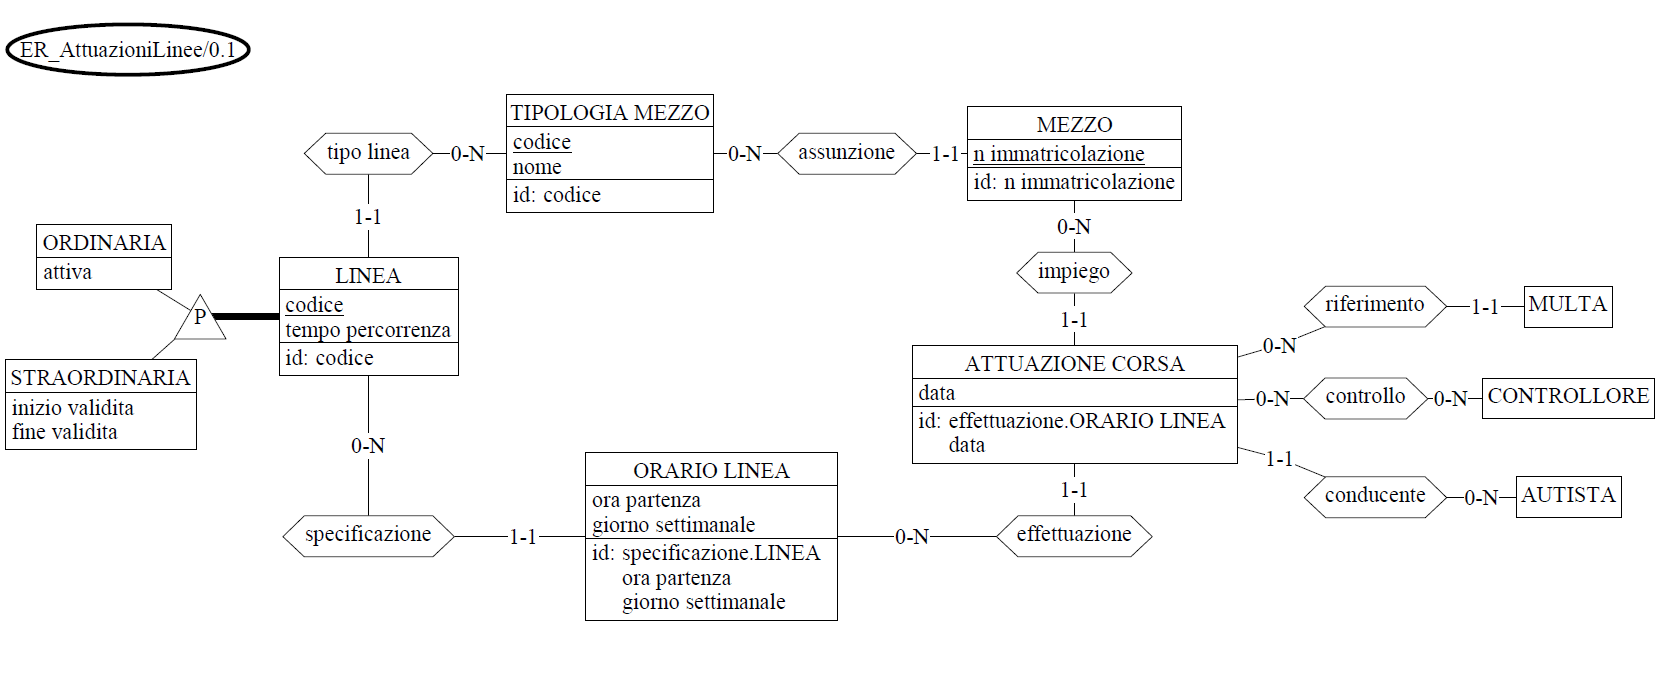
\includegraphics[width=1.0\textwidth]{prog_conc/AttuazioniLinee}

\subsection{Titolo di Viaggio}
Per quanto riguarda la gestione dei titoli di viaggio, come da requisiti, abbiamo generalizzato il concetto e creato due sottoentità \texttt{BIGLIETTO} e \texttt{ABBONAMENTO}. Un abbonamento è sempre associato all'utente proprietario del titolo. Per quanto riguarda i tariffari abbiamo creato due entità separate: per i biglietti la durata in minuti definisce il nome e il prezzo, mentre per gli abbonamenti è il numero di giorni di validità a determinarli. Anche il concetto di biglietto è stato generalizzato, creando le sottoentità \texttt{BIGLIETTO FISICO} e \texttt{BIGLIETTO DIGITALE}; quest'ultimo è sempre associato all'utente proprietario del biglietto. Per gestire le convalide abbiamo aggiunto l'associazione opzionale \texttt{convalida} con un'attuazione corsa che contiene la data e l'ora della convalida. In questa maniera sarà possibile tenere traccia delle linee in cui verranno effettuate più convalide.
\\
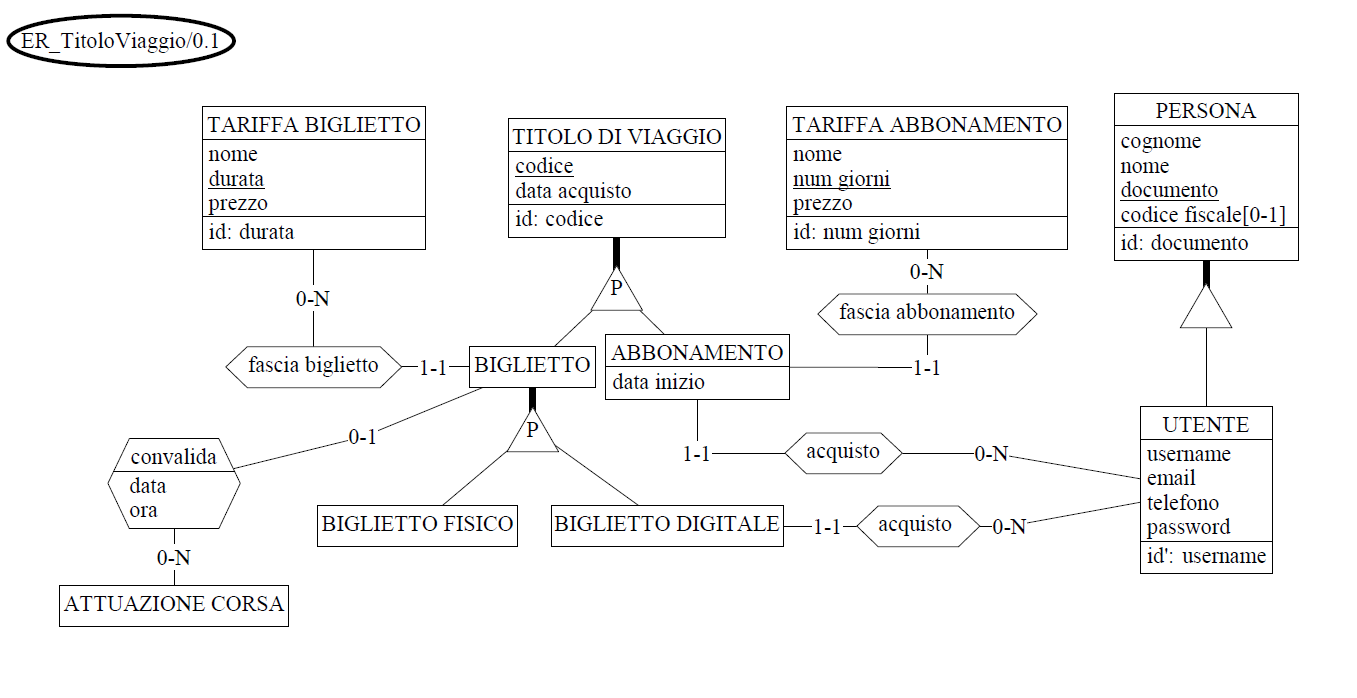
\includegraphics[width=1.0\textwidth]{prog_conc/TitoliViaggio}

\section{Schema Concettuale Finale}
Nella pagina seguente è presente lo schema concettuale finale completo.
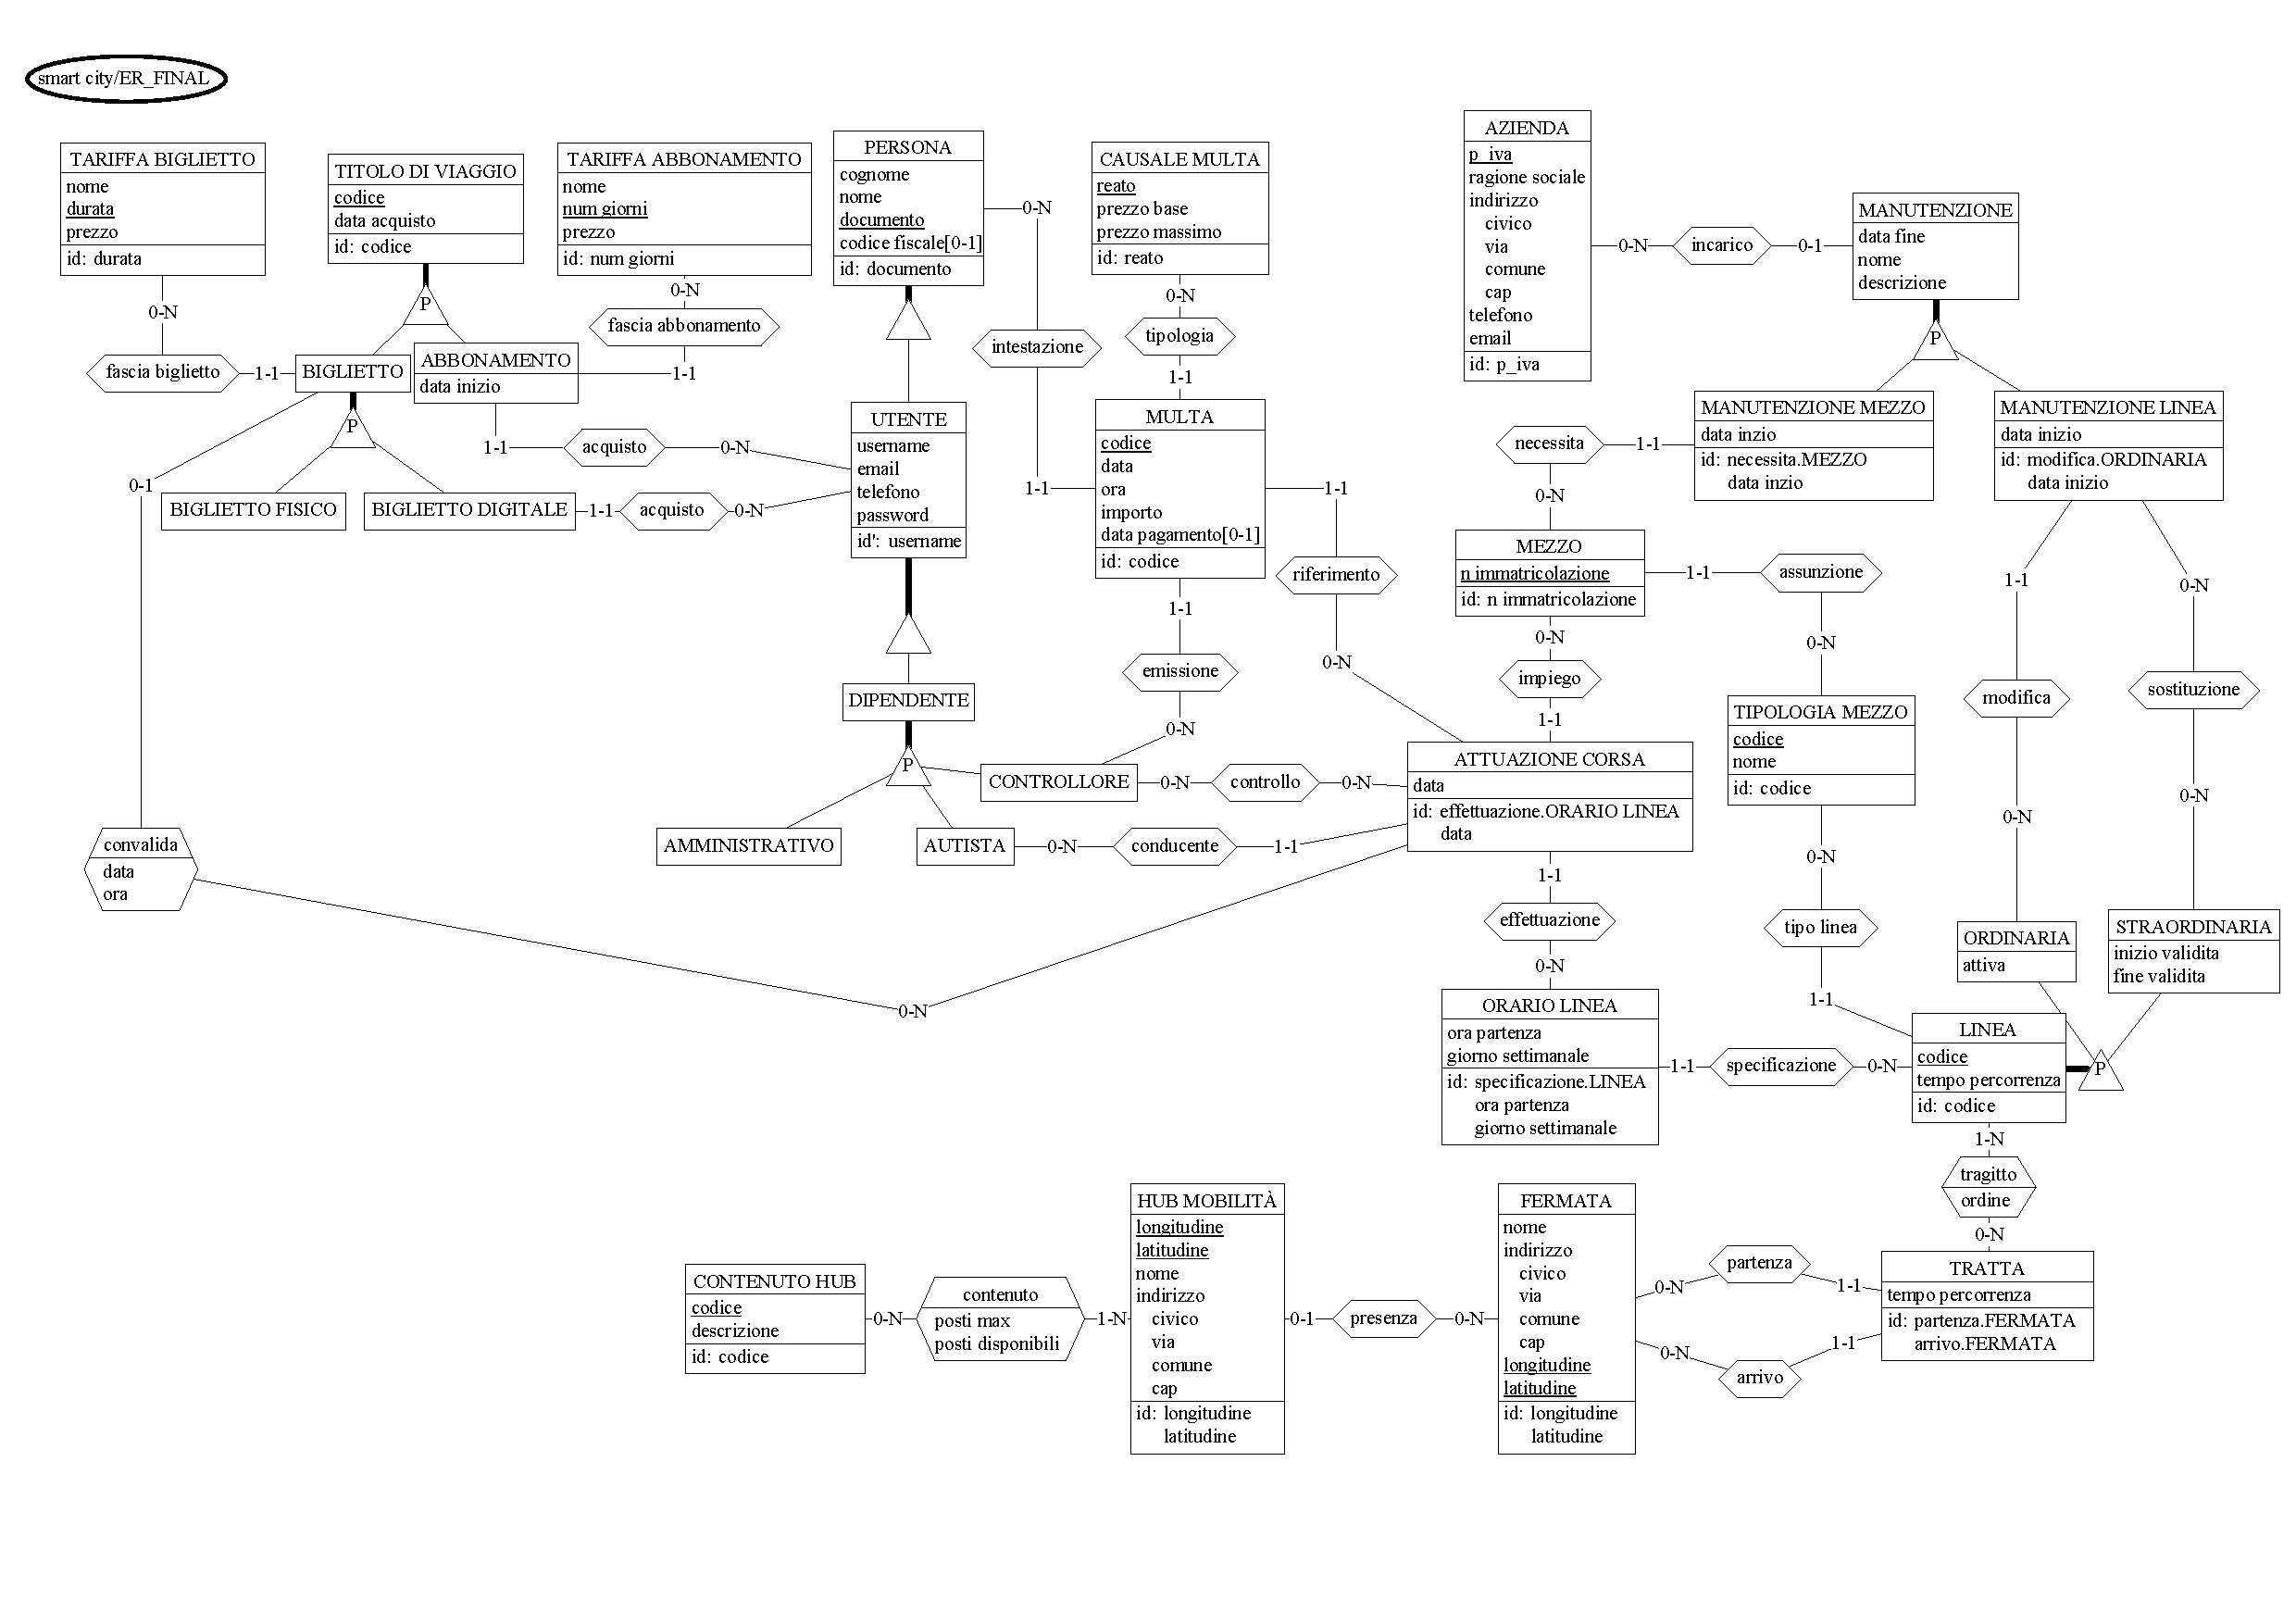
\includepdf{src/pdf/Schema_ER.pdf}

\subsection{Vincoli inespressi}\label{section:VincoliInespressi}

In questa sezione discuteremo i vari vincoli inespressi dal nostro schema concettuale:
\begin{itemize}
  \item In un \texttt{TRAGITTO} la tratta $n$-esima deve avere la fermata di partenza che coincide con la fermata di arrivo della tratta ($n-1)$-esima
  \item In una \texttt{TRATTA} le fermate di partenza e arrivo devono essere diverse
  \item In \texttt{CONTENUTO} \texttt{posti\_max} $ \geq $ \texttt{posti\_disponibili}
  \item In \texttt{CAUSALE\_MULTA} \texttt{prezzo\_base} $ \leq $ \texttt{prezzo\_massimo}
  \item In \texttt{ATTUAZIONE\_CORSA} il giorno settimanale della data deve coincidere con il giorno settimanale in \texttt{ORARIO\_LINEA}
  \item Il mezzo assegnato a un'\texttt{ATTUAZIONE\_CORSA} deve avere la stessa \texttt{TIPOLOGIA\_MEZZO} assegnata alla \texttt{LINEA} di riferimento
  \item Nell'aggiunta di un \texttt{AUTISTA} a un'\texttt{ATTUAZIONE\_CORSA} bisogna controllare che durante tutta la durata della corsa l'autista non sia già stato assegnato ad altre linee (ovvero che non si sovrapponga l'orario di lavoro)
\end{itemize}

\chapter{Progettazione Logica}
\section{Stima del volume dei dati}
Per poter gestire al meglio il carico di lavoro della base di dati, insieme al committente si è creata una stima del volume dei dati per entità e associazioni che il database dovrà gestire, di cui se ne riportano i numeri nella Tabella \ref{table:volumeDati}.
La stima è valida per un carico di lavoro di circa 6 mesi.

\begin{longtable}{|p{7.5cm}|r|c|}
\caption{Stima del volume dei dati}
\label{table:volumeDati}\\
\hline
\textbf{NOME} & \textbf{VOLUME STIMATO} & \textbf{E/A} \\
\hline
\endhead

ABBONAMENTO & 30.000 & E \\
\hline
AMMINISTRATIVO & 10 & E \\
\hline
ATTUAZIONE CORSA & 250.000 & E \\
\hline
AUMENTO & 10 & E \\
\hline
AUTISTA & 130 & E \\
\hline
AZIENDA & 15 & E\\
\hline
BIGLIETTO DIGITALE & 150.000 & E \\
\hline
BIGLIETTO FISICO & 150.000 & E \\
\hline
CAUSALE MULTA & 10 & E \\
\hline
CONTENUTO HUB & 4 & E \\
\hline
CONTROLLORE & 40 & E \\
\hline
DIPENDENTE & 180 & E \\
\hline
FERMATA & 450 & E \\
\hline
HUB MOBILITÀ & 225 & E \\
\hline
LINEA & 75 & E \\
\hline
MANUTENZIONE & 50 & E \\
\hline
MANUTENZIONE LINEA & 10 & E \\
\hline
MANUTENZIONE MEZZO & 40 & E \\
\hline
MEZZO & 160 & E \\
\hline
MULTA & 10.000 & E \\
\hline
ORARIO LINEA & 1500 & E \\
\hline
ORDINARIA & 65 & E \\
\hline
PERSONA & 20.000 & E \\
\hline
STRAORDINARIA & 10 & E \\
\hline
TARIFFA ABBONAMENTO & 5 & E \\
\hline
TARIFFA BIGLIETTO & 10 & E \\
\hline
TIPOLOGIA MEZZO & 4 & E \\
\hline
TITOLO DI VIAGGIO & 750.000 & E \\
\hline
TRATTA & 1.000 & E \\
\hline
UTENTE & 10.000 & E \\
\hline
ACQUISTO ABBONAMENTO & 30.000 & A \\
\hline
ACQUISTO BIGLIETTO & 150.000 & A \\
\hline
ARRIVO & 1.000 & A \\
\hline
ASSUNZIONE & 160 & A \\
\hline
CONDUCENTE & 250.000 & A \\
\hline
CONTENUTO & 450 & A \\
\hline
CONTROLLO & 50.000 & A \\
\hline
CONVALIDA & 200.000 & A \\
\hline
EFFETTUAZIONE & 250.000 & A \\
\hline
EMISSIONE & 10.000 & A \\
\hline
FASCIA ABBONAMENTO & 30.000 & A \\
\hline
FASCIA BIGLIETTO & 300.000 & A \\
\hline
IMPIEGO & 250.000 & A \\
\hline
INCARICO & 25 & A \\
\hline
INCREMENTO & 10 & A \\
\hline
INTESTAZIONE & 10.000 & A \\
\hline
MODIFICA & 10 & A \\
\hline
NECESSITA & 40 & A \\
\hline
PARTENZA & 1.000 & A \\
\hline
PRESENZA & 165 & A \\
\hline
RIFERIMENTO & 10.000 & A \\
\hline
SOSTITUZIONE & 10 & A \\
\hline
SPECIFICAZIONE & 1.500 & A \\
\hline
TIPO LINEA & 75 & A \\
\hline
TIPOLOGIA & 10.000 & A \\
\hline
TRAGITTO & 1.500 & A \\
\hline
\end{longtable}


\section{Descrizione operazioni}
Riportiamo in Tabella \ref{table:operazioni} le principali operazioni che saranno svolte sulla base di dati, marcando con un asterisco (*) le operazioni di cui è necessario calcolare i costi dati da attributi ridondanti.

\begin{longtable}{|c|p{9cm}|c|l|l|}
\caption{Numero stimato di operazioni per settimana, con tipo di utente che le effettua}
\label{table:operazioni}\\
\hline
\textbf{\#} & \textbf{Operazione} & \textbf{Op / 7gg} & \textbf{Tipo Utente} \\
\hline
\endhead
1*  & \hyperref[op1]{Visualizzazione di tutte le linee attive} & 4.000 & Tutti **** \\
\hline
2 & \hyperref[op2]{Visualizzazione fermate e orari di una linea} & 3.500 & Tutti **** \\
\hline
3 & \hyperref[op3]{Visualizzazione degli hub mobilità} & 500 & Tutti \\
\hline
4* & \hyperref[op4]{Visualizzazione orario e mezzo assegnato} & 150 & Autista ***** \\
\hline
5* & \hyperref[op5]{Visualizzazione orario e linee assegnate} & 100 & Controllore ***** \\
\hline
6 & \hyperref[op6]{Estrazione delle linee con più convalide nell'ultimo mese} & 3 & Amministratore *****  \\
\hline
7 & \hyperref[op7]{Estrazione delle manuntenzioni che coinvolgono un determinato mezzo} & 5 & Amministratore \\
\hline
8 & \hyperref[op8]{Estrazione delle manuntenzioni ed eventuali linee sostitutive che coinvolgono una linea} & 5 & Amministratore ***** \\
\hline
9 & \hyperref[op9]{Visualizzazione incassi dati dalle convalide per una linea} & 10 & Amministratore **** \\
\hline
10 & \hyperref[op10]{Estrazione degli incassi per tipo di titolo in periodo definito} & 5 & Amministratore \\
\hline
11 & \hyperref[op11]{Estrazione delle linee con più multe in periodo definito} & 2 & Amministratore ***** \\
\hline
12 & \hyperref[op12]{Estrazione delle 5 linee con manutenzioni più gravose (in termini linee sostitutive e durata)} & 2 & Amministratore *****  \\
\hline
13 & \hyperref[op13]{Estrazione delle linee con \textgreater 5 controlli/giorno e \textless = 10 multe/giorno} & 3 & Amministratore  \\
\hline
14* & \hyperref[op14]{Visualizzazione delle linee con il maggior tempo di percorrenza} & 2 & Amministratore ***** \\
\hline
15 & \hyperref[op15]{Estrazione della linea con più hub mobilità lungo il percorso} & 3 & Amministratore ***** \\
\hline
16 & \hyperref[op16]{Media di soldi spesi in multe per persona} & 2 & Amministratore \\
\hline
17 & \hyperref[op17]{Visualizzazione delle aziende che non hanno effettuato nessuna manutenzione nell'ultimo mese} & 4 & Amministratore \\
\hline
18 & \hyperref[op18]{Visualizzazione delle fermate in cui è presente un hub mobilità contenente tutti i tipi di servizi green} & 1 & Amministratore \\
\hline
19* & \hyperref[op19]{Inserimento di una variazione di servizio} & 1 & Amministratore ***** \\
\hline
20* & \hyperref[op20]{Aggiunta di una tratta a una linea esistente} & 1 & Amministratore ***** \\
\hline
21* & \hyperref[op21]{Creazione di una nuova linea} & 1 & Amministratore ***** \\
\hline
\end{longtable}

\section{Analisi delle operazioni}
Indichiamo con:
\begin{itemize}
	\item ${C_{tot}}$ il costo totale dell'operazione.
	\item ${O_{settimana}}$ il numero di volte che l'operazione verrà eseguita in una settimana
	\item ${A_{scrittura}}$ il numero di accessi in scrittura effettuato da un'operazione
	\item ${A_{lettura}}$ il numero di accessi in lettura effettuato da un'operazione
\end{itemize}

\noindent Di seguito eseguiamo l'analisi delle operazioni presenti in Tabella \ref{table:operazioni}, riportando lo schema di navigazione, la tabella degli accessi e il calcolo del costo della specifica operazione per ogni settimana.
\begin{enumerate}[label=\textbf{\arabic*}]

  % -------------------------------------------------------------------------------------------------------------------------------------------
  % -------------------------------------------------------------------------------------------------------------------------------------------

   \item \textbf{Visualizzazione di tutte le linee attive} \label{op1} \\
    \[ {O_{settimana} = 4.000} \]
    Questa operazione serve per visualizzare tutte le linee che sono in funzione (ovvero non risultano in manutenzione) al momento attuale. Poiché è presente l'attributo ridondante  \texttt{attiva} che potrebbe velocizzare lo svolgimento delle operazioni, viene eseguito il calcolo degli accessi sia tenendo conto della presenza dell'attributo, sia senza.\\
    Si vuole quindi selezionare:
    \begin{itemize}
	\renewcommand\labelitemi{--}
    \item Il codice della \texttt{LINEA}
    \item La prima e l'ultima \texttt{FERMATA}
    \item Il nome della \texttt{TIPOLOGIA MEZZO} utilizzato
    \end{itemize}

    \begin{itemize}
    \item \textbf{Analisi con attributo ridondante \texttt{attiva} su \texttt{ORDINARIA}}
    \begin{center}
    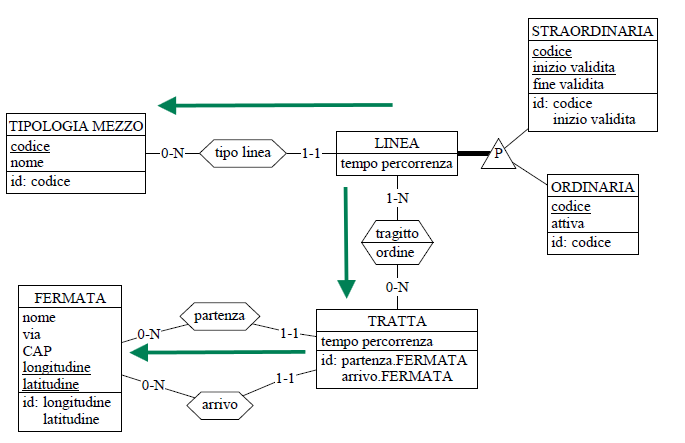
\includegraphics[width=0.7\textwidth]{VisualLineeRid}
    \end{center}
    \begin{table}[H]
    \centering
    \begin{tabular}{|c|c|l|l|}
    \hline
    \textbf{Nome} & \textbf{Tipo} & \textbf{Numero accessi} & \textbf{S/L} \\
    \hline
    LINEA & E & 75 & L \\
    \hline
    TIPOLOGIA MEZZO & E & 75 & L \\
    \hline
    TRAGITTO & A & 1.500 & L \\
    \hline
    TRATTA & E & 150 & L \\
    \hline
    FERMATA (PARTENZA) & E & 75 & L \\
    \hline
    FERMATA (ARRIVO) & E & 75 & L \\
    \hline
    \multicolumn{4}{c}{\textbf{Totale}} \\
    \multicolumn{4}{c}{${A_{lettura}}$ = 1.950, ${A_{scrittura}}$ = 0} \\
    \hline
    \end{tabular}
    \end{table}
    \begin{center}
    ${C_{tot} = {O_{settimana}}\cdot{A_{lettura}}= 7.800.000}$
    \end{center}

    \item \textbf{Analisi senza attributo ridondante \texttt{attiva} su \texttt{ORDINARIA}}
    \begin{center}
    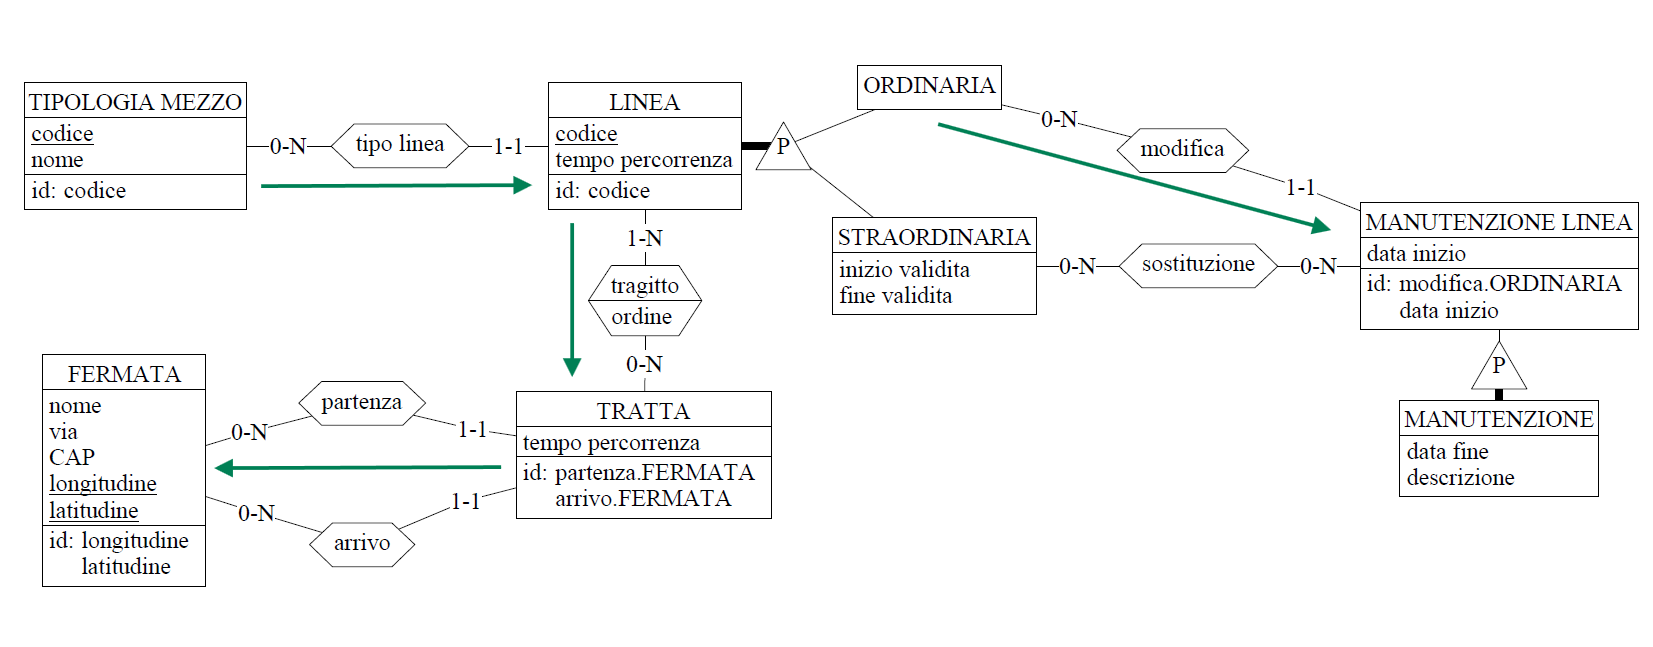
\includegraphics[width=0.9\textwidth]{VisualLineeNoRid}
    \end{center}
    \begin{table}[H]
    \centering
    \begin{tabular}{|c|c|l|l|}
    \hline
    \textbf{Nome} & \textbf{Tipo} & \textbf{Numero accessi} & \textbf{S/L} \\
    \hline
    LINEA & E & 75 & L \\
    \hline
    MANUTENZIONE LINEA & E & 10 & L \\
    \hline
    TIPOLOGIA MEZZO & E & 75 & L \\
    \hline
    TRAGITTO & A & 1.500 & L \\
    \hline
    TRATTA & E & 150 & L \\
    \hline
    FERMATA (PARTENZA) & E & 75 & L \\
    \hline
    FERMATA (ARRIVO) & E & 75 & L \\
    \hline
    \multicolumn{4}{c}{\textbf{Totale}} \\
    \multicolumn{4}{c}{${A_{lettura}}$ = 1.960, ${A_{scrittura}}$ = 0} \\
    \hline
    \end{tabular}
    \end{table}
    \begin{center}
    ${C_{tot} = {O_{settimana}}\cdot{A_{lettura}}= 7.840.000}$
    \end{center}
    \end{itemize}

  % -------------------------------------------------------------------------------------------------------------------------------------------
  % -------------------------------------------------------------------------------------------------------------------------------------------

        \item \textbf{Visualizzazione fermate e orari di una linea} \label{op2} \\
        \[ {O_{settimana} = 3.500} \]
        Dobbiamo visualizzare le linee, i suoi orari e le fermate fatte da essa per qualsiasi utente.
        \begin{center}
	    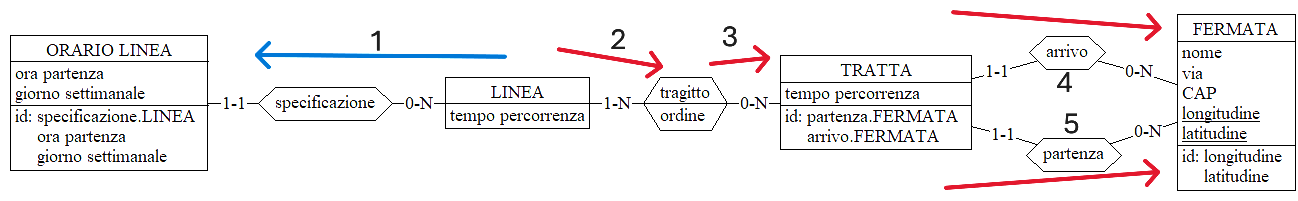
\includegraphics[width=0.9\textwidth]{op_2}
	    \end{center}
        \begin{table}[H]
	\centering
        \begin{tabular}{|c|c|l|l|}
        \hline
        \textbf{Nome} & \textbf{Tipo} & \textbf{Numero accessi} & \textbf{S/L} \\
        \hline
        LINEA & E & 1 & L \\
        \hline
        ORARIO LINEA & E & 20 & L \\
        \hline
        TRAGITTO & A & 20 & L \\
        \hline
        TRATTA & E & 20 & L \\
        \hline
        FERMATA & E & 40 & L \\
        \hline
        \multicolumn{4}{c}{\textbf{Totale}} \\
        \multicolumn{4}{c}{${A_{lettura}}$ = 71, ${A_{scrittura}}$ = 0} \\
        \hline
        \end{tabular}
        \end{table}
        \begin{center}
        ${C_{tot} = {O_{settimana}}\cdot{A_{lettura}} = 248.500}$
        \end{center}

  % -------------------------------------------------------------------------------------------------------------------------------------------
  % -------------------------------------------------------------------------------------------------------------------------------------------

        \item \textbf{Visualizzazione degli hub mobilità} \label{op3} \\
	\[{O_{settimana} = 500}\]
	Questa operazione deve poter essere fatta da qualsiasi persona che accede all'applicativo. Si richiede per ogni \texttt{HUB MOBILITA} di visualizzare:
	\begin{itemize}
	\renewcommand\labelitemi{--}
	    \item Tutti gli attributi di \texttt{HUB MOBILITA}
	    \item I tipi di \texttt{CONTENUTO HUB} per ogni \texttt{HUB MOBILITA}
	    \item I posti rimanenti per ogni \texttt{CONTENUTO HUB} nell'\texttt{HUB MOBILITA}
	    \item L'eventuale fermata a cui è collegato
	\end{itemize}
	\begin{center}
	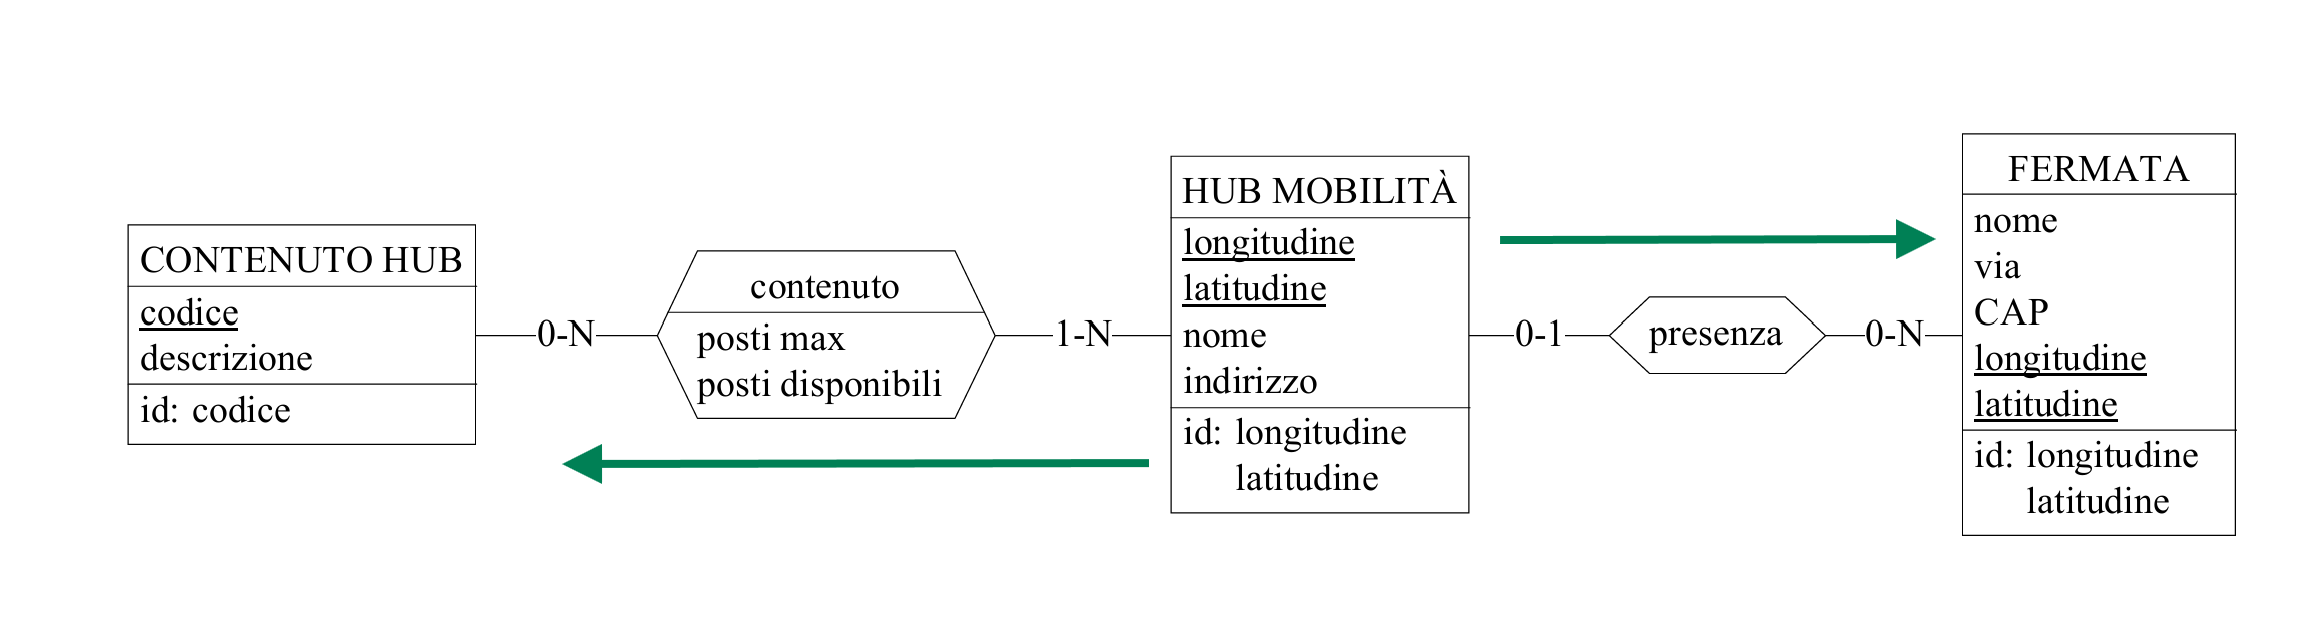
\includegraphics[width=0.9\textwidth]{VisualHubMobilita}
	\end{center}
    \begin{table}[H]
    \centering
	\begin{tabular}{|l|c|c|c|}
	\hline
	Nome & Tipo & Numero Accessi & S/L \\
	\hline
	HUB MOBILITA & E & 225 & L \\
	\hline
	CONTENUTO & A & 225 $\times$ 2 & L \\
	\hline
	CONTENUTO HUB & E & 225 $\times$ 2 & L \\
	\hline
	FERMATA & E & 165 & L \\
	\hline
        \multicolumn{4}{c}{\textbf{Totale}} \\
        \multicolumn{4}{c}{${A_{lettura}}$ = 1290, ${A_{scrittura}}$ = 0} \\
        \hline
	\end{tabular}
    \end{table}
    \begin{center}
    ${C_{tot} = {O_{settimana}}\cdot{A_{lettura}}= 645.000}$
    \end{center}

  % -------------------------------------------------------------------------------------------------------------------------------------------
  % -------------------------------------------------------------------------------------------------------------------------------------------

         \item \textbf{Visualizzazione orario e linee assegnate agli autisti} \label{op4} \\
            \[ {O_{settimana} = 150} \]
           \begin{itemize}
            \item \textbf{Analisi con attributo ridondante \texttt{tempo percorrenza} su \texttt{LINEA}} \\
            Dobbiamo visualizzare l'orario di lavoro di un autista, mostrando la linea l'orario e il mezzo assegnato.
            La lettura partirà da un autista; il numero di letture è stato calcolato dividendo il numero totale delle entità attuazione corsa (250.000) con il numero totale degli autisti (130), in modo da trovare la media di associazioni per ogni autista.
            \begin{center}
	        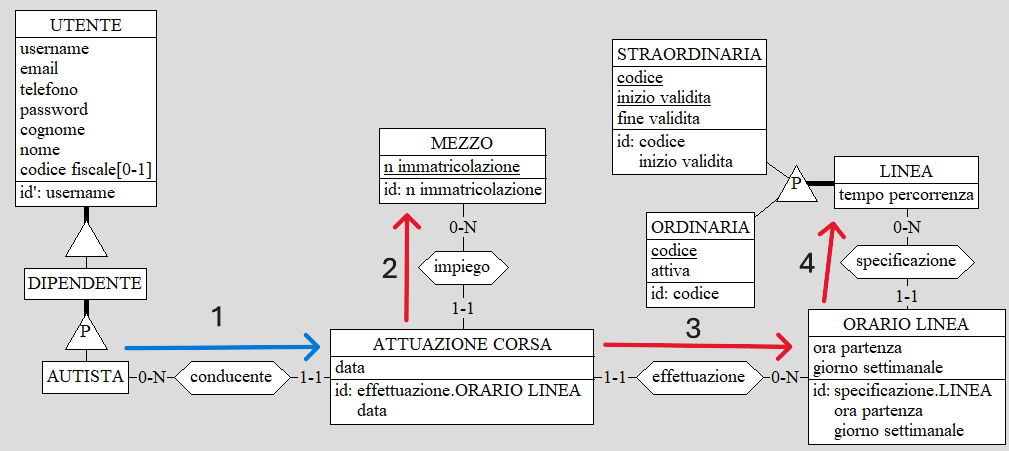
\includegraphics[width=0.9\textwidth]{op_4_RID}
	        \end{center}
            \begin{table}[H]
            \centering
            \begin{tabular}{|c|c|l|l|}
            \hline
            \textbf{Nome} & \textbf{Tipo} & \textbf{Numero accessi} & \textbf{S/L} \\
            \hline
            AUTISTA & E & 1 & L \\
            \hline
            ATTUAZIONE CORSA & E & 1923 & L \\
            \hline
            ORARIO LINEA & E & 1923 & L \\
            \hline
            LINEA & E & 1923 & L \\
            \hline
            MEZZO & E & 1923 & L \\
            \hline
            \multicolumn{4}{c}{\textbf{Totale}} \\
            \multicolumn{4}{c}{${A_{lettura}}$ = 7693, ${A_{scrittura}}$ = 0} \\
            \hline
            \end{tabular}
            \end{table}
            \begin{center}
            ${C_{tot} = {O_{settimana}}\cdot {A_{lettura}} =1.153.950}$
            \end{center}

            \item \textbf{Analisi senza attributo ridondante \texttt{tempo percorrenza} su \texttt{LINEA}} \\
            Dobbiamo visualizzare l'orario di lavoro di un autista, mostrando la linea l'orario e il mezzo assegnato.
            La lettura partirà da un autista, le letture sono state calcolate nello stesso modo.\\
            Visto che non abbiamo il tempo di percorrenza su \texttt{LINEA}, dobbiamo ricavarlo tramite le varie \texttt{TRATTE} che compongono la linea. Ogni \texttt{LINEA} ha in media 20 associazioni \texttt{TRAGITTO}.
            \begin{center}
	        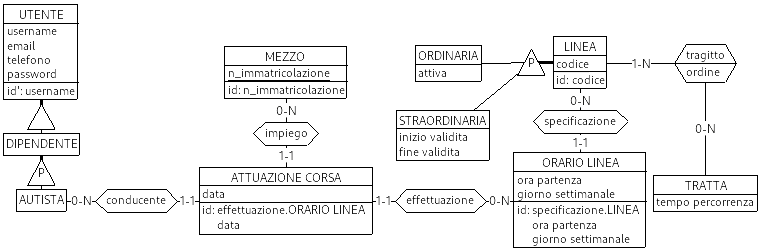
\includegraphics[width=0.9\textwidth]{op_4_NORID}
	        \end{center}
            \begin{table}[H]
            \centering
            \begin{tabular}{|c|c|l|l|}
            \hline
            \textbf{Nome} & \textbf{Tipo} & \textbf{Numero accessi} & \textbf{S/L} \\
            \hline
            AUTISTA & E & 1 & L \\
            \hline
            ATTUAZIONE CORSA & E & 1.923 & L \\
            \hline
            ORARIO LINEA & E & 1.923 & L \\
            \hline
            MEZZO & E & 1.923 & L \\
            \hline
            LINEA & E & 1.923 & L \\
            \hline
            TRAGITTO & A & 38.460 & L \\
            \hline
            TRATTA & E & 38.460 & L \\
            \hline
            \multicolumn{4}{c}{\textbf{Totale}} \\
            \multicolumn{4}{c}{${A_{lettura}}$ = 84.613, ${A_{scrittura}}$ = 0} \\
            \hline
            \end{tabular}
            \end{table}
            \begin{center}
            ${C_{tot} = {O_{settimana}}\cdot {A_{lettura}} =12.691.950}$
            \end{center}
    \end{itemize}


  % -------------------------------------------------------------------------------------------------------------------------------------------
  % -------------------------------------------------------------------------------------------------------------------------------------------

    \item \textbf{Visualizzazione orario e linee assegnate ai controllori} \label{op5} \\
    \[ {O_{settimana} = 100} \]
    Questa operazione serve a un controllore per visualizzare il suo orario di lavoro e come dovrà essere svolto (ovvero le linee che dovrà controllare). Poiché è necessario calcolare l'orario di arrivo della linea, l'attributo \texttt{tempo percorrenza} su \texttt{LINEA} rende superfluo il calcolo del tempo tramite la somma dei tempi di tutte le \texttt{TRATTA}: è quindi necessario eseguire i calcoli dei costi con attributo ridondante e non. \\
    Nei conti terremo conto del fatto che l'operazione è relativa a un solo giorno, ovvero sarà eseguito un filtro delle \texttt{ATTUAZIONE CORSA}. \\
    Dati un controllore e una data, bisogna quindi visualizzare:
    \begin{itemize}
    \renewcommand\labelitemi{--}
    \item L'orario di partenza, di arrivo e il codice della \texttt{LINEA} da controllare
    \item Il numero di immatricolazione del \texttt{MEZZO} che effettua la corsa
    \end{itemize}

    \begin{itemize}
    \item \textbf{Analisi con attributo ridondante \texttt{tempo percorrenza} su \texttt{LINEA}}
    \begin{center}
    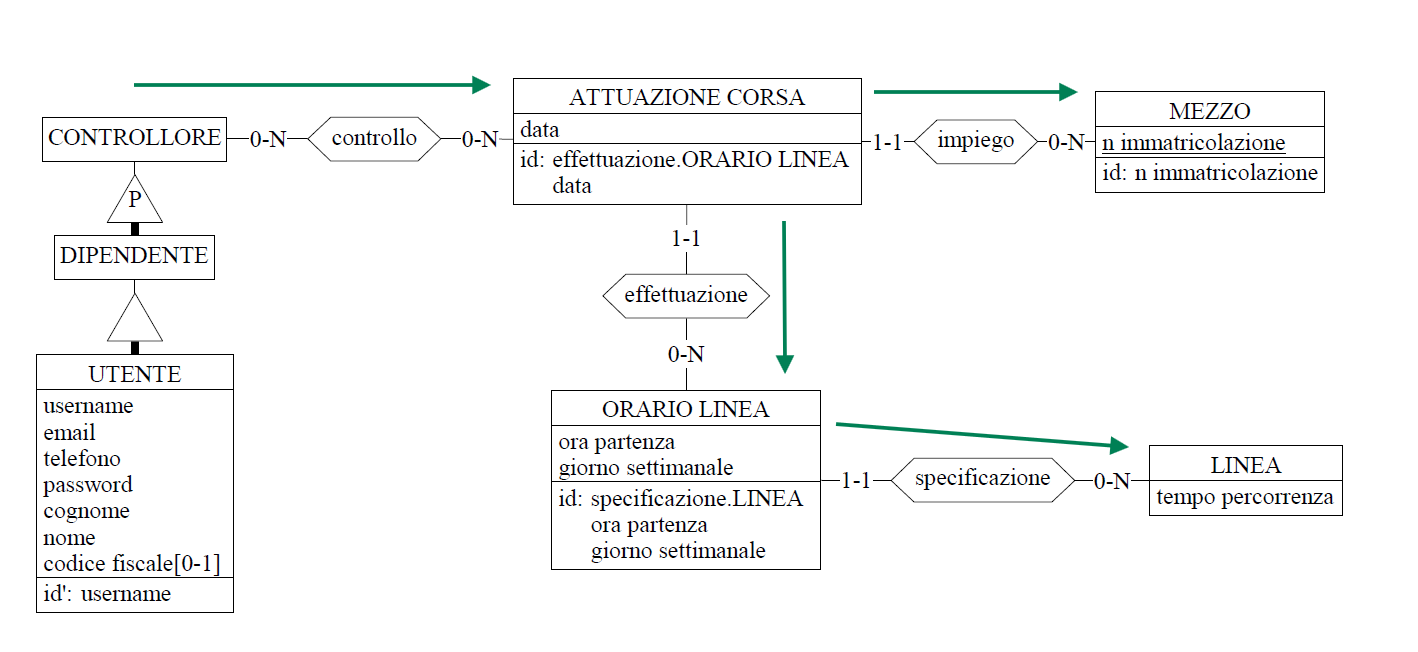
\includegraphics[width=0.9\textwidth]{VisualOrarioControlloriRid}
    \end{center}
    \begin{table}[H]
    \centering
    \begin{tabular}{|c|c|l|l|}
    \hline
    \textbf{Nome} & \textbf{Tipo} & \textbf{Numero accessi} & \textbf{S/L} \\
    \hline
    CONTROLLORE & E & 1 & L \\
    \hline
    CONTROLLO & A & 1.250 & L \\
    \hline
    ATTUAZIONE CORSA & E & 1.250 & L \\
    \hline
    ORARIO LINEA & E & 7 & L \\
    \hline
    LINEA & E & 7 & L \\
    \hline
    MEZZO & E & 7 & L \\
   \hline
    \multicolumn{4}{c}{\textbf{Totale}} \\
    \multicolumn{4}{c}{${A_{lettura}}$ = 2.522, ${A_{scrittura}}$ = 0} \\
    \hline
    \end{tabular}
    \end{table}
    \begin{center}
    ${C_{tot} = {O_{settimana}}\cdot{A_{lettura}}= 252.200}$
    \end{center}

    \item \textbf{Analisi senza attributo ridondante \texttt{tempo percorrenza} su \texttt{LINEA}}
    \begin{center}
    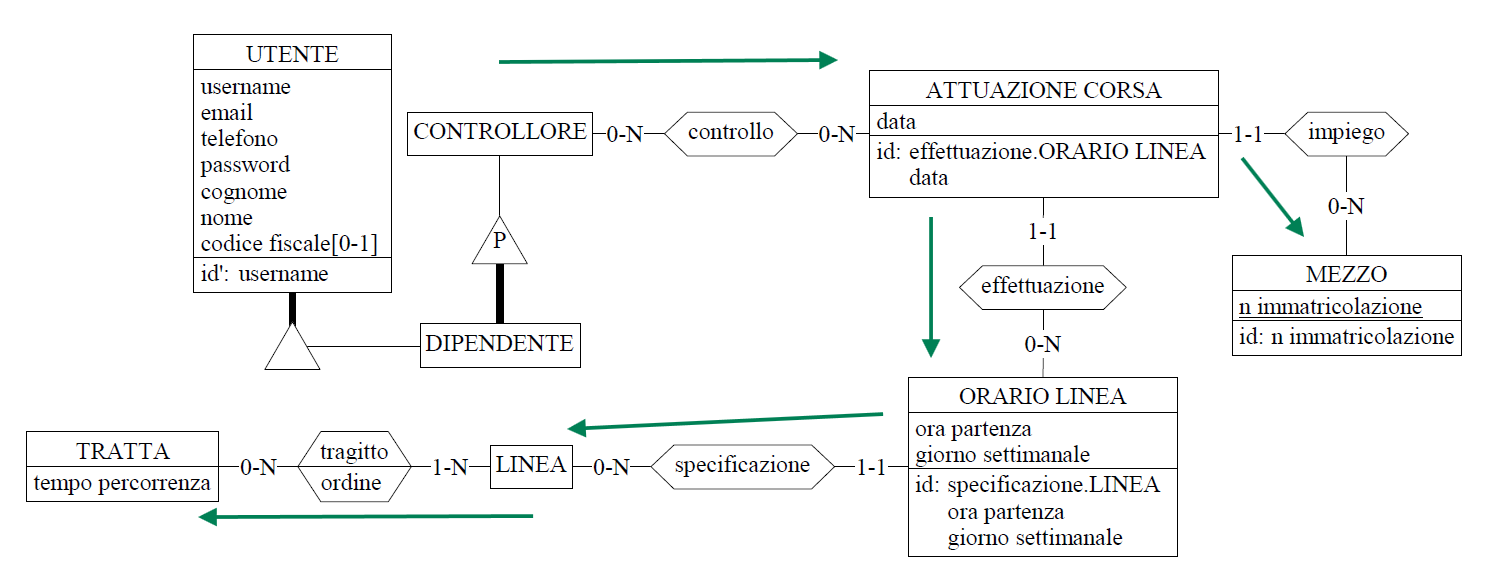
\includegraphics[width=0.9\textwidth]{VisualOrarioControlloriNoRid}
    \end{center}
    \begin{table}[H]
    \centering
    \begin{tabular}{|c|c|l|l|}
    \hline
    \textbf{Nome} & \textbf{Tipo} & \textbf{Numero accessi} & \textbf{S/L} \\
    \hline
    CONTROLLORE & E & 1 & L \\
    \hline
    CONTROLLO & A & 1.250 & L \\
    \hline
    ATTUAZIONE CORSA & E & 1.250 & L \\
    \hline
    ORARIO LINEA & E & 7 & L \\
    \hline
    LINEA & E & 7 & L \\
    \hline
    TRAGITTO & A & 140 & L \\
    \hline
    TRATTA & E & 140 & L \\
    \hline
    MEZZO & E & 7 & L \\
   \hline
    \multicolumn{4}{c}{\textbf{Totale}} \\
    \multicolumn{4}{c}{${A_{lettura}}$ = 2.802, ${A_{scrittura}}$ = 0} \\
    \hline
    \end{tabular}
    \end{table}
    \begin{center}
    ${C_{tot} = {O_{settimana}}\cdot{A_{lettura}}= 280.200}$
    \end{center}
    \end{itemize}

  % -------------------------------------------------------------------------------------------------------------------------------------------
  % -------------------------------------------------------------------------------------------------------------------------------------------

    \item \textbf{Estrazione delle linee con più convalide nell'ultimo mese} \label{op6} \\
    \[ {O_{settimana} = 3} \]
    Dobbiamo estrarre le linee con più biglietti convalidati nell'ultimo mese. Il conteggio per la quantità di letture su \texttt{CONVALIDA} è stato fatto con una media tramite la tabella dei volumi.
    \begin{center}
	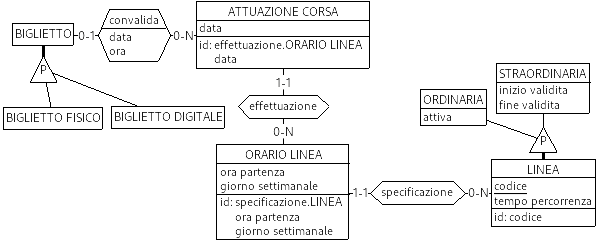
\includegraphics[width=0.9\textwidth]{op_6}
	\end{center}
    \begin{table}[H]
    \centering
    \begin{tabular}{|c|c|l|l|}
    \hline
    \textbf{Nome} & \textbf{Tipo} & \textbf{Numero accessi} & \textbf{S/L} \\
    \hline
    ATTUAZIONE CORSA & E & 250.000 & L \\
    \hline
    CONVALIDA & E & 33.333 & L \\
    \hline
    ORARIO LINEA & E & 1 & L \\
    \hline
    LINEA & E & 1 & L \\
    \hline
    \multicolumn{4}{c}{\textbf{Totale}} \\
    \multicolumn{4}{c}{${A_{lettura}}$ = 283.335, ${A_{scrittura}}$ = 0} \\
    \hline
    \end{tabular}
    \end{table}
    \begin{center}
    ${C_{tot} = {O_{settimana}}\cdot {A_{lettura}} = 850.005}$
    \end{center}

  % -------------------------------------------------------------------------------------------------------------------------------------------
  % -------------------------------------------------------------------------------------------------------------------------------------------

    \item \textbf{Estrazione delle manuntenzioni che coinvolgono un determinato mezzo} \label{op7} \\
    \[ {O_{settimana} = 5} \]
    Questa operazione serve per visualizzare tutte le manutenzioni che sono state effettuate ad un mezzo.\\
    Dato un mezzo bisogna quindi visualizzare:
    \begin{itemize}
    \renewcommand\labelitemi{--}
    \item Tutti i dati della \texttt{MANUTENZIONE}
    \item La partita iva dell'eventuale \texttt{AZIENDA} esterna incaricata della manutenzione
    \end{itemize}
    \begin{center}
    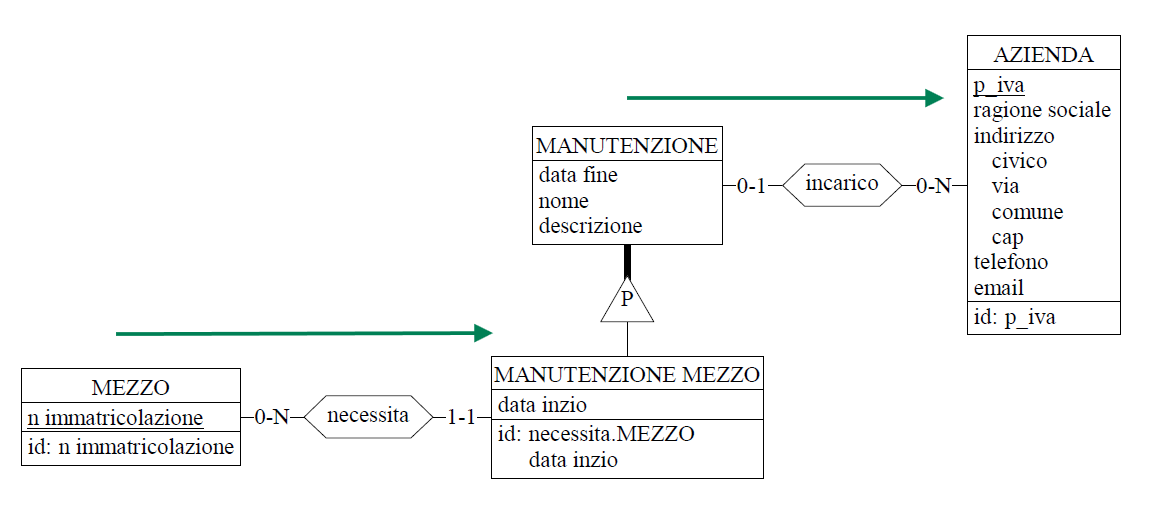
\includegraphics[width=0.8\textwidth]{VisualManutenzioniMezzo}
    \end{center}
    \begin{table}[H]
    \centering
    \begin{tabular}{|c|c|l|l|}
    \hline
    \textbf{Nome} & \textbf{Tipo} & \textbf{Numero accessi} & \textbf{S/L} \\
    \hline
    MEZZO & E & 1 & L \\
    \hline
    MANUTENZIONE MEZZO & E & 4 & L \\
    \hline
    AZIENDA & E & 2 & L \\
    \hline
    \multicolumn{4}{c}{\textbf{Totale}} \\
    \multicolumn{4}{c}{${A_{lettura}}$ = 7, ${A_{scrittura}}$ = 0} \\
    \hline
    \end{tabular}
    \end{table}
    \begin{center}
    ${C_{tot} = {O_{settimana}}\cdot{A_{lettura}}= 35}$
    \end{center}

  % -------------------------------------------------------------------------------------------------------------------------------------------
  % -------------------------------------------------------------------------------------------------------------------------------------------

    \item \textbf{Estrazione delle manuntenzioni ed eventuali linee sostitutive che coinvolgono una linea (Variazioni di servizio)} \label{op8} \\
	\[{O_{settimana} = 5}\]
	Questa operazione deve poter essere effettuata da qualsiasi utente. Consente di visualizzare le variazioni di servizio di una specifica linea.\\
	Specificata una linea, va estratto:
	\begin{itemize}
	\renewcommand\labelitemi{--}
	    \item Tutti gli attributi di \texttt{MANUNTENZIONE LINEA} e \texttt{MANUNTENZIONE}
	    \item L'azienda che effettua la manuntezione
	    \item Tutte le linee straordinarie (codice, inizioValidita, fineValidita, partenza, arrivo) con cui viene sostituita la linea
	\end{itemize}

	\begin{center}
	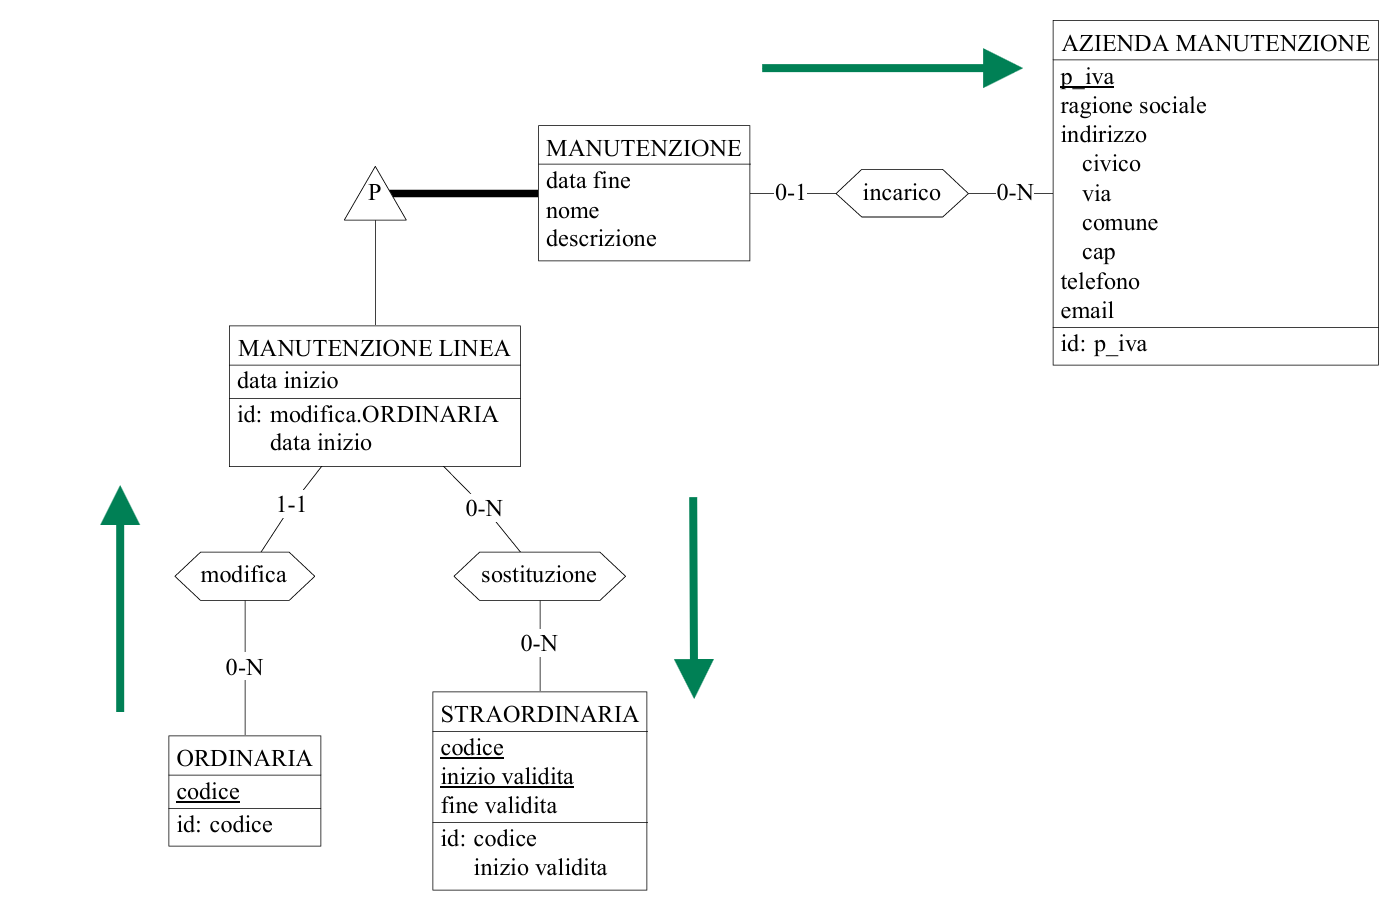
\includegraphics[width=0.8\textwidth]{VisualManunLinee}
	\end{center}
	\begin{table}[H]
	\centering
	\begin{tabular}{|l|c|c|c|}
	\hline
	Nome & Tipo & Numero Accessi & S/L \\
	\hline
	ORDINARIA & E & 1 & L \\
	\hline
	MANUNTENZIONE LINEA & E & 10 & L \\
	\hline
	AZIENDA & E & 10 & L \\
	\hline
	SOSTITUZIONE & A & 1 $\times$ 10 & L \\
	\hline
	STRAORDINARIA & E & 1 $\times$ 10 & L \\
          \hline
          \multicolumn{4}{c}{\textbf{Totale}} \\
          \multicolumn{4}{c}{${A_{lettura}}$ = 41, ${A_{scrittura}}$ = 0} \\
          \hline
	\end{tabular}
	\end{table}
	    \begin{center}
	    ${C_{tot} = {O_{settimana}}\cdot{A_{lettura}}= 205}$
	    \end{center}

  % -------------------------------------------------------------------------------------------------------------------------------------------
  % -------------------------------------------------------------------------------------------------------------------------------------------

	\item \textbf{Visualizzazione incassi dati dalle convalide per una linea} \label{op9} \\
    \[ {O_{settimana} = 10} \]
    Partendo da una linea dobbiamo visualizzare gli incassi fatti da essa tramite i biglietti convalidati.
    \begin{center}
	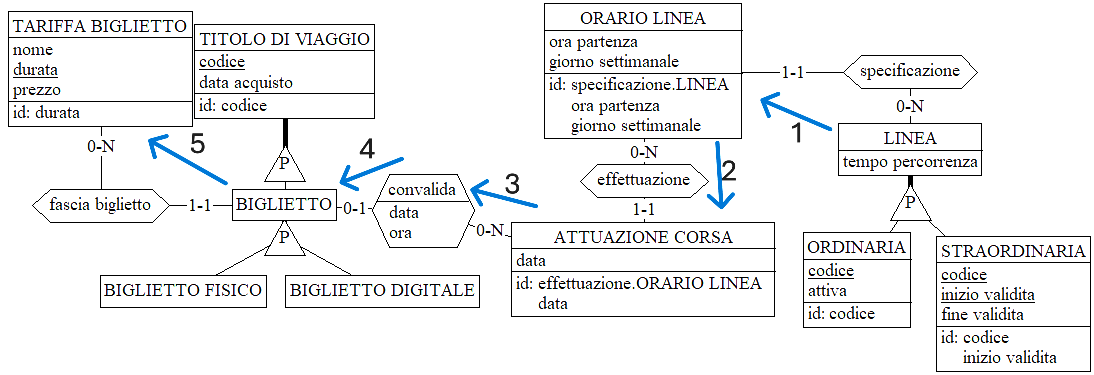
\includegraphics[width=0.9\textwidth]{op_9}
	\end{center}
    \begin{table}[H]
    \centering
    \begin{tabular}{|c|c|l|l|}
    \hline
    \textbf{Nome} & \textbf{Tipo} & \textbf{Numero accessi} & \textbf{S/L} \\
    \hline
    LINEA & E & 1 & L \\
    \hline
    ORARIO LINEA & E & 20 & L \\
    \hline
    ATTUAZIONE CORSA & E & 167 & L \\
    \hline
    CONVALIDA & A & 209 & L \\
    \hline
    BIGLIETTO & E & 209 & L \\
    \hline
    TARIFFA BIGLIETTO & E & 209 & L \\
    \hline
    \multicolumn{4}{c}{\textbf{Totale}} \\
    \multicolumn{4}{c}{${A_{lettura}}$ = 815, ${A_{scrittura}}$ = 0} \\
    \hline
    \end{tabular}
    \end{table}
    \begin{center}
    ${C_{tot} = {O_{settimana}}\cdot {A_{lettura}} = 8.150}$
    \end{center}

  % -------------------------------------------------------------------------------------------------------------------------------------------
  % -------------------------------------------------------------------------------------------------------------------------------------------


    \item\textbf{Estrazione degli incassi per tipo di tariffa dei biglietti in periodo definito} \label{op10} \\
    \[ {O_{settimana} = 5} \]
    Vogliamo visualizzare gli incassi di una specifica tariffa dei biglietti in un certo periodo di tempo; per eseguire i calcoli considereremo come periodo una settimana. Per rendere la stima più realistica non terremo conto della data di acquisto dei biglietti, ma della data dell'effettiva convalida.
    Data una certa tariffa dei biglietti e l'intervallo di tempo vogliamo quindi visualizzare:
    \begin{itemize}
	\renewcommand\labelitemi{--}
    \item Il numero di \texttt{CONVALIDA} nel dato periodo di tempo
    \item L'incasso totale, ovvero il prezzo della \texttt{TARIFFA BIGLIETTO} data per il numero di convalide
    \end{itemize}
    \begin{center}
    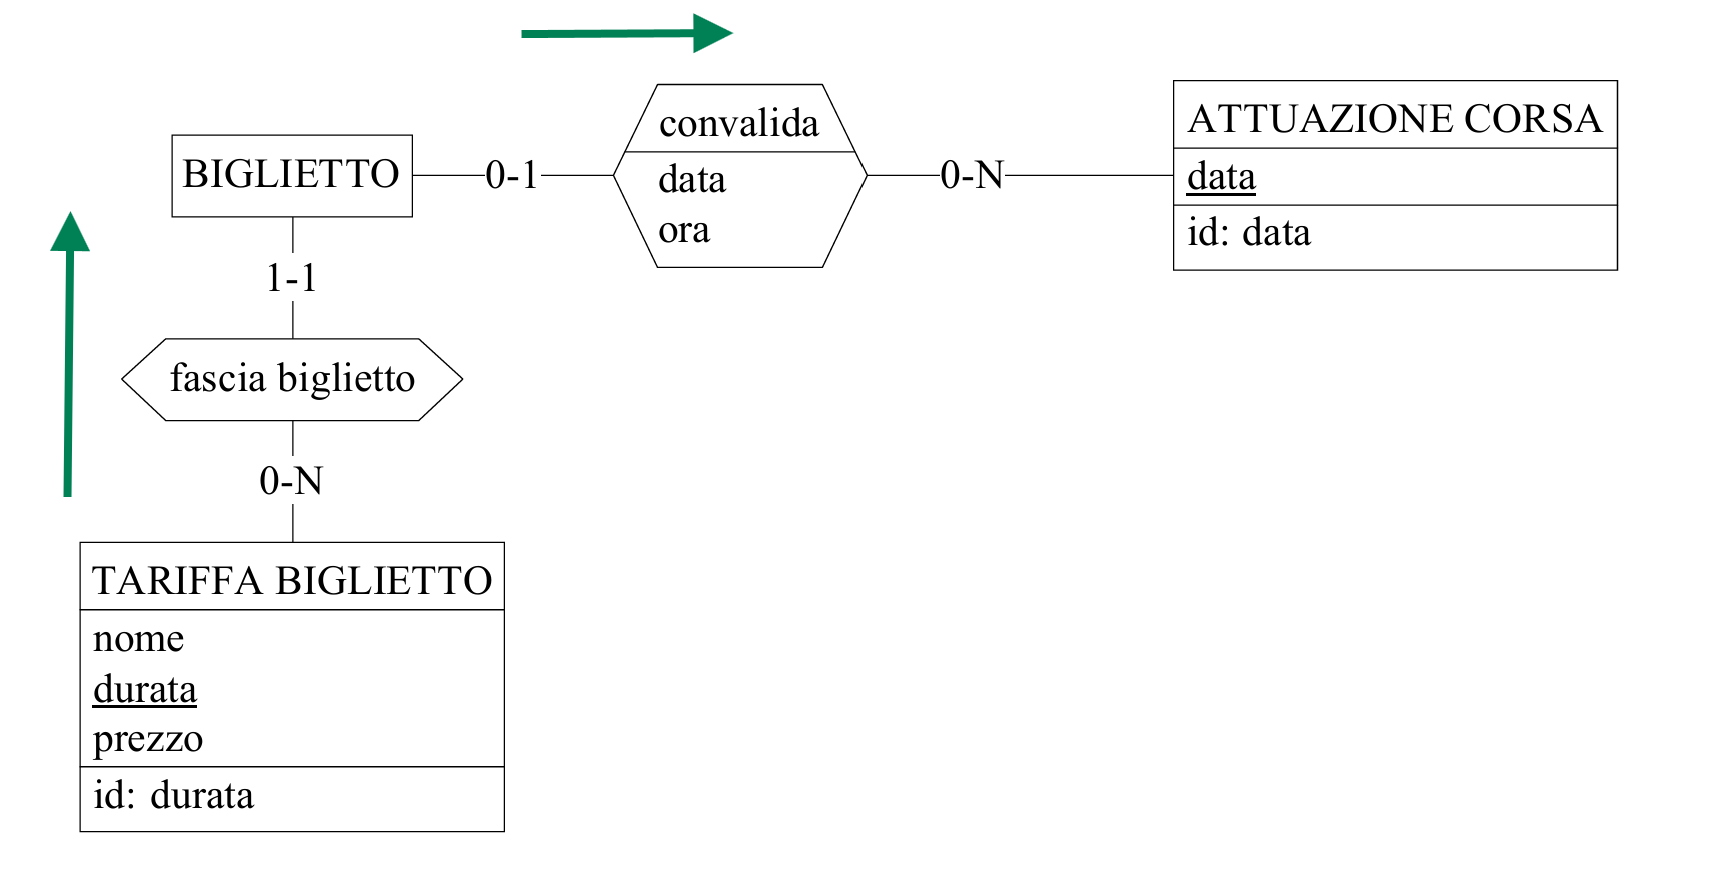
\includegraphics[width=0.7\textwidth]{VisualIncassoPerTariffa}
    \end{center}
    \begin{table}[H]
    \centering
    \begin{tabular}{|c|c|l|l|}
    \hline
    \textbf{Nome} & \textbf{Tipo} & \textbf{Numero accessi} & \textbf{S/L} \\
    \hline
    TARIFFA BIGLIETTO & E & 1 & L \\
    \hline
    BIGLIETTO & E & 30.000 & L \\
    \hline
    CONVALIDA & A & 20.000 & L \\
    \hline
    \multicolumn{4}{c}{\textbf{Totale}} \\
    \multicolumn{4}{c}{${A_{lettura}}$ = 50.001, ${A_{scrittura}}$ = 0} \\
    \hline
    \end{tabular}
    \end{table}
    \begin{center}
    ${C_{tot} = {O_{settimana}}\cdot{A_{lettura}}= 250.005}$
    \end{center}

  % -------------------------------------------------------------------------------------------------------------------------------------------
  % -------------------------------------------------------------------------------------------------------------------------------------------

    \item\textbf{Estrazione delle linee con più multe in periodo definito} \label{op11} \\
	\[{O_{settimana} = 2}\]
	Questa operazione deve poter essere effettuata dall'amministratore di sistema.\\
	Per ogni linea va estratto:
	\begin{itemize}
	\renewcommand\labelitemi{--}
	    \item Il codice della linea
	    \item Il numero di multe ottenute negli in un periodo definito
	\end{itemize}
	\begin{center}
	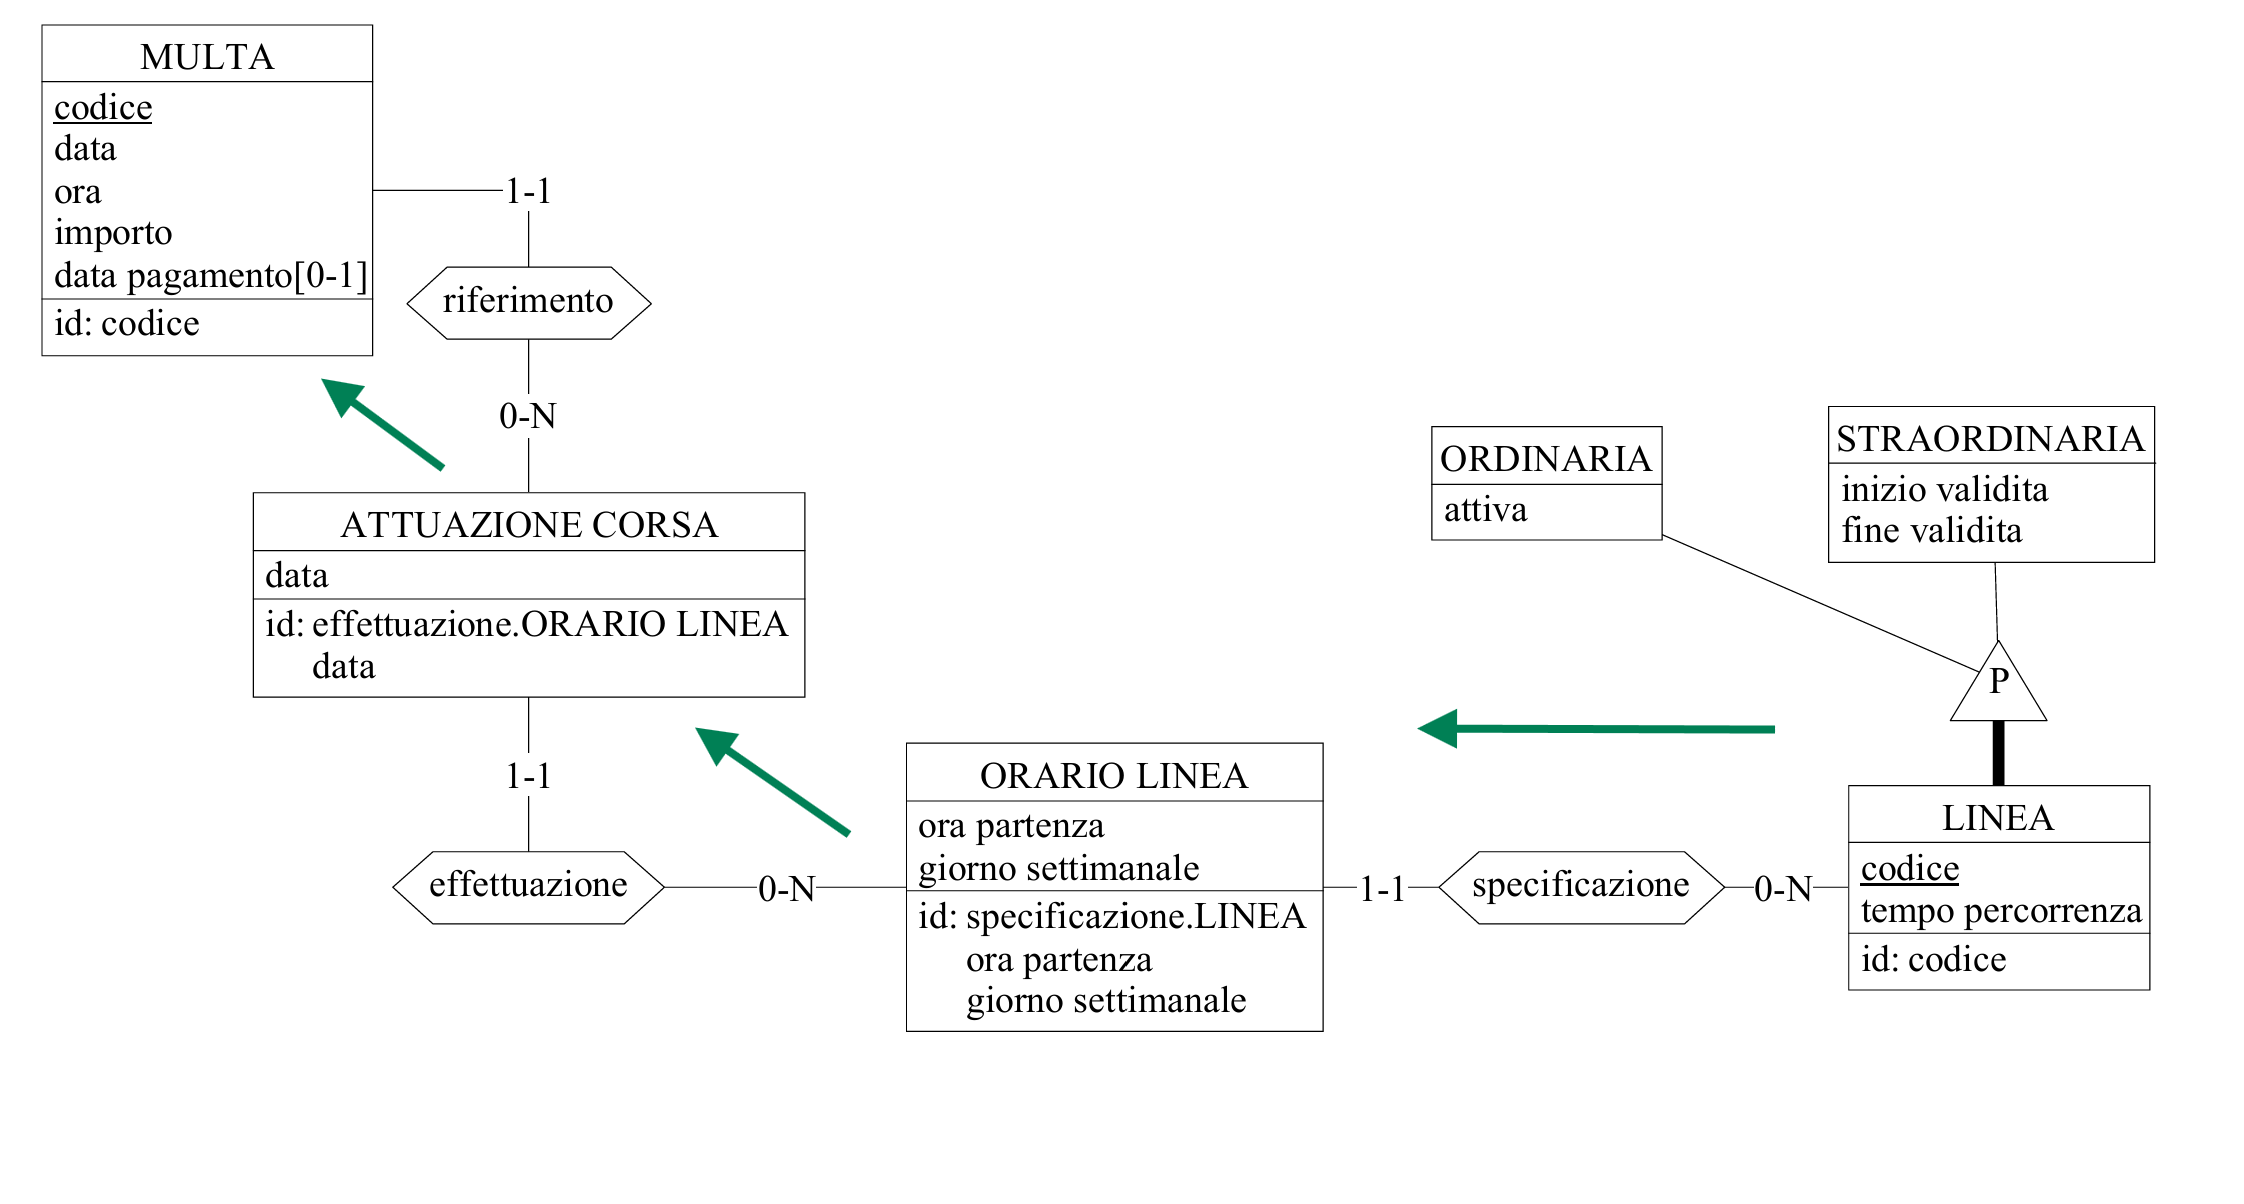
\includegraphics[width=0.7\textwidth]{VisualLineeConPiuMulte}
	\end{center}

	\begin{table}[H]
	\centering
	\begin{tabular}{|l|c|c|c|}
	\hline
	Nome & Tipo & Numero Accessi & S/L \\
	\hline
	LINEA & E & 75 & L \\
	\hline
	ORARIO LINEA & E & 75 $\times$ 20 & L \\
	\hline
	ATTUAZIONE CORSA & E & 3333 $\times$ 75 & L \\
	\hline
	MULTA & E & 0.04 $\times$ 75 & L \\
	    \hline
	    \multicolumn{4}{c}{\textbf{Totale}} \\
	    \multicolumn{4}{c}{${A_{lettura}}$ = 251.850, ${A_{scrittura}}$ = 0} \\
	    \hline
	\end{tabular}
	\end{table}
	    \begin{center}
	    ${C_{tot} = {O_{settimana}}\cdot{A_{lettura}}= 503.700}$
	    \end{center}


  % -------------------------------------------------------------------------------------------------------------------------------------------
  % -------------------------------------------------------------------------------------------------------------------------------------------

	\item \textbf{Estrazione delle 5 linee con manutenzioni più gravose (in termini di linee sostitutive e durata)} \label{op12} \\
	    \[ {O_{settimana} = 2} \]
	    Dobbiamo visualizzare le linee con le manutenzioni più gravose, a livello applicativo verrà calcolato un "punteggio" che indicherà quanto sia gravosa una manutenzione:
	    \begin{itemize}
		\renewcommand\labelitemi{--}
	        \item +5 pti ogni linea straordinaria dovuta alla manutenzione
	        \item +1 pto ogni 3 giorni di lavoro sulla  linea.
	    \end{itemize}
        \begin{center}
	    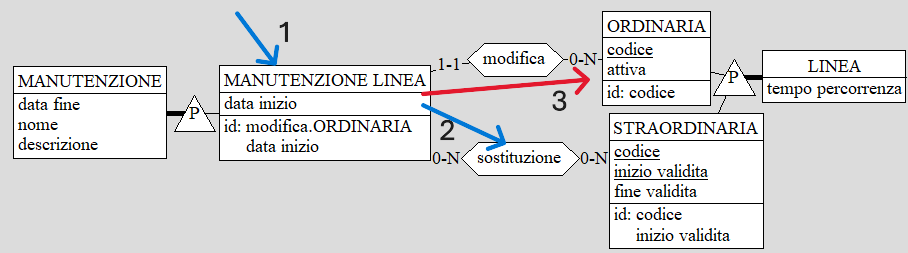
\includegraphics[width=0.9\textwidth]{op_12}
	    \end{center}
	    \begin{table}[H]
	    \centering
	    \begin{tabular}{|c|c|l|l|}
	    \hline
	    \textbf{Nome} & \textbf{Tipo} & \textbf{Numero accessi} & \textbf{S/L} \\
	    \hline
	    MANUTENZIONE LINEA & E & 10 & L \\
	    \hline
	    SOSTITUZIONE & A & 10 & L \\
	    \hline
	    LINEA ORDINARIA & E & 5 & L \\
	    \hline
	    \multicolumn{4}{c}{\textbf{Totale}} \\
	    \multicolumn{4}{c}{${A_{lettura}}$ = 25, ${A_{scrittura}}$ = 0} \\
	    \hline
	    \end{tabular}
	    \end{table}
	    \begin{center}
	    ${C_{tot} = {O_{settimana}}\cdot {A_{lettura}} = 100}$
	    \end{center}

  % -------------------------------------------------------------------------------------------------------------------------------------------
  % -------------------------------------------------------------------------------------------------------------------------------------------
	\item \textbf{Estrazione delle linee con $>5$ controlli/giorno e $\leq 10$ multe/giorno} \label{op13} \\
	\[{O_{settimana} = 3}\]
	Questa operazione deve poter essere effettuata dall'amministratore di sistema.\\
	Devono essere estratti i codici delle linee che rispettano la seguente condizione:
	\[
	\text{controllo} > 5/\text{giorno} \cap \text{multe} \leq 10/\text{giorno}
	\]

	\begin{center}
	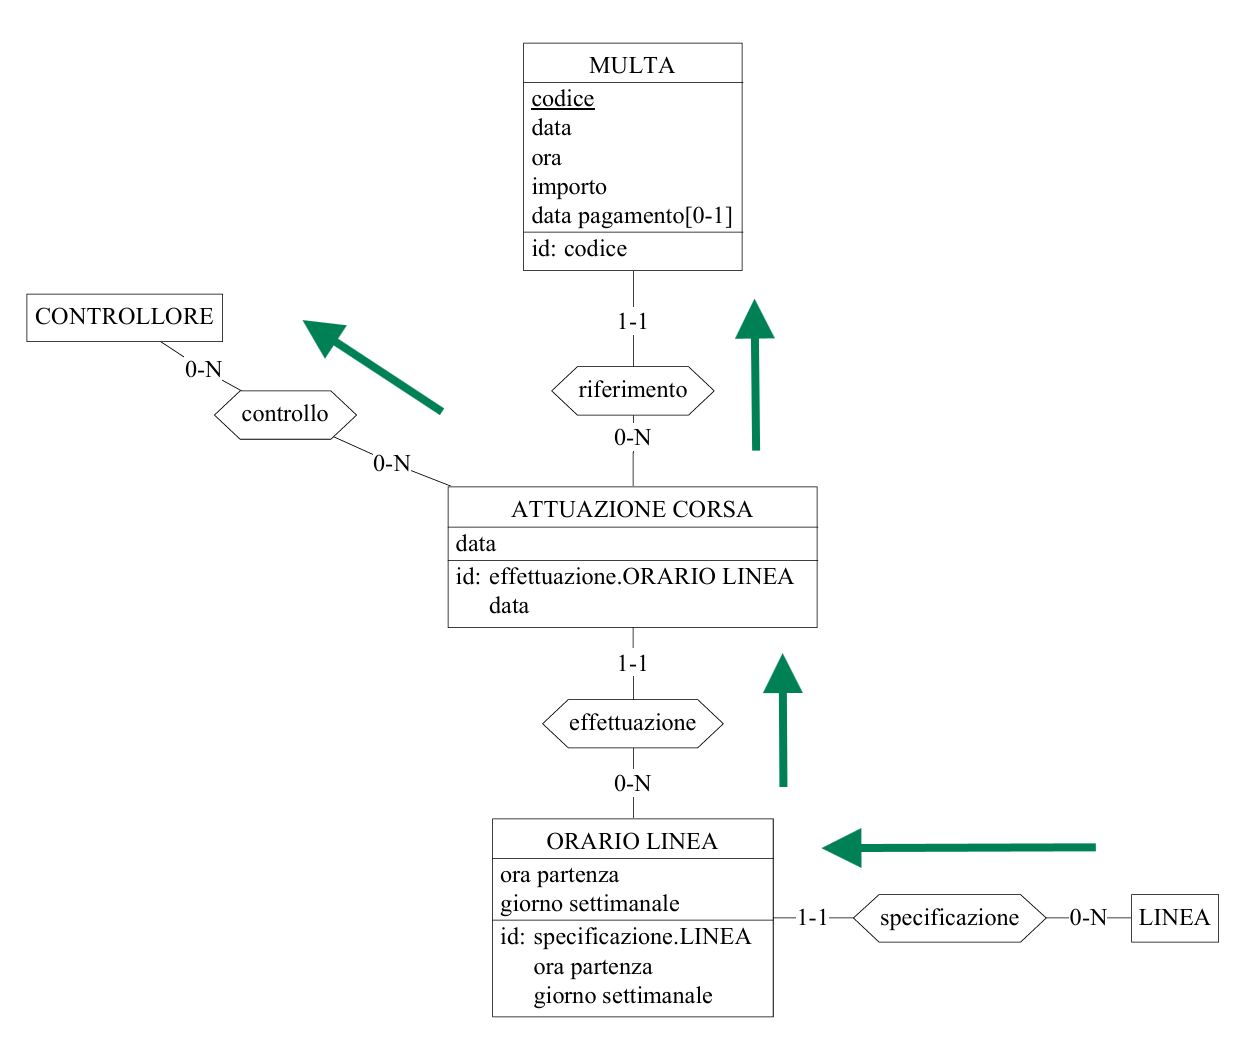
\includegraphics[width=0.7\textwidth]{VisualLineeMulteControlli}
	\end{center}

	\begin{table}[H]
	\centering
	\begin{tabular}{|l|c|c|c|}
	\hline
	Nome & Tipo & Numero Accessi & S/L \\
	\hline
	LINEA & E & 75 & L \\
	\hline
	ORARIO LINEA & E & 20 $\times$ 75 & L \\
	\hline
	ATTUAZIONE CORSA & E & 3333 $\times$ 75 & L \\
	\hline
	CONTROLLO & A & 0.2 $\times$ 75 & L \\
	    \hline
	    \multicolumn{4}{c}{\textbf{Totale}} \\
	    \multicolumn{4}{c}{${A_{lettura}}$ = 251.700, ${A_{scrittura}}$ = 0} \\
	    \hline
	\end{tabular}
	\end{table}
	    \begin{center}
	    ${C_{tot} = {O_{settimana}}\cdot {A_{lettura}} = 755.100}$
	    \end{center}

  % -------------------------------------------------------------------------------------------------------------------------------------------
  % -------------------------------------------------------------------------------------------------------------------------------------------

    \item \textbf{Visualizzazione delle linee con il maggior tempo di percorrenza} \label{op14} \\
            \[ {O_{settimana} = 2} \]
           \begin{itemize}
            \item \textbf{Analisi con attributo ridondante \texttt{tempo percorrenza} su \texttt{LINEA}} \\
        In questo caso basterà leggere il dato del tempo di percorrenza dalla relativa linea.
        \begin{table}[H]
        \centering
        \begin{tabular}{|c|c|l|l|}
        \hline
        \textbf{Nome} & \textbf{Tipo} & \textbf{Numero accessi} & \textbf{S/L} \\
        \hline
        LINEA & E & 75 & L \\
        \hline
        \multicolumn{4}{c}{\textbf{Totale}} \\
        \multicolumn{4}{c}{${A_{lettura}}$ = 75, ${A_{scrittura}}$ = 0} \\
        \hline
        \end{tabular}
        \end{table}
        \begin{center}
        ${C_{tot} = {O_{settimana}}\cdot {A_{lettura}} = 150}$
        \end{center}

            \item \textbf{Analisi senza attributo ridondante \texttt{tempo percorrenza} su \texttt{LINEA}} \\
        In questo caso invece dovremmo calcolare il tempo di percorrenza leggendo tutte le \texttt{tratte} di cui è composta la relativa linea.
        \begin{center}
	    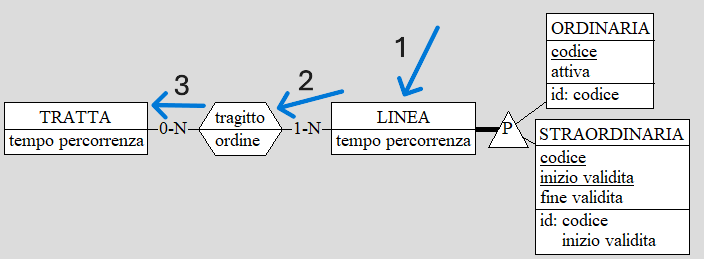
\includegraphics[width=0.7\textwidth]{op_14_NORID}
	    \end{center}
        \begin{table}[H]
        \centering
        \begin{tabular}{|c|c|l|l|}
        \hline
        \textbf{Nome} & \textbf{Tipo} & \textbf{Numero accessi} & \textbf{S/L} \\
        \hline
        LINEA & E & 75 & L \\
        \hline
        TRAGITTO & A & 1.500 & L \\
        \hline
        TRATTA & E & 1.500 & L \\
        \hline
        \multicolumn{4}{c}{\textbf{Totale}} \\
        \multicolumn{4}{c}{${A_{lettura}}$ = 3.075, ${A_{scrittura}}$ = 0} \\
        \hline
        \end{tabular}
        \end{table}
        \begin{center}
        ${C_{tot} = {O_{settimana}}\cdot {A_{lettura}} = 6.150}$
        \end{center}

	\end{itemize}

  % -------------------------------------------------------------------------------------------------------------------------------------------
  % -------------------------------------------------------------------------------------------------------------------------------------------

    \item\textbf{Estrazione della linea con più hub mobilità lungo il percorso} \label{op15} \\
    \[ {O_{settimana} = 3} \]
    A fini statistici si vuole scoprire qual è la linea che contiene più Hub Mobilità, dati dalla somma di tutte gli Hub che stanno nelle varie fermate. \\
    Si vuole quindi estrarre:
    \begin{itemize}
	\renewcommand\labelitemi{--}
    \item Il codice della \texttt{LINEA} che contiene il maggior numero di hub
    \end{itemize}

    \begin{center}
    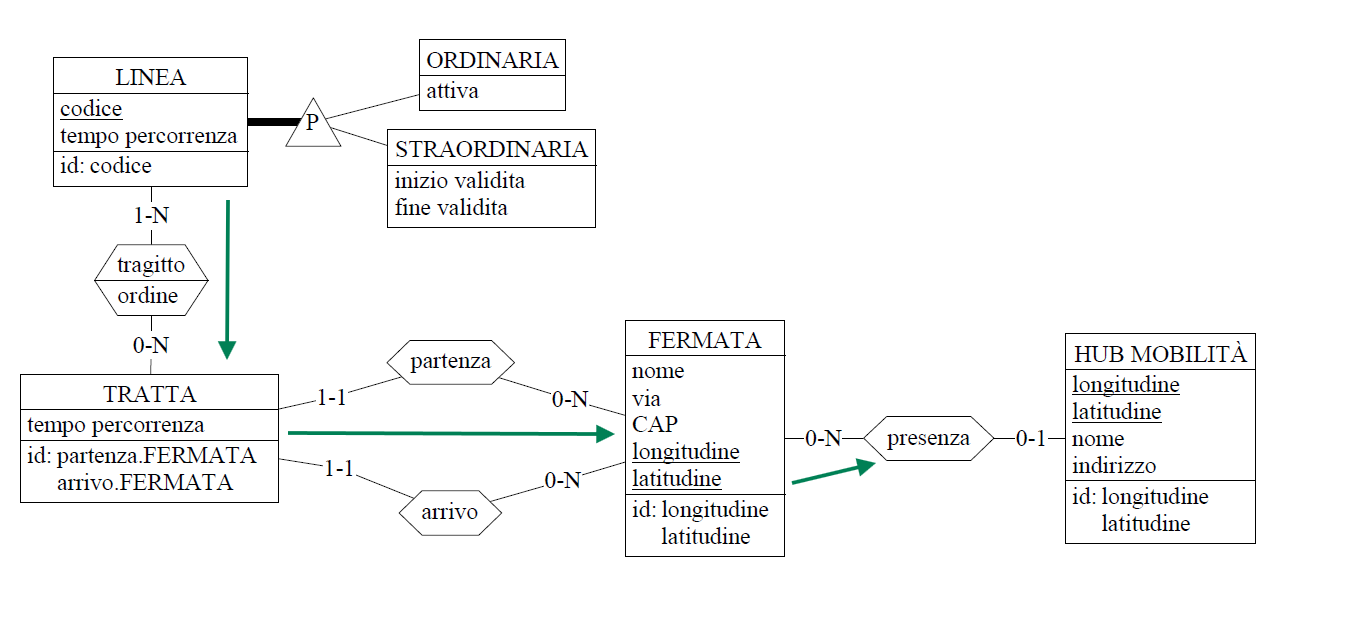
\includegraphics[width=0.9\textwidth]{VisualLineeMaggiorHub}
    \end{center}
    \begin{table}[H]
    \centering
    \begin{tabular}{|c|c|l|l|}
    \hline
    \textbf{Nome} & \textbf{Tipo} & \textbf{Numero accessi} & \textbf{S/L} \\
    \hline
    LINEA & E & 75 & L \\
    \hline
    TRAGITTO & A & 1.500 & L \\
    \hline
    TRATTA & E & 1.000 & L \\
    \hline
    FERMATA & E & 450 & L \\
    \hline
    PRESENZA & A & 165 & L \\
    \hline
    \multicolumn{4}{c}{\textbf{Totale}} \\
    \multicolumn{4}{c}{${A_{lettura}}$ = 3.190, ${A_{scrittura}}$ = 0} \\
    \hline
    \end{tabular}
    \end{table}
    \begin{center}
    ${C_{tot} = {O_{settimana}}\cdot{A_{lettura}}= 9.570}$
    \end{center}

  % -------------------------------------------------------------------------------------------------------------------------------------------
  % -------------------------------------------------------------------------------------------------------------------------------------------

         \item\textbf{Media di soldi spesi in multe per persona} \label{op16} \\
	\[{O_{settimana} = 1}\]
	Questa operazione deve poter essere effettuata dall'amministratore di sistema.\\
	Deve essere estratto un unico numero, ovvero la media del prezzo totale pagato per persona.
	\begin{table}[H]
	\centering
	\begin{tabular}{|l|c|c|c|}
	\hline
	Nome & Tipo & Numero Accessi & S/L \\
	\hline
	MULTA & E & 10000 & L \\
	\hline
	CAUSALE MULTA & E & 10000 & L \\
	    \hline
	    \multicolumn{4}{c}{\textbf{Totale}} \\
	    \multicolumn{4}{c}{${A_{lettura}}$ = 20.000, ${A_{scrittura}}$ = 0} \\
	    \hline
	    \end{tabular}
	    \end{table}
	    \begin{center}
	    ${C_{tot} = {O_{settimana}}\cdot{A_{lettura}}= 20.000}$
	    \end{center}

  % -------------------------------------------------------------------------------------------------------------------------------------------
  % -------------------------------------------------------------------------------------------------------------------------------------------

	\item \textbf{Visualizzazione delle aziende che non hanno effettuato nessuna manutenzione nell’ultimo mese} \label{op17} \\
    \[ {O_{settimana} = 4} \]
    Questa operazione serve a estrarre le aziende che non hanno effettuato nessuna manutenzione nell'ultimo mese.
    \begin{center}
	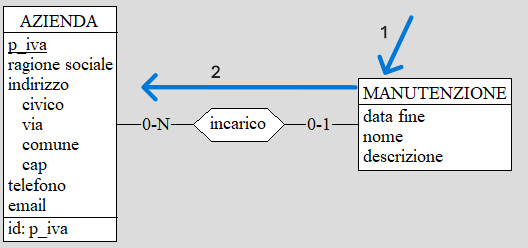
\includegraphics[width=0.7\textwidth]{op_17}
	\end{center}
    \begin{table}[H]
    \centering
    \begin{tabular}{|c|c|l|l|}
    \hline
    \textbf{Nome} & \textbf{Tipo} & \textbf{Numero accessi} & \textbf{S/L} \\
    \hline
    MANUTENZIONE & E & 50 & L \\
    \hline
    AZIENDA & E & x & L \\
    \hline
    \multicolumn{4}{c}{\textbf{Totale}} \\
    \multicolumn{4}{c}{${A_{lettura}}$ = 50 + x, ${A_{scrittura}}$ = 0} \\
    \hline
    \end{tabular}
    \end{table}
    \begin{center}
    ${C_{tot} = {O_{settimana}}\cdot {A_{lettura}} = 200 + 4x}$
    \end{center}

  % -------------------------------------------------------------------------------------------------------------------------------------------
  % -------------------------------------------------------------------------------------------------------------------------------------------

    \item\textbf{Visualizzazione delle fermate in cui è presente almeno un hub mobilità contenente tutti i tipi di servizi green} \label{op18} \\
    \[ {O_{settimana} = 1} \]
    Questa operazione punta a ricercare le fermate più eco-friendly, ovvero che fanno riferimento ad almeno un hub mobilità che contenga TUTTI i tipi di servizi possibili. Si tratta quindi di un'operazione di divisione. \\
    Si vuole quindi visualizzare:
    \begin{itemize}
	\renewcommand\labelitemi{--}
    \item L'elenco dei nomi di tutte le \texttt{FERMATA} che rispettano le specifiche
    \end{itemize}
    \begin{center}
    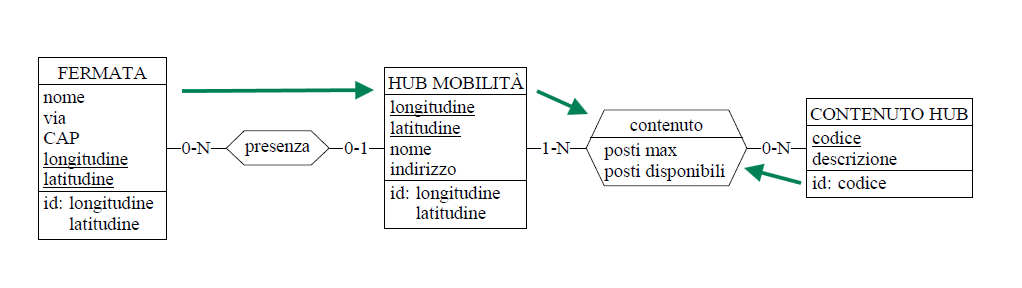
\includegraphics[width=0.8\textwidth]{VisualFermateHubCompleti}
    \end{center}
    \begin{table}[H]
    \centering
    \begin{tabular}{|c|c|l|l|}
    \hline
    \textbf{Nome} & \textbf{Tipo} & \textbf{Numero accessi} & \textbf{S/L} \\
    \hline
    FERMATA & E & 450 & L \\
    \hline
    HUB MOBILITA & E & 225 & L \\
    \hline
    CONTENUTO & A & 450 & L \\
    \hline
    CONTENUTO HUB & E & 4 & L \\
    \hline
    \multicolumn{4}{c}{\textbf{Totale}} \\
    \multicolumn{4}{c}{${A_{lettura}}$ = 1.129, ${A_{scrittura}}$ = 0} \\
    \hline
    \end{tabular}
    \end{table}
    \begin{center}
    ${C_{tot} = {O_{settimana}}\cdot{A_{lettura}}= 1.129}$
    \end{center}


  % -------------------------------------------------------------------------------------------------------------------------------------------
  % -------------------------------------------------------------------------------------------------------------------------------------------
    \item\textbf{Inserimento di una variazione di servizio} \label{op19} \\
	\[{O_{settimana} = 1}\]
	Questa operazione deve poter essere effettuata dall'amministratore di sistema.\\
	Supponendo che le linee straordinarie sostitutive siano già state inserite, si deve creare una nuova manuntenzione.\\
	Alla manuntenzione va indicata la linea che viene modificata, e le eventuali linee che la sostituiscono.\\
	Inoltre se l'inizio della manuntenzione è immediato, allora la linea coinvolta va disattivata.\\
	\textbf{OSS: va calcolato l'impatto di avere o no l'attributo ridondante \texttt{ATTIVA}}

	 \begin{itemize}
            \item \textbf{Analisi con attributo ridondante \texttt{attiva} su \texttt{LINEA}} \\
	\begin{center}
	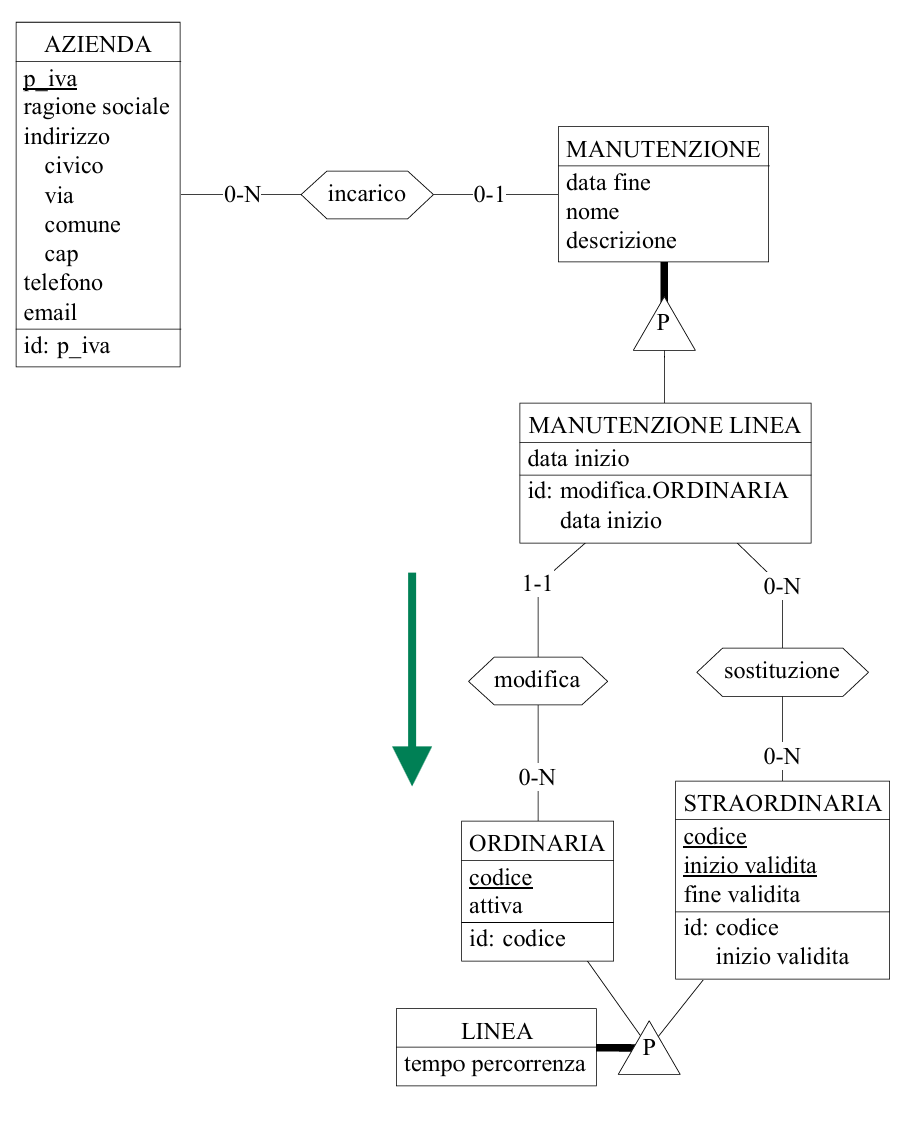
\includegraphics[width=0.6\textwidth]{InserimentoVariazioneServizioRid}
	\end{center}
	\begin{table}[H]
	\centering
	\begin{tabular}{|l|c|c|c|}
	\hline
	Nome & Tipo & Numero Accessi & S/L \\
	\hline
	MANUNTENZIONE LINEA & E & 1 & S \\
	\hline
	ORDINARIA & E & 1 & L \\
	\hline
	ORDINARIA & E & 1 & S \\
	\hline
	SOSTITUZIONE & A & 1 & S \\
	\hline
	    \multicolumn{4}{c}{\textbf{Totale}} \\
	    \multicolumn{4}{c}{${A_{lettura}}$ = 1, ${A_{scrittura}}$ = 3} \\
	    \hline
	    \end{tabular}
	    \end{table}
	    \begin{center}
	    ${C_{tot} = {O_{settimana}}\cdot({A_{lettura}} + {2A_{scrittura}})= 7}$
	    \end{center}

            \item \textbf{Analisi senza attributo ridondante \texttt{attiva} su \texttt{LINEA}} \\
	\begin{center}
	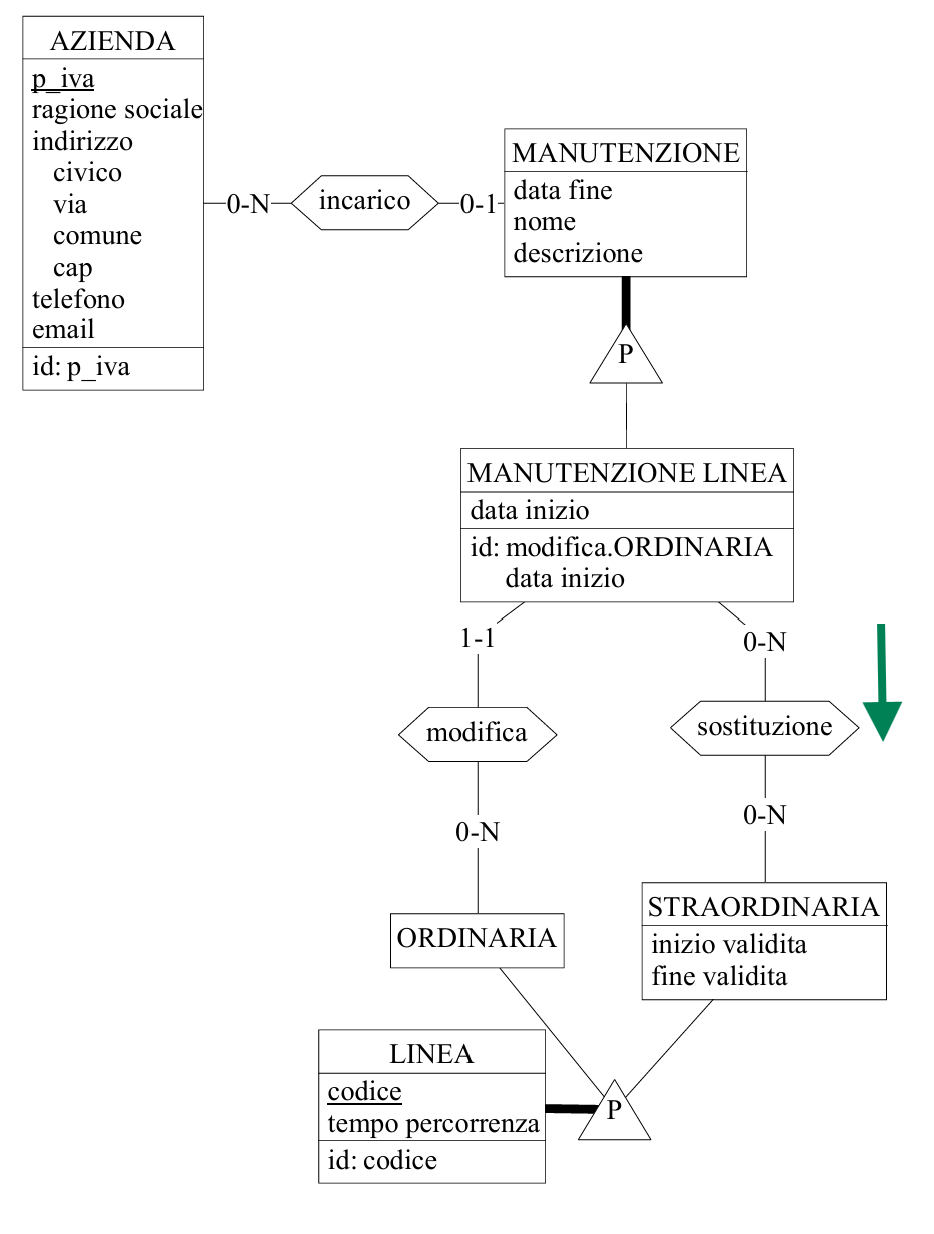
\includegraphics[width=0.8\textwidth]{InserimentoVariazioneServizioNoRid}
	\end{center}
	\begin{table}[H]
	\centering
	\begin{tabular}{|l|c|c|c|}
	\hline
	Nome & Tipo & Numero Accessi & S/L \\
	\hline
	MANUNTENZIONE LINEA & E & 1 & S \\
	\hline
	SOSTITUZIONE & A & 1 & S \\
	\hline
	    \multicolumn{4}{c}{\textbf{Totale}} \\
	    \multicolumn{4}{c}{${A_{lettura}}$ = 0, ${A_{scrittura}}$ = 2} \\
	    \hline
	    \end{tabular}
	    \end{table}
	    \begin{center}
	    ${C_{tot} = {O_{settimana}}\cdot({A_{lettura}} + {2A_{scrittura}})= 4}$
	    \end{center}

	\end{itemize}


  % -------------------------------------------------------------------------------------------------------------------------------------------
  % -------------------------------------------------------------------------------------------------------------------------------------------

    \item\textbf{Aggiunta di una tratta a una linea esistente} \label{op20} \\
    \[ {O_{settimana} = 1} \]
    Questa operazione serve per aggiornare una linea, aggiungendo una fermata al suo tragitto. Nell'analisi terremo conto che la fermata va aggiunta dopo il capolinea, ovvero è necessario solo aggiungere la tratta per poi aggiungerla al traggito. Visto che il tempo di percorrenza di una linea è calcolabile anche come la somma dei tempi di percorrenza delle tratte, si rende necessaria l'analisi differenziata per la presenza dell'attributo \texttt{tempo percorrenza} su \texttt{LINEA}, poiché in caso di ridondanza sarà necessario rieseguire il calcolo del tempo totale per poi aggiornare l'attributo.

    \begin{itemize}
    \item \textbf{Analisi con attributo ridondante \texttt{tempo percorrenza} su \texttt{LINEA}}
    \begin{center}
    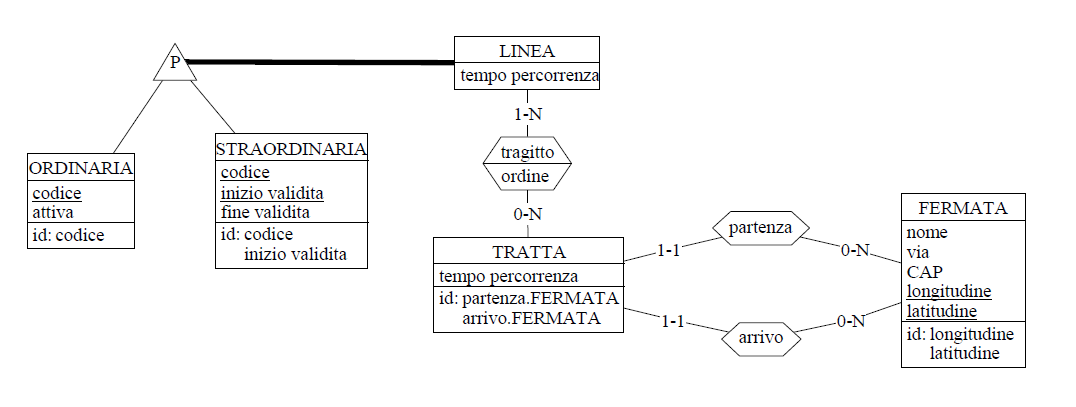
\includegraphics[width=0.8\textwidth]{AggiornaLineaRid}
    \end{center}
    \begin{table}[H]
    \centering
    \begin{tabular}{|c|c|l|l|}
    \hline
    \textbf{Nome} & \textbf{Tipo} & \textbf{Numero accessi} & \textbf{S/L} \\
    \hline
    TRATTA & E & 1 & S \\
    \hline
    TRAGITTO & A & 1 & S \\
    \hline
    TRATTA & A & 21 & L \\
    \hline
    LINEA & E & 1 & S + L \\
    \hline
    \multicolumn{4}{c}{\textbf{Totale}} \\
    \multicolumn{4}{c}{${A_{lettura}}$ = 22, ${A_{scrittura}}$ = 3} \\
    \hline
    \end{tabular}
    \end{table}
    \begin{center}
    ${C_{tot} = {O_{settimana}}\cdot({A_{lettura}} + {2A_{scritttura}})= 28}$
    \end{center}
    \item \textbf{Analisi senza attributo ridondante \texttt{tempo percorrenza} su \texttt{LINEA}}
    \begin{center}
    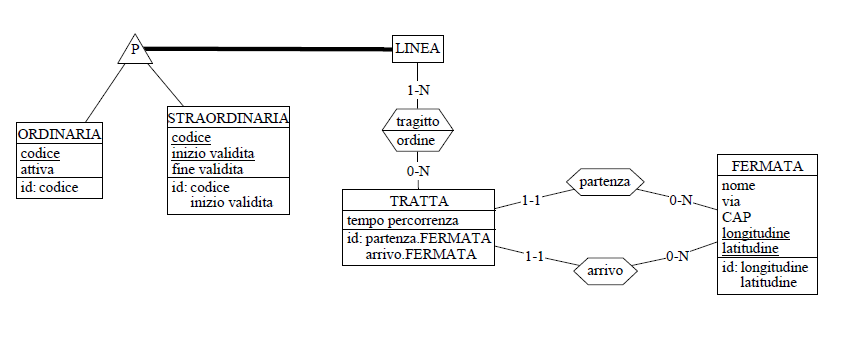
\includegraphics[width=0.8\textwidth]{AggiornaLineaNoRid}
    \end{center}
    \begin{table}[H]
    \centering
    \begin{tabular}{|c|c|l|l|}
    \hline
    \textbf{Nome} & \textbf{Tipo} & \textbf{Numero accessi} & \textbf{S/L} \\
    \hline
    TRATTA & E & 1 & S \\
    \hline
    TRAGITTO & A & 1 & S \\
    \hline
    \multicolumn{4}{c}{\textbf{Totale}} \\
    \multicolumn{4}{c}{${A_{lettura}}$ = 0, ${A_{scrittura}}$ = 2} \\
    \hline
    \end{tabular}
    \end{table}
    \begin{center}
    ${C_{tot} = {O_{settimana}}\cdot{2A_{scritttura}}= 4}$
    \end{center}
    \end{itemize}


  % -------------------------------------------------------------------------------------------------------------------------------------------
  % -------------------------------------------------------------------------------------------------------------------------------------------

    \item\textbf{Creazione di una nuova linea} \label{op21} \\
	\[{O_{settimana} = 1}\]
	Questa operazione deve poter essere fatta dall'amministratore di sistema.\\
	Supponendo che le tratte siano già definite, per ogni linea va indicato l'insieme delle tratte che percorre e, per ogni tratta, specificare l'ordine con cui viene percorsa.\\
	Inoltre vanno sommati i tempi di percorrenza di ogni tratta per calcolare il campo \texttt{tempo percorrenza}

	 \begin{itemize}
    	\item \textbf{Analisi con attributo ridondante \texttt{tempo percorrenza} su \texttt{LINEA}}
	\begin{center}
	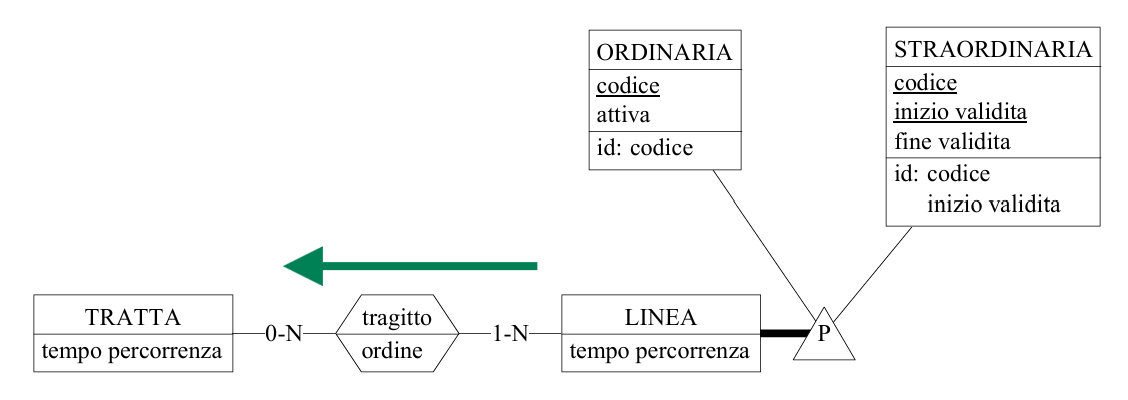
\includegraphics[width=0.7\textwidth]{InserimentoLineaRid}
	\end{center}
	\begin{table}[H]
	\centering
	\begin{tabular}{|l|c|c|c|}
	\hline
	Nome & Tipo & Numero Accessi & S/L \\
	\hline
	LINEA & E & 1 & S \\
	\hline
	TRAGITTO & A & 20 & S \\
	\hline
	TRATTA & E & 20 & L \\
	\hline
	    \multicolumn{4}{c}{\textbf{Totale}} \\
	    \multicolumn{4}{c}{${A_{lettura}}$ = 21, ${A_{scrittura}}$ = 20} \\
	    \hline
	    \end{tabular}
	    \end{table}
	    \begin{center}
	    ${C_{tot} = {O_{settimana}}\cdot{2A_{scritttura}}= 61}$
	    \end{center}

	\item \textbf{Analisi con attributo ridondante \texttt{tempo percorrenza} su \texttt{LINEA}}
	\begin{center}
	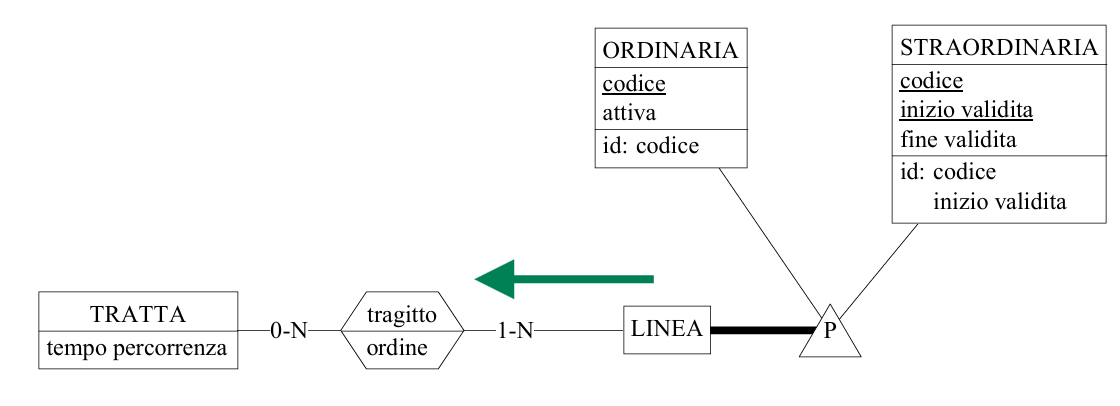
\includegraphics[width=0.7\textwidth]{InserimentoLineaNoRid}
	\end{center}
	\begin{table}[H]
	\centering
	\begin{tabular}{|l|c|c|c|}
	\hline
	Nome & Tipo & Numero Accessi & S/L \\
	\hline
	LINEA & E & 1 & S \\
	\hline
	TRAGITTO & A & 20 & S \\
	\hline
	    \multicolumn{4}{c}{\textbf{Totale}} \\
	    \multicolumn{4}{c}{${A_{lettura}}$ = 1, ${A_{scrittura}}$ = 20} \\
	    \hline
	    \end{tabular}
	    \end{table}
	    \begin{center}
	    ${C_{tot} = {O_{settimana}}\cdot{2A_{scritttura}}= 41}$
	    \end{center}
	\end{itemize}
\end{enumerate}

\section{Analisi delle ridondanze}
In questa sezione andremo ad analizzare le due ridondanze presenti nel modello, ovvero:
\begin{itemize}
  \item \texttt{tempo percorrenza} su \texttt{LINEA}
  \item \texttt{attiva} su \texttt{LINEA}
\end{itemize}

\subsection{Analisi attributo \texttt{tempo percorrenza}}

\begin{table}[H]
	\centering
	\begin{tabular}{|l|c|c|c|}
	\hline
	\textbf{Num Op.} & \textbf{Con ridondanza} & \textbf{Senza ridondanza} \\
	\hline
	4 & 1.153.950 & 12.691.950 \\
  \hline
	5 & 252.200 & 280.200 \\
  \hline
  14 & 150 & 6.150 \\
  \hline
  20 & 28 & 4 \\
  \hline
  21 & 61 & 41 \\
  \hline
  \textbf{TOTALE} & \textbf{1.406.389} & \textbf{12.978.345} \\
  \hline
  \end{tabular}
\end{table}

A fronte di questa analisi, decidiamo di mantenere l'attributo \texttt{tempo percorrenza}.

\subsection{Analisi attributo \texttt{attiva}}

  \begin{table}[H]
  \centering
  \begin{tabular}{|l|c|c|c|}
  \hline
  \textbf{Num Op.} & \textbf{Con ridondanza} & \textbf{Senza ridondanza} \\
  \hline
  1 & 1.950 & 7.800.000 \\
  \hline
  19 & 7 & 4 \\
  \hline
  \textbf{TOTALE} & \textbf{1.957} & \textbf{7.800.004} \\
  \hline
  \end{tabular}
\end{table}

A fronte di questa analisi, decidiamo di mantenere l'attributo \texttt{attiva}.

\section{Riepilogo operazioni}
Nella seguente tabella proponiamo un riepilogo delle operazioni analizzate, con il costo totale per ogni operazione.

\begin{longtable}{|c|p{8cm}|c|l|l|}
\caption{Costo totale delle operazioni stimato per 7 giorni}
\label{table:operazioni_tot}\\
\hline
\textbf{\#} & \textbf{Operazione} & \textbf{Costo tot. / 7gg} & \textbf{Tipo Utente} \\
\hline
\endhead
1  & \hyperref[op1]{Visualizzazione di tutte le linee attive} & 7.800.000 & Tutti \\
\hline
2 & \hyperref[op2]{Visualizzazione fermate e orari di una linea} & 248.500 & Tutti \\
\hline
3 & \hyperref[op3]{Visualizzazione degli hub mobilità} & 645.000 & Tutti \\
\hline
4* & \hyperref[op4]{Visualizzazione orario e mezzo assegnato} & 1.153.950 & Autista \\
\hline
5* & \hyperref[op5]{Visualizzazione orario e linee assegnate} & 252.200 & Controllore \\
\hline
6 & \hyperref[op6]{Estrazione delle linee con più convalide nell'ultimo mese} & 850.005 & Amministratore  \\
\hline
7 & \hyperref[op7]{Estrazione delle manuntenzioni che coinvolgono un determinato mezzo} & 35 & Amministratore \\
\hline
8 & \hyperref[op8]{Estrazione delle manuntenzioni ed eventuali linee sostitutive che coinvolgono una linea} & 205 & Amministratore \\
\hline
9 & \hyperref[op9]{Visualizzazione incassi dati dalle convalide per una linea} & 8.150 & Amministratore \\
\hline
10 & \hyperref[op10]{Estrazione degli incassi per tipo di titolo in periodo definito} & 250.005 & Amministratore \\
\hline
11 & \hyperref[op11]{Estrazione delle linee con più multe in periodo definito} & 503.700 & Amministratore \\
\hline
12 & \hyperref[op12]{Estrazione delle 5 linee con manutenzioni più gravose (in termini linee sostitutive e durata)} & 100 & Amministratore  \\
\hline
13 & \hyperref[op13]{Estrazione delle linee con \textgreater 5 controlli/giorno e \textless = 10 multe/giorno} & 755.100 & Amministratore  \\
\hline
14* & \hyperref[op14]{Visualizzazione delle linee con il maggior tempo di percorrenza} & 150 & Amministratore  \\
\hline
15 & \hyperref[op15]{Estrazione della linea con più hub mobilità lungo il percorso} & 9.570 & Amministratore \\
\hline
16 & \hyperref[op16]{Media di soldi spesi in multe per persona} & 20.000 & Amministratore \\
\hline
17 & \hyperref[op17]{Visualizzazione delle aziende che non hanno effettuato nessuna manutenzione nell'ultimo mese} & 4XXX & Amministratore \\
\hline
18 & \hyperref[op18]{Visualizzazione delle fermate in cui è presente un hub mobilità contenente tutti i tipi di servizi green} & 1.129 & Amministratore \\
\hline
19* & \hyperref[op19]{Inserimento di una variazione di servizio} & 7 & Amministratore \\
\hline
20* & \hyperref[op20]{Aggiunta di una tratta a una linea esistente} & 28 & Amministratore \\
\hline
21* & \hyperref[op21]{Creazione di una nuova linea} & 61 & Amministratore \\
\hline
\end{longtable}

\section{Raffinamento dello schema}
Ora che abbiamo deciso quali attributi dovranno rimanere nella base di dati, non ci resta che apportare dei raffinamenti allo schema ER in modo da rielaborare i concetti non direttamente rappresentabili tramite il modello relazionale.
Procediamo quindi per step successivi fino ad arrivare a uno schema logico equivalente allo schema ER.

\subsection{Rimozione attributi multivalore}
L'unico attributo multivalore nel nostro schema è presente nell'entità \texttt{AZIENDA}, nello specifico l'\texttt{indirizzo}.
Aggiungiamo quindi il prefisso \texttt{indirizzo\textunderscore} a ogni suo componente per poi decomporlo in attributi singoli.

\subsection{Rimozione gerarchie}

\subsubsection{Biglietto}
La gerarchia su biglietto è di tipo Totale ed Esclusiva.
Poiché non ci sono attributi diversi nelle due entità figlie e \texttt{BIGLIETTO DIGITALE} ha l'associazione \texttt{acquisto} di cardinalità (1,1), scegliamo di effettuare un \textbf{collasso vero l'alto}.
L'associazione \texttt{aquisto} diventa quindi a cardinalità (0, 1). \\
Sarà possibile riconoscere i biglietti digitali dai fisici perché questi ultimi non avranno l'associazione \texttt{acquisto} con l'entità \texttt{UTENTE}.

\subsubsection{Titolo di Viaggio}
Anche in questo caso la gerarchia è di tipo Totale ed Esclusiva.
Dal momento che le entità figlie hanno associazioni e attributi diversi, scegliamo di effettuare un \textbf{collasso vero il basso} che ci permette di mantenere questi vincoli inalterati.

\begin{figure}[H]
	\centering
	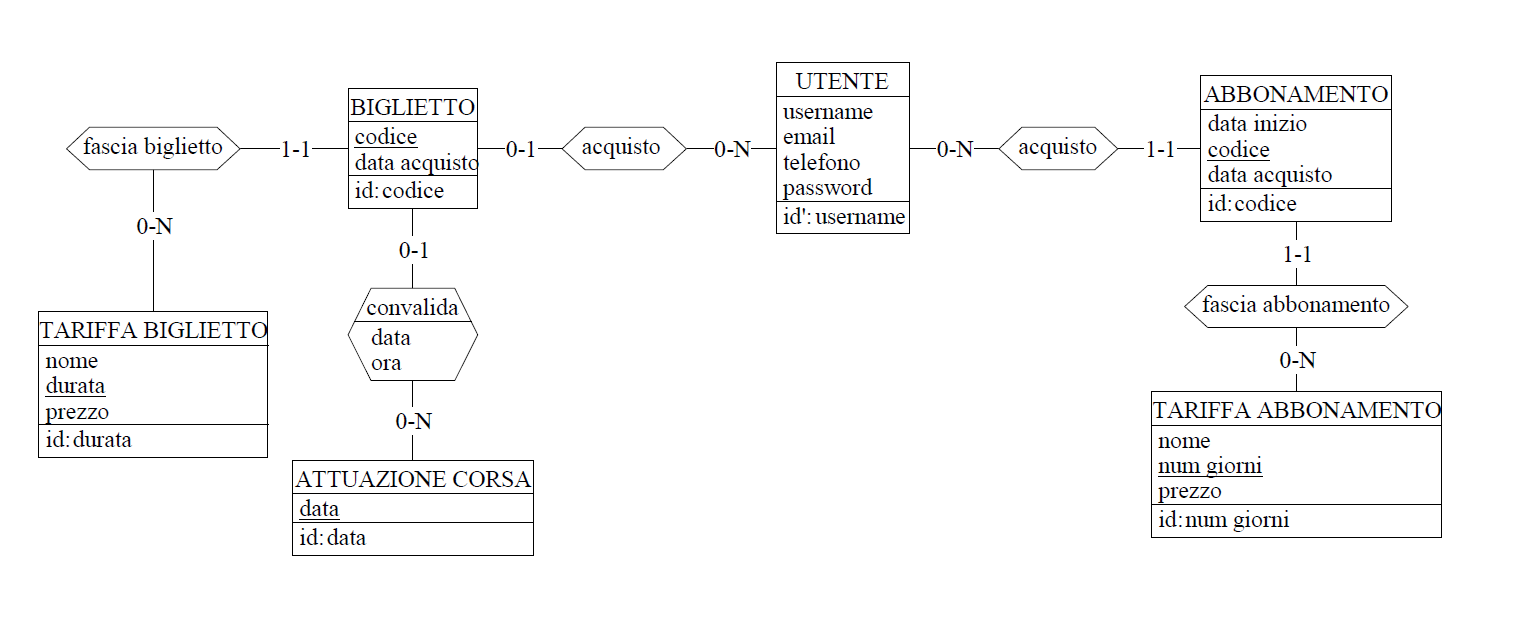
\includegraphics[width=1\textwidth]{GerarchiaTitoloViaggio}
 	\caption{Entità Biglietto e Abbonamento dopo la rimozione delle gerarchie}
\end{figure}

\subsubsection{Persona - Utente}
Abbiamo che \texttt{UTENTE} è un subset di \texttt{PERSONA}.
Se venisse effettuato un collasso avremmo vari attributi opzionali da gestire: scegliamo quindi di sostituire la gerarchia con un'\textbf{associazione}.
Così facendo a una persona fisica può essere connessa un'utenza, e a un'utenza deve per forza essere connessa una persona.

\subsubsection{Utente - Dipendente}
Come per Persona e Utente il subset è stato sostituito dall'associazione \texttt{dipendenza}, visto che le entità \texttt{UTENTE} e \texttt{DIPENDENTE} hanno associazioni diverse.

\subsubsection{Dipendente}
La gerarchia sui vari tipi di dipendente (\texttt{AMMINISTRATIVO}, \texttt{AUTISTA}, \texttt{CONTROLLORE}) è di tipo Totale ed Esclusiva.
Visto che le sottoentità non hanno attributi diversificati, scegliamo di fare un \textbf{collasso verso l'alto}.
Introduciamo un selettore di tipo chiamato \texttt{ruolo} che potrà assumere solo i valori di Amministrativo, Autista o Controllore.
Visto che le associazioni specifiche per ogni ruolo ora fanno riferimento al generico dipendente sarà necessario porre attenzione ad eseguire dei controlli per verificare che si possano aggiungere delle associazioni solo se coerenti con il ruolo del dipendente coinvolto.

\begin{figure}[H]
	\centering
	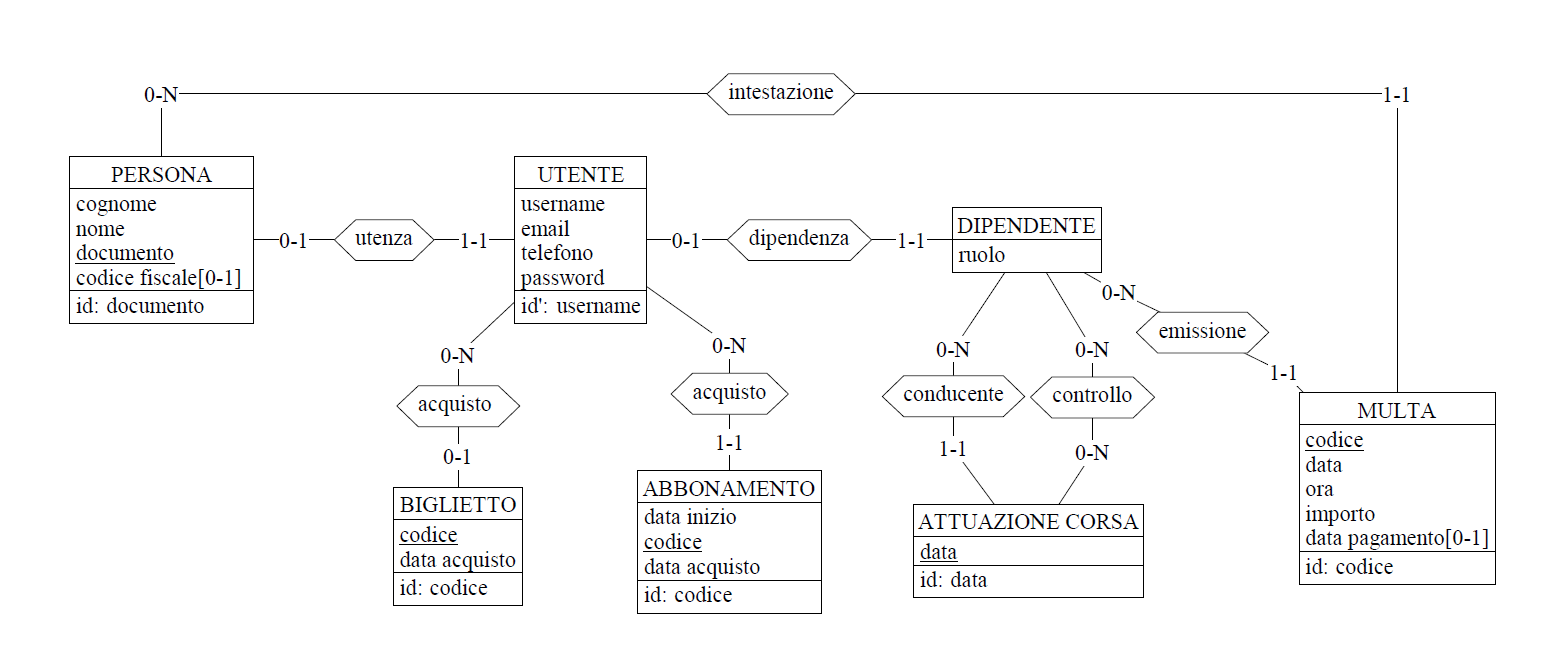
\includegraphics[width=1\textwidth]{GerarchiaPersona}
 	\caption{Entità Persona, Utente e Dipendente dopo la rimozione delle gerarchie}
\end{figure}

\subsubsection{Manutenzione}
La gerarchia su \texttt{MANUTENZIONE} è di tipo Totale ed Esclusiva.
Poiché le due entità figlie si riferiscono a due concetti differenti, quindi hanno anche associazioni diverse, scegliamo di effettuare un \textbf{collasso verso il basso} per mantenere i vincoli sulle associazioni.
Importiamo quindi sui due figli gli attributi comuni e l'associazione comune \texttt{incarico}.

\subsubsection{Linea}
Le linee di tipo ordinario e straordinario compongono una gerarchia Totale ed Esclusiva.
Scegliamo di eseguire un \textbf{collasso verso l'alto}, così da avere tutte le linee in un'unica entità visto che sono oggetto di molte richieste comuni.
Dal momento che hanno alcuni attributi diversi, questi diventeranno degli opzionali e ci serviranno per capire di che tipo è la linea.

\begin{figure}[H]
	\centering
	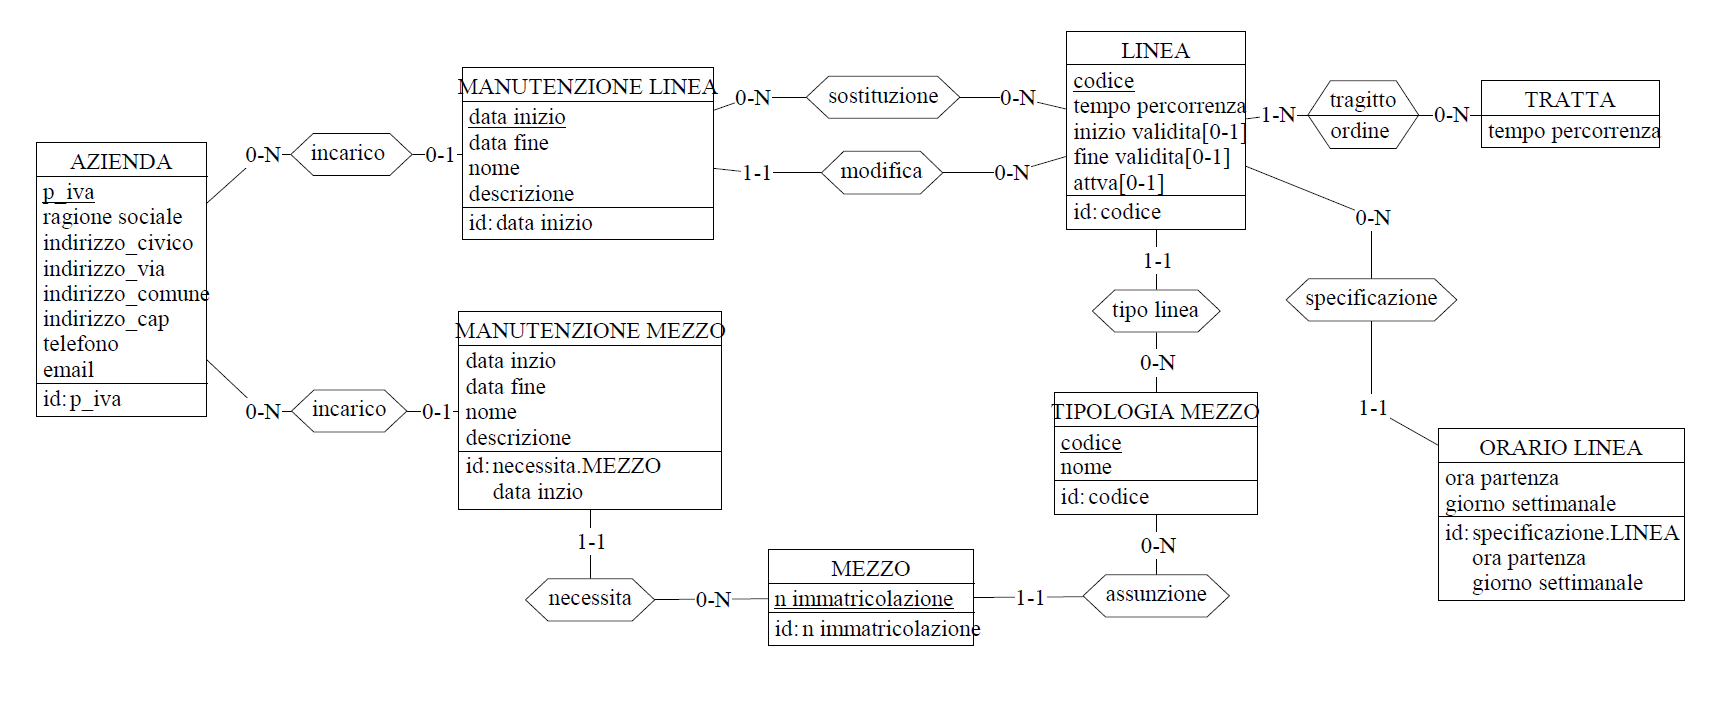
\includegraphics[width=1\textwidth]{GerarchiaLineaManutenzione}
 	\caption{Entità Manutenzione e Linea dopo la rimozione delle gerarchie}
\end{figure}

\subsection{Reificazione associazioni molti a molti}
Le associazioni \texttt{N-N} non sono direttamente rappresentabili nei database relazionali, quindi per ovviare a questo problema, le associazioni subiscono un processo di \textbf{reificazione} che comporta la trasformazione dell'associazione \texttt{N-N} in un'entità che sarà connessa con due associazioni \texttt{1-1} alle entità che prima collegava.\\ \\
Qui elencate troviamo le associazioni che sono state reificate:
\begin{itemize}
    \item Contenuto
    \item Tragitto
    \item Sostituzione
    \item Controllo
\end{itemize}

\subsection{Scelta degli identificatori principali}
Tutte le entità del nostro dominio sono già dotate dei loro identificatori principali naturali.
Per comodità ne sostituiamo alcuni con un semplice codice (lasciando comunque il vincolo di unicità su quelli esistenti) per rendere più semplici le query.\\
Riportiamo l'elenco delle entità in cui è stata effettuata quest'aggiunta:
\begin{itemize}
    \item Fermata
    \item Hub mobilità
    \item Orario linea
    \item Causale multa
    \item Attuazione Corsa
\end{itemize}

\section{Schema relazionale finale}\label{section:schema_relazionale}
A questo punto la ristrutturazione è terminata, e il nostro schema è direttamente traducibile in delle relazioni.
Riportiamo nelle pagine seguenti lo schema logico sia in formato grafico che testuale.

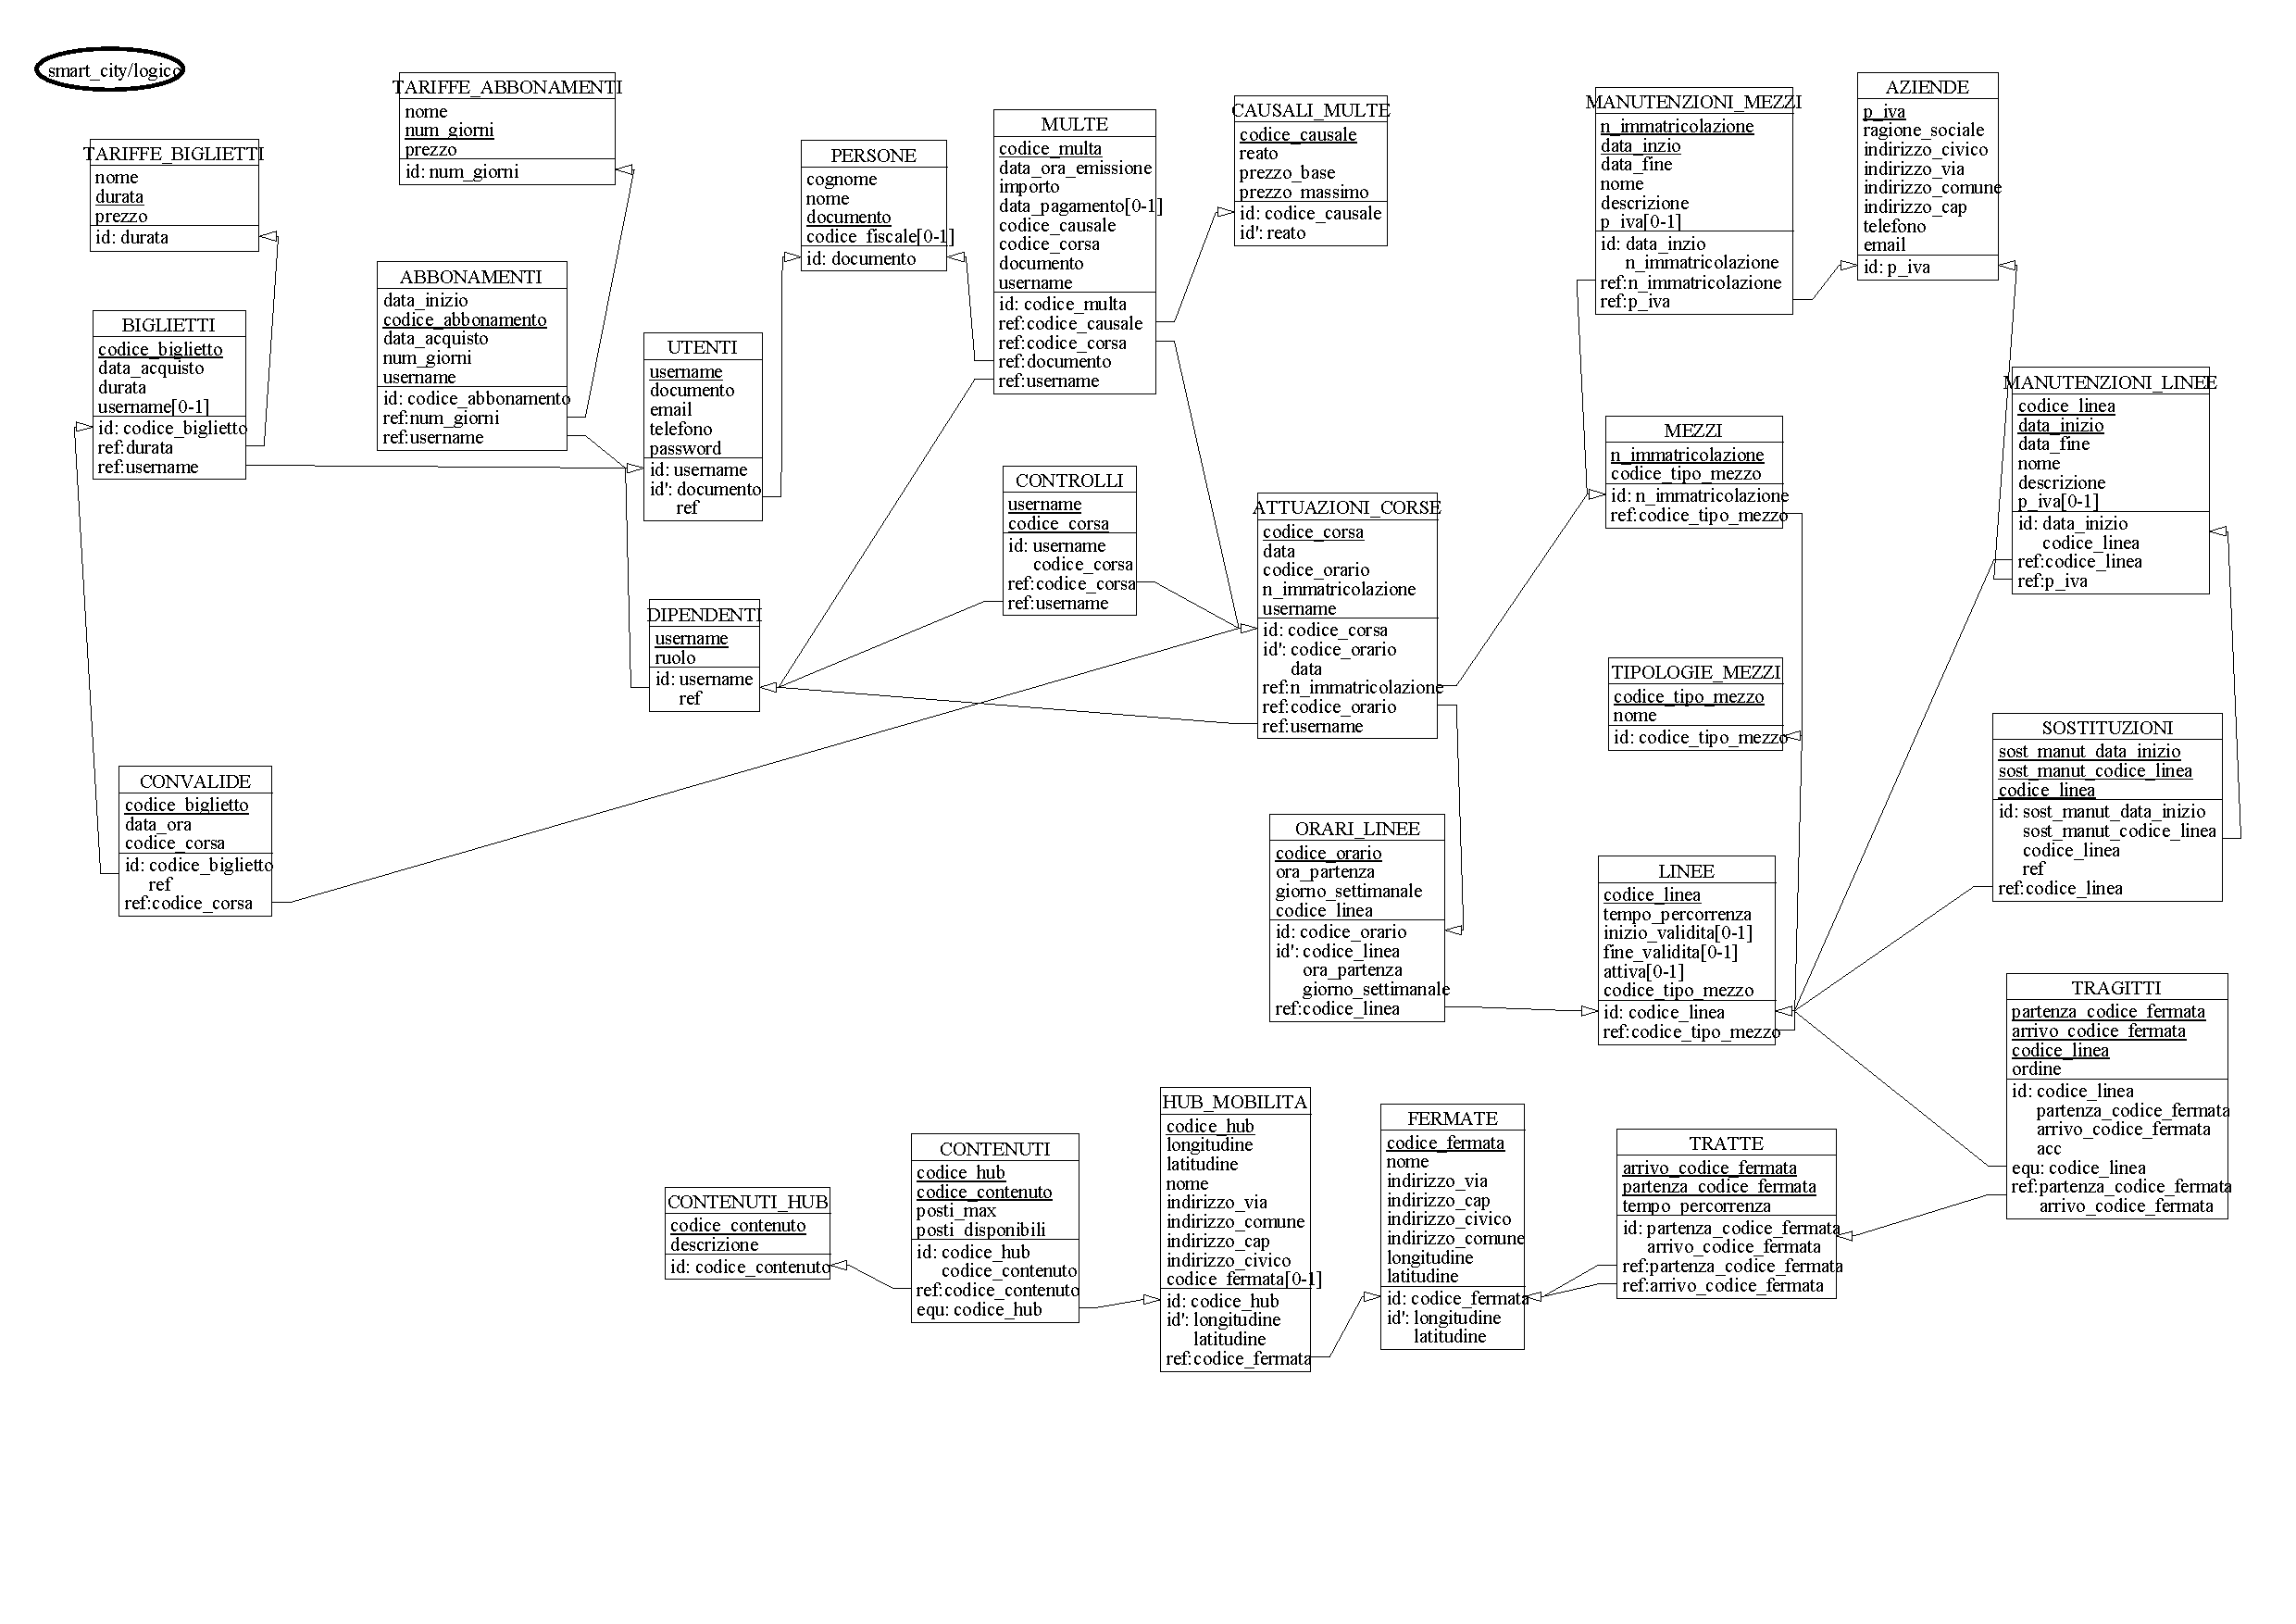
\includepdf{src/pdf/Schema_Logico.pdf}

\begin{itemize}
\item\texttt{
    \textbf{PERSONE}(\underline{documento}, cognome, nome, codice\_fiscale*)
}
\item\texttt{
    \textbf{UTENTI}(\underline{username}, documento: PERSONE, email, telefono, password)\\
    UNIQUE: (documento)
}
\item\texttt{
    \textbf{DIPENDENTI}(\underline{username}: UTENTI, ruolo)
}
\item\texttt{
     \textbf{FERMATE}(\underline{codice\_fermata}, nome, indirizzo\_via, indirizzo\_cap, \\indirizzo\_civico, indirizzo\_comune, longitudine, latitudine) \\
     UNIQUE: (longitudine, latitudine)
}
\item\texttt{
    \textbf{HUB\_MOBILITA}(\underline{codice\_hub}, longitudine, latitudine, nome, indirizzo\_via, indirizzo\_comune, indirizzo\_cap,  indirizzo\_civico, codice\_fermata*: FERMATE)\\
    UNIQUE: (longitudine, latutudine)
}
\item\texttt{
    \textbf{CONTENUTI\_HUB}(\underline{codice\_contenuto}, descrizione)
}
\item\texttt{
    \textbf{CONTENUTI}(\underline{codice\_hub}: HUB\_MOBILITA, \underline{codice\_contenuto}: CONTENUTI\_HUB, posti\_max, posti\_disponibili)
}
\item\texttt{
    \textbf{TRATTE}(\underline{partenza\_codice\_fermata}: FERMATE, \underline{arrivo\_codice\_fermata}: FERMATE, tempo\_percorrenza)
}
\item\texttt{
    \textbf{TRAGITTI}((\underline{partenza\_codice\_fermata}, \underline{arrivo\_codice\_fermata}): TRATTE, \\\underline{codice\_linea}:LINEE, ordine)
}
\item\texttt{
    \textbf{TIPOLOGIE\_MEZZI}(\underline{codice\_tipo\_mezzo}, nome)
}
\item\texttt{
    \textbf{MEZZI}(\underline{n\_immatricolazione}, codice\_tipo\_mezzo: TIPOLOGIE\_MEZZI)
}
\item\texttt{
    \textbf{LINEE}(\underline{codice\_linea}, tempo\_percorrenza, inizio\_validita*, fine\_validita*, attiva*, codice\_tipo\_mezzo: TIPOLOGIE\_MEZZI)
}
\item\texttt{
    \textbf{ORARI\_LINEE}(\underline{codice\_orario}, ora\_partenza, giorno\_settimanale, \\codice\_linea: LINEE) \\
    UNIQUE: (codice\_linea, ora\_partenza, giorno\_settimanale)
}
\item\texttt{
    \textbf{ATTUAZIONI\_CORSE}(\underline{codice\_corsa}, data, codice\_orario: ORARI\_LINEE, \\n\_immatricolazione: MEZZI, username: DIPENDENTI)\\
    UNIQUE: (codice\_orario, data)
}
\item\texttt{
    \textbf{CAUSALI\_MULTE}(\underline{codice\_causale}, reato, prezzo\_base, prezzo\_massimo)\\
    UNIQUE: (reato)
}
\item\texttt{
    \textbf{MULTE}(\underline{codice\_multa}, data\_ora\_emissione, importo, data\_pagamento*, \\codice\_causale: CAUSALI\_MULTE, codice\_corsa: ATTUAZIONI\_CORSE, \\documento: PERSONE, username: DIPENDENTI)
}
\item\texttt{
    CONTROLLI(\underline{username}: DIPENDENTI, \underline{codice\_corsa}: ATTUAZIONI\_CORSE)
}
\item\texttt{
    \textbf{TARIFFE\_BIGLIETTI}(\underline{durata}, nome, prezzo)
}
\item\texttt{
    \textbf{BIGLIETTI}(\underline{codice\_biglietto}, data\_acquisto, durata: TARIFFE\_BIGLIETTI, username*: UTENTI)
}
\item\texttt{
    \textbf{CONVALIDE}(\underline{codice\_biglietto}: BIGLIETTI, data\_ora, \\codice\_corsa: ATTUAZIONI\_CORSE)
}
\item\texttt{
    \textbf{TARIFFE\_ABBONAMENTI}(\underline{num\_giorni}, nome, prezzo)
}
\item\texttt{
    \textbf{ABBONAMENTI}(\underline{codice\_abbonamento}, num\_giorni: TARIFFE\_ABBONAMENTI, \\data\_inizio, data\_acquisto, username: UTENTI)
}
\item\texttt{
    \textbf{AZIENDE}(\underline{p\_iva}, ragione\_sociale, indirizzo\_civico, indirizzo\_via, \\indirizzo\_comune, indirizzo\_cap, telefono, email)
}
\item\texttt{
    \textbf{MANUTENZIONE\_MEZZI}(\underline{n\_immatricolazione}: MEZZI, \underline{data\_inizio}, data\_fine, nome, descrizione, p\_iva*: AZIENDE)
}
\item\texttt{
    \textbf{MANUTENZIONI\_LINEE}(\underline{codice\_linea}: LINEE, \underline{data\_inizio}, data\_fine, nome, descrione, p\_iva*: AZIENDE)
}
\item\texttt{
    \textbf{SOSTITUZIONI}(\\(\underline{sost\_manut\_data\_inizio}, \underline{sost\_manut\_codice\_linea}): \ MANUNTENZIONI\_LINEE, \\\underline{codice\_linea}: LINEE)
}
\end{itemize}

\chapter{Progettazione della Base di Dati}\label{chapter:db}

Abbiamo creato la base di dati per il nostro applicativo mappando le relazioni (vedi \cref{section:schema_relazionale}) in tabelle, utilizzando il DBMS \textbf{MySQL}. Per eseguire la traduzione abbiamo sfruttato lo strumento messo a disposizione da \texttt{DB-Main}. \\
Riportiamo in seguito il codice per eseguire ogni operazione indicata in \cref{table:operazioni}, e le altre peculiarità relative alla creazione del database.

\section{Check}
Nella creazione delle tabelle abbiamo inserito vari check, per poter definire meglio il dominio dei dati inseribili nel database. \\

\begin{lstlisting}[style=sqlstyle, caption=Esempio di check utilizzato per definire gli attributi \texttt{prezzo} e \texttt{durata} come numeri positivi.]
create table TARIFFE_BIGLIETTI (
     nome varchar(30) not null,
     durata int not null,
     prezzo decimal(6,2) not null,
     check (durata > 0 and prezzo > 0),
     constraint ID_TARIFFA_BIGLIETTO primary key (durata));
\end{lstlisting}

\section{Viste}
Visto che l'operazione di visualizzazione delle linee attive nel giorno corrente ricopre un ruolo centrale nel nostro applicativo, abbiamo deciso di creare una vista che estrae tutte le linee attive (sia ordinarie che straordinarie) riportando anche la prima e l'ultima fermata del tragitto complessivo. \\
\begin{lstlisting}[style=sqlstyle, label=code:lines_view, caption=Codice SQL per la creazione della vista]
CREATE VIEW VW_LINEE_ATTIVE_OGGI AS
SELECT L.*, M.nome AS tipo_mezzo, F1.codice_fermata AS part_codice_fermata, F1.nome AS part_nome, F1.indirizzo_via AS part_via, F1.indirizzo_civico AS part_civico, F1.indirizzo_comune AS part_comune, F1.indirizzo_cap AS part_cap, F1.longitudine AS part_long, F1.latitudine AS part_lat, F2.codice_fermata AS arr_codice_fermata, F2.nome AS arr_nome, F2.indirizzo_via AS arr_via, F2.indirizzo_civico AS arr_civico, F2.indirizzo_comune AS arr_comune, F2.indirizzo_cap AS arr_cap, F2.longitudine AS arr_long, F2.latitudine AS arr_lat
FROM LINEE L
JOIN TIPOLOGIE_MEZZI M ON L.codice_tipo_mezzo = M.codice_tipo_mezzo
JOIN TRAGITTI TRA1 on TRA1.codice_linea = L.codice_linea
JOIN TRATTE TR1 ON (TRA1.partenza_codice_fermata = TR1.partenza_codice_fermata AND TRA1.arrivo_codice_fermata = TR1.arrivo_codice_fermata)
JOIN FERMATE F1 ON F1.codice_fermata = TR1.partenza_codice_fermata
JOIN TRAGITTI TRA2 on TRA2.codice_linea = L.codice_linea
JOIN TRATTE TR2 ON (TRA2.partenza_codice_fermata = TR2.partenza_codice_fermata AND TRA2.arrivo_codice_fermata = TR2.arrivo_codice_fermata)
JOIN FERMATE F2 ON F2.codice_fermata = TR2.arrivo_codice_fermata
WHERE TRA1.ordine = 1
    AND TRA2.ordine =
        (SELECT MAX(T1.ordine)
        FROM LINEE L1 JOIN TRAGITTI T1 ON L1.codice_linea = T1.codice_linea
        WHERE L1.codice_linea = L.codice_linea)
            AND (L.attiva IS TRUE OR (CURDATE() BETWEEN L.inizio_validita AND L.fine_validita)
        )
ORDER BY L.codice_linea;
\end{lstlisting}

\section{Stored Procedures}
L'introduzione della ridondanza sull'attributo \texttt{attiva} delle linee ordinarie ne rende necessaria la sua gestione (attivazione e disattivazione). Per rendere più semplice questa operazione, abbiamo creato due stored procedures:
\begin{itemize}
	\item La prima prende il codice di una linea e controlla che non ci sia attualmente nessuna manutenzione per la linea data
	\item La seconda esegue l'operazione per tutte le linee ordinarie, sfruttando la procedura precedente
\end{itemize}

\begin{lstlisting}[style=sqlstyle]
DELIMITER //

CREATE PROCEDURE aggiorna_attivazione_linea(IN cod_linea VARCHAR(30))
BEGIN
    UPDATE linee L
    SET attiva = NOT EXISTS
        (SELECT 1
	FROM manutenzioni_linee
	WHERE codice_linea = cod_linea AND CURDATE() BETWEEN data_inizio AND data_fine)
    WHERE codice_linea = cod_linea;
END //

DELIMITER ;
\end{lstlisting}

\begin{lstlisting}[style=sqlstyle]
DELIMITER //

CREATE PROCEDURE aggiorna_attivazione_linee()
BEGIN
    DECLARE done INT DEFAULT FALSE;
    DECLARE cur_cod_linea VARCHAR(30);

    DECLARE cur CURSOR FOR
        SELECT codice_linea FROM linee WHERE attiva IS NOT NULL;

    DECLARE CONTINUE HANDLER FOR NOT FOUND SET done = TRUE;

    OPEN cur;

    read_loop: LOOP
        FETCH cur INTO cur_cod_linea;
        IF done THEN
            LEAVE read_loop;
        END IF;
        CALL aggiorna_attivazione_linea(cur_cod_linea);
    END LOOP;

    CLOSE cur;
END //

DELIMITER ;
\end{lstlisting}

\section{Trigger}
Per rendere automatica la gestione della ridondanza dell'attributo \texttt{attiva}, ogni volta che viene effettuata un'operazione che modifica la tabella \texttt{MANUTENZIONI{\textunderscore}LINEE} viene richiamata la stored procedure per aggiornare l'attributo della linea modificata sfruttando dei trigger. Questo permette agli utilizzatori del database di gestire le manutenzioni senza preoccuparsi di tenere aggiornato l'attributo \texttt{attiva}. \\
\begin{lstlisting}[style=sqlstyle]
DELIMITER //

CREATE TRIGGER dopo_insert_manut_linea
AFTER INSERT ON manutenzioni_linee
FOR EACH ROW
BEGIN
    CALL aggiorna_attivazione_linea(NEW.codice_linea);
END//

CREATE TRIGGER dopo_update_manut_linea
AFTER UPDATE ON manutenzioni_linee
FOR EACH ROW
BEGIN
    CALL aggiorna_attivazione_linea(NEW.codice_linea);
END//

CREATE TRIGGER dopo_delete_manut_linea
AFTER DELETE ON manutenzioni_linee
FOR EACH ROW
BEGIN
    CALL aggiorna_attivazione_linea(OLD.codice_linea);
END//

DELIMITER ;
\end{lstlisting}

\section{Eventi}
Le manutenzioni delle linee possono terminare in una data qualasiasi registrata al momento dell'inserimento della manutenzione stessa: ad esempio oggi potrebbe essere terminata la manutenzione della linea 2, ma nessuno potrebbe essersi ricordato di riattivare la linea. Diventa quindi necessario eseguire ogni giorno il "refresh" di tutte le linee attive nel giorno corrente. Questa operazione viene eseguita sfruttando un evento MySQL, che invoca una volta al giorno la stored procedure adibita all'aggiornamento dell'attributo \texttt{attiva} su tutte le linee ordinarie. \\
\begin{lstlisting}[style=sqlstyle]
CREATE EVENT aggiorna_linee_event
ON SCHEDULE EVERY 1 DAY
DO
  CALL aggiorna_attivazione_linee();
\end{lstlisting}

\section{Traduzione delle operazioni in query SQL}
Nelle query potrebbero apparire dei simboli \texttt{?}: questo perché abbiamo utilizzato i prepared statement per poter adattare le clausole where ai filtri imposti dagli utenti.

\begin{enumerate}[label=\textbf{\arabic*)}]

\item \textbf{Visualizzazione di tutte le linee attive} \\
Quest'operazione corrisponde alla visualizzazione delle informazioni estratte dalla vista indicata nel \autoref{code:lines_view}. Sfruttiamo quindi la vista senza dover riscrivere la query.\\
\begin{lstlisting}[style=sqlstyle]
SELECT *
FROM VW_LINEE_ATTIVE_OGGI;
\end{lstlisting}

\item \textbf{Visualizzazione fermate e orari di una linea} \\
Questa operazione è stata divisa in 2 parti dato che sulla UI non mostreremo mai tutte le fermate con i relativi orari di ogni linea; ma mostreremo tutte le linee poi l'utente potrà visualizzare le fermate e gli orari della linea desiderata.
\begin{lstlisting}[style=sqlstyle, caption=Query for Fermate Details by Linea]
SELECT t.codice_linea, t.arrivo_codice_fermata, t.partenza_codice_fermata, t.ordine, f.nome, f.indirizzo_via, f.indirizzo_civico, f.indirizzo_comune, f.indirizzo_cap, tr.tempo_percorrenza
FROM TRAGITTI t
JOIN TRATTE tr ON t.partenza_codice_fermata = tr.partenza_codice_fermata
AND t.arrivo_codice_fermata = tr.arrivo_codice_fermata
JOIN FERMATE f ON t.arrivo_codice_fermata = f.codice_fermata
WHERE t.codice_linea = ?
\end{lstlisting}

\begin{lstlisting}[style=sqlstyle, caption=Query for Orari Linee with Attuazioni Corse]
SELECT ol.codice_orario, ol.codice_linea, ol.orario_partenza, ol.giorno_settimanale, ac.data
FROM ORARI_LINEE ol
JOIN ATTUAZIONI_CORSE ac ON ol.codice_orario = ac.codice_orario
WHERE ol.codice_linea = ?
\end{lstlisting}

\item \textbf{Visualizzazione degli hub mobilità} \\
\begin{lstlisting}[style=sqlstyle, caption=Query for Hub Mobilità with Contenuti and Fermate]
SELECT h.codice_hub, h.nome nome_hub, h.indirizzo_via, h.indirizzo_civico, h.indirizzo_comune, h.indirizzo_cap, h.longitudine, h.latitudine, h.codice_fermata, f.nome nome_fermata, ch.descrizione tipo_contenuto, c.posti_disponibili
FROM HUB_MOBILITA h LEFT JOIN FERMATE f on (h.codice_fermata = f.codice_fermata)
JOIN CONTENUTI c ON (c.codice_hub = h.codice_hub)
JOIN CONTENUTI_HUB ch ON (c.codice_contenuto = ch.codice_contenuto)
ORDER BY h.codice_hub;
\end{lstlisting}

\item \textbf{Visualizzazione orario e linee assegnate agli autisti} \\
Con questa operazione andiamo a visualizzare l'orario di lavoro di un autista e il mezzo che gli è stato assegnato per le linee che dovrà percorrere. Le ore effettive di lavoro potranno essere visualizzare tramite il tempo di percorrenza delle linee che dovrà percorrere.
\begin{lstlisting}[style=sqlstyle, caption=Query for Corse Attuate by User]
SELECT ol.codice_linea, ol.ora_partenza, ol.giorno_settimanale, ol.codice_orario, ac.data,l.tempo_percorrenza, ac.n_immatricolazione
FROM ORARI_LINEE ol
JOIN ATTUAZIONI_CORSE ac ON ol.codice_orario = ac.codice_orario
JOIN LINEE l ON ol.codice_linea = l.codice_linea
WHERE ac.username = ?
ORDER BY ac.data, ol.ora_partenza;
\end{lstlisting}

\item \textbf{Visualizzazione orario e linee assegnate ai controllori} \\
\begin{lstlisting}[style=sqlstyle]
SELECT A.data, O.codice_orario, O.ora_partenza, O.giorno_settimanale, O.codice_linea, L.tempo_percorrenza, A.n_immatricolazione
FROM CONTROLLI C
JOIN ATTUAZIONI_CORSE A ON C.codice_corsa = A.codice_corsa
JOIN ORARI_LINEE O ON A.codice_orario = O.codice_orario
JOIN LINEE L ON O.codice_linea = L.codice_linea
WHERE C.username = ?
ORDER BY A.data, O.ora_partenza;
\end{lstlisting}

\item \textbf{Estrazione delle linee con più convalide nell’ultimo mese} \\
Con questa operazione andremo ad estrarre il numero di convalide per linea in ordine decrescente.
\begin{lstlisting}[style=sqlstyle, caption=Query for Number of Validations per Linea]
SELECT COUNT(*) AS numero_convalide
FROM LINEE l
JOIN ORARI_LINEE ol ON l.codice_linea = ol.codice_linea
JOIN ATTUAZIONI_CORSE ac ON ol.codice_orario = ac.codice_orario
JOIN CONVALIDE c ON ac.codice_corsa = c.codice_corsa
GROUP BY codice_linea
ORDER BY COUNT(*) DESC
\end{lstlisting}

\item \textbf{Estrazione delle manuntenzioni che coinvolgono un determinato mezzo} \\
\begin{lstlisting}[style=sqlstyle]
SELECT *
FROM MANUTENZIONI_MEZZI mm
WHERE mm.n_immatricolazione = ?
\end{lstlisting}

\item \textbf{Estrazione delle manuntenzioni ed eventuali linee sostitutive che coinvolgono una linea (Variazioni di servizio)*} \\
\begin{lstlisting}[style=sqlstyle, caption=Query for Linee in Manutenzione and Their Sostituzioni]
SELECT l.codice_linea codice_linea_in_manutenzione, m.data_inizio, m.data_fine, m.nome, m.descrizione, a.p_iva, a.email, a.telefono, a.ragione_sociale, ls.codice_linea codice_linea_sostituta
FROM LINEE l JOIN MANUTENZIONI_LINEE m ON (m.codice_linea = l.codice_linea)
LEFT JOIN AZIENDE a ON (m.p_iva = a.p_iva)
LEFT JOIN SOSTITUZIONI s ON (m.codice_linea = s.sost_manut_codice_linea AND m.data_inizio = s.sost_manut_data_inizio)
JOIN LINEE ls ON (ls.codice_linea = s.codice_linea)
WHERE l.codice_linea = ?;
\end{lstlisting}

\item \textbf{Visualizzazione incassi dati dalle convalide per una linea} \\
\begin{lstlisting}[style=sqlstyle, caption=Query for Total Revenue (Incassi) by Linea]
SELECT sum(tb.prezzo) AS incassi
FROM ORARI_LINEE ol
JOIN ATTUAZIONI_CORSE ac ON ol.codice_linea = ac.codice_linea
JOIN CONVALIDE c ON ac.codice_corsa = c.codice_corsa
JOIN BIGLIETTI b ON c.codice_biglietto = b.codice_biglietto
JOIN TARIFFE_BIGLIETTI tb ON b.durata = tb.durata
WHERE ol.codice_linea = ?
\end{lstlisting}

\item \textbf{Estrazione degli incassi per tipo di tariffa dei biglietti in periodo definito} \\
Utilizziamo la funzione DATE() per trasformare l'attributo \texttt{data{\textunderscore}ora} da tipo DATETIME a tipo DATE. \\
\begin{lstlisting}[style=sqlstyle]
SELECT SUM(prezzo) as incasso
FROM CONVALIDE C
JOIN BIGLIETTI B ON C.codice_biglietto = B.codice_biglietto
JOIN TARIFFE_BIGLIETTI T ON B.durata = T.durata
WHERE B.durata = ? AND (DATE(C.data_ora) BETWEEN ? AND ?);
\end{lstlisting}

\item \textbf{Estrazione delle linee con più multe in periodo definito} \\
\begin{lstlisting}[style=sqlstyle, caption=Query for Number of Fines per Linea Between Two Dates]
SELECT l.codice_linea, COUNT(*) numero_multe
FROM LINEE l, ORARI_LINEE ol, ATTUAZIONI_CORSE ac, MULTE m
WHERE l.codice_linea = ol.codice_linea
AND ol.codice_orario = ac.codice_orario
AND ac.codice_corsa = m.codice_corsa
AND ac.data BETWEEN ? AND ?
GROUP BY l.codice_linea
ORDER BY numero_multe DESC;
\end{lstlisting}

\item \textbf{Estrazione delle 5 linee con manutenzioni più gravose (in termini di linee sostitutive e durata)} \\
Dobbiamo visualizzare le linee con le manutenzioni più gravose; la gravità verrà calcolata tramite un punteggio che indicherà quanto siano "pesanti" le manutenzioni:
	    \begin{itemize}
		\renewcommand\labelitemi{--}
	        \item +5 pti ogni linea straordinaria dovuta alla manutenzione
	        \item +1 pto ogni 3 giorni di lavoro sulla  linea.
	    \end{itemize}
\begin{lstlisting}[style=sqlstyle, caption=Query for Duration of Maintenance and Substitute Lines Count]
SELECT ml.codice_linea, ml.nome, DATEDIFF(ml.data_fine, ml.data_inizio) AS durata_lavoro, COUNT(*) AS num_linee_sostitutive
FROM MANUTENZIONI_LINEE ml
JOIN SOSTITUZIONI s ON ml.codice_linea = s.sost_manut_codice_linea
GROUP BY ml.codice_linea, ml.data_inizio, ml.nome
\end{lstlisting}

\item \textbf{Estrazione delle linee con \textgreater 5 controlli/giorno e \textless = 10 multe/giorno} \\
Lo scopo è quello di estrarre le linee che in tutti i giorni in cui sono state effettuate attuazioni corsa, sono stati svolti 5 controlli e 10 multe.
La query è stata divisa in 2 subquery:
\begin{itemize}
  \item Nella query più interna vengono selezionati i giorni in cui la condizione $ controlli > 5  \cap multe \leq 10  $ è rispettata
  \item Nella query di mezzo vengono contate quante sono le attuazioni corsa effettuate nei giorni che rispettano la condizione
\end{itemize}
Alla fine vengono contate le attuazioni corsa totali di una linea e vengono confrontate con il numero di attuazioni corsa contate dalla subquery di mezzo. Se sono lo stesso numero (ovvero tutte le attuazioni corsa rispettano la condizione) allora la linea viene visualizzata.
\begin{lstlisting}[style=sqlstyle, caption=Query to Find Lines Matching Fine/Control Conditions on All Trips]
SELECT DISTINCT l.codice_linea
FROM LINEE l JOIN ORARI_LINEE ol ON (l.codice_linea = ol.codice_linea)
JOIN ATTUAZIONI_CORSE ac ON (ol.codice_orario = ac.codice_orario)
GROUP BY l.codice_linea
HAVING COUNT(DISTINCT ac.codice_corsa) = (SELECT COUNT(DISTINCT ac1.codice_corsa)
    FROM LINEE l1 JOIN ORARI_LINEE ol1 ON (l1.codice_linea = ol1.codice_linea)
    JOIN ATTUAZIONI_CORSE ac1 ON (ol1.codice_orario = ac1.codice_orario)
    WHERE l1.codice_linea = l.codice_linea
    AND ac1.data IN (SELECT ac2.data
        FROM attuazioni_corse ac2
        JOIN controlli c ON (c.codice_corsa = ac2.codice_corsa)
        JOIN multe m ON (m.codice_corsa = ac2.codice_corsa)
        GROUP BY ac2.data
        HAVING COUNT(DISTINCT m.codice_multa) <= 10 AND COUNT(DISTINCT c.codice_corsa) > 5));
\end{lstlisting}

\item \textbf{Visualizzazione delle linee con il maggior tempo di percorrenza} \\
\begin{lstlisting}[style=sqlstyle, caption=Query for Line with Maximum Tempo Percorrenza]
SELECT codice_linea, tempo_percorrenza
FROM LINEE
ORDER BY tempo_percorrenza DESC
LIMIT 1
\end{lstlisting}

\item \textbf{Estrazione della linea con più hub mobilità lungo il percorso} \\
\begin{lstlisting}[style=sqlstyle]
SELECT COUNT(DISTINCT H.codice_hub) AS num_hub, TRA.codice_linea
FROM HUB_MOBILITA H
JOIN FERMATE F ON H.codice_fermata = F.codice_fermata
JOIN TRAGITTI TRA ON (TRA.arrivo_codice_fermata = F.codice_fermata) OR (TRA.partenza_codice_fermata = F.codice_fermata)
WHERE F.codice_fermata IN
           (SELECT partenza_codice_fermata
           FROM TRAGITTI
           WHERE codice_linea = TRA.codice_linea)
    OR F.codice_fermata IN
           (SELECT arrivo_codice_fermata
           FROM TRAGITTI
           WHERE codice_linea = TRA.codice_linea)
GROUP BY TRA.codice_linea
ORDER BY num_hub DESC
LIMIT 1;
\end{lstlisting}

\item \textbf{Media di soldi spesi in multe per persona} \\
In questa operazione vengono considerate tutte le persone presenti nel sistema.
\begin{lstlisting}[style=sqlstyle, caption=Query for Average Fine Amount Grouped by Documento]
SELECT AVG(COALESCE(m.importo, 0)) AS media_soldi
    FROM PERSONE p
    LEFT JOIN MULTE m ON p.documento = m.documento
\end{lstlisting}

\item \textbf{Visualizzazione delle aziende che non hanno effettuato nessuna manutenzione nell’ultimo mese} \\
\begin{lstlisting}[style=sqlstyle, caption=Query for Companies Without Maintenance in Last Month]
SELECT a.*
FROM AZIENDE a
WHERE NOT EXISTS (
    SELECT 1
    FROM MANUTENZIONI_MEZZI mm
    WHERE mm.p_iva = a.p_iva
    AND mm.data_inizio >= CURRENT_DATE - INTERVAL 1 MONTH
    )
AND NOT EXISTS (
    SELECT 1
    FROM MANUTENZIONI_LINEE ml
    WHERE ml.p_iva = a.p_iva
    AND ml.data_inizio >= CURRENT_DATE - INTERVAL 1 MONTH
);
\end{lstlisting}

\item \textbf{Visualizzazione delle fermate in cui è presente almeno un hub mobilità contenente tutti i tipi di servizi green} \\
Quest'operazione corrisponde a una divisione: prendiamo gli hub che hanno un numero di servizi green pari al totale dei servizi green esistenti. \\
Una volta estratti gli hub, scegliamo le fermate che sono connesse ad almeno uno di questi.
\begin{lstlisting}[style=sqlstyle]
SELECT DISTINCT *
FROM FERMATE F
JOIN HUB_MOBILITA H ON F.codice_fermata = H.codice_fermata
WHERE H.codice_hub IN
	(SELECT H.codice_hub
	FROM HUB_MOBILITA H
	JOIN CONTENUTI C ON H.codice_hub = C.codice_hub
	GROUP BY H.codice_hub
	HAVING COUNT(DISTINCT C.codice_contenuto) =
		(SELECT COUNT(DISTINCT codice_contenuto) FROM CONTENUTI_HUB)
           );
\end{lstlisting}

\item \textbf{Inserimento di una variazione di servizio} \\
Avendo l'attributo ridondante \texttt{attiva}, dopo aver inserito la variazione di servizio, questo va modificato. Avendo creato la stored procedure apposita useremo questa.
\begin{lstlisting}[style=sqlstyle, caption=Insert into SOSTITUZIONI and Update LINEE status]
INSERT INTO MANUTENZIONI_LINEE (codice_linea, data_inizio, data_fine, nome, descrizione, p_iva)
VALUES (?, ?, ?, ?, ?, ?);
INSERT INTO SOSTITUZIONI (sost_manut_data_inizio, sost_manut_codice_linea, codice_linea)
VALUES (?, ?, ?);
aggiorna_attivazione_linee();
\end{lstlisting}

\item \textbf{Aggiunta di una tratta a una linea esistente} \\
Data la presenza dell'attributo ridondante \texttt{tempo{\textunderscore}percorrenza} su \texttt{LINEE}, una volta inserito il tragitto è necessario aggiornare il tempo di percorrenza totale della linea (leggendo quello vecchio e aumentandolo). Sarebbe ottimale eseguire le tre operazioni tramite una \textbf{transazione}, così da essere certi che il tempo di percorrenza rimane coerente con quello reale (ad esempio in caso di errore nell'aggiornamento del tempo, la transazione fallisce e il tragitto non viene aggiunto). \\
\begin{lstlisting}[style=sqlstyle, caption=Inserimento del tragitto]
INSERT INTO TRAGITTI (partenza_codice_fermata, arrivo_codice_fermata, codice_linea, ordine)
VALUES (?, ?, ?, ?);
\end{lstlisting}

\begin{lstlisting}[style=sqlstyle, caption=Lettura vecchio tempo di percorrenza]
SELECT tempo_percorrenza
FROM LINEE
WHERE codice_linea = ?;
\end{lstlisting}

\begin{lstlisting}[style=sqlstyle, caption=Aggiornamento del tempo di percorrenza]
UPDATE LINEE
SET tempo_percorrenza = ?
WHERE codice_linea = ?;
\end{lstlisting}

\item \textbf{Creazione di una nuova linea} \\
Per lo stesso motivo dell'operazione 20 va inizializzato il tempo di percorrenza una volta aggiunte le tratte alla linea. Anche in questo caso sarebbe ottimale eseguire le operazioni in una \textbf{transazione}.
\begin{lstlisting}[style=sqlstyle, caption=Inserimento linea]
INSERT INTO LINEE (codice_linea, inizio_validita, fine_validita, attiva, codice_tipo_mezzo)
VALUES(?, ?, ?, ?, ?);
\end{lstlisting}

\begin{lstlisting}[style=sqlstyle, caption=Inserimento tragitti \textit{Da ripetere n volte, con $n = num\_tragitti$}]
INSERT INTO TRAGITTI (partenza_codice_fermata, arrivo_codice_fermata, codice_linea, ordine)
VALUES (?, ?, ?, ?);
\end{lstlisting}
\begin{lstlisting}[style=sqlstyle, caption=Update tempo di percorrenza della linea]
UPDATE LINEE
SET tempo_percorrenza = ?
WHERE codice_linea = ?;
\end{lstlisting}

\end{enumerate}

\chapter{Progettazione dell'Applicazione}
L'applicazione è stata creata in \textbf{Java 21}, utilizzando la libreria Swing per la GUI. Tramite la libreria \textbf{JDBC}, l'app interagisce con la base di dati (descritta dettagliatamente nel \cref{chapter:db}) basata sul DBMS \textbf{MySQL}.
Per migliorare l'interfaccia grafica abbiamo usufruito del look and feel offerto dalla libreria FlatLaf\footnote{Link alla libreria: \url{https://www.formdev.com/flatlaf/}}, e dei date/time picker offerti dalla librearia Swing Datetime Picker\footnote{Link alla libreria: \url{https://github.com/DJ-Raven/swing-datetime-picker}}, importati attraverso Gradle.


\section{Gestione utenti}
In seguito all'analisi dei requisiti sono stati individuati i seguenti livelli utente: \texttt{Utente base}, \texttt{Amministratore}, \texttt{Autista} e \texttt{Controllore}. \\
All'interno dell'app è possibile effettuare il login oppure registrarsi tramite le apposite tab \textbf{Login} e \textbf{Registrati}. In particolare, a partire dalla registrazione, la password verrà criptata e poi salvata sul database, in modo che nulla giri in chiaro. Una volta registrati si assume in automatico il livello \texttt{Utente base}. \\
La gestione degli utenti è un compito del livello \texttt{Amministratore}, che potranno cambiare il livello di ogni utente registrato al sistema nella pagina dedicata. \\
Tutti i dati dell'utente loggato sono visibili nella pagina \textbf{Profilo}, da cui è anche possibile eseguire il logout.
\begin{figure}[H]
  \centering
  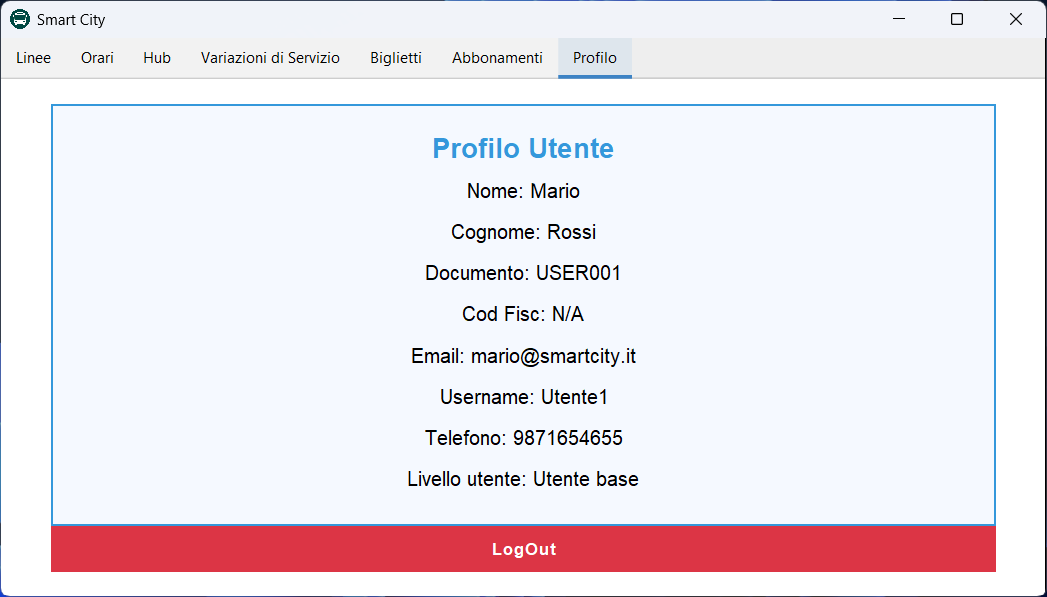
\includegraphics[width=0.6\textwidth]{app/Profilo}
  \caption{Visualizzazione del Profilo}
\end{figure}


\section{Funzionalità di base}
Quando si entra nell'applicativo, è possibile accedere alle funzionalità di base disponibili \underline{per tutti i tipi di utente} (anche per i non loggati) tramite la barra di navigazione posta sulla parte superiore della finestra. \\
\begin{figure}[H]
  \centering
  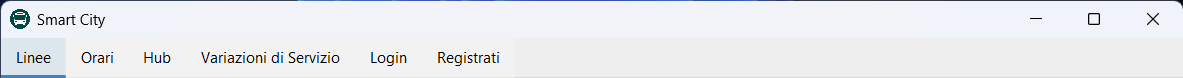
\includegraphics[width=1.0\textwidth]{app/NavbarNonLoggato}
  \caption{Barra di navigazione per utenti non loggati}
\end{figure}

\begin{itemize}
    \item \textbf{Linee}: in questa scheda vengono visualizzate \textbf{tutte le linee} (sia ordinarie che straordinarie) \textbf{attive} al momento della consultazione della compagnia, in particolare: il codice della linea, il mezzo che la effettuerà, la fermata di partenza e arrivo, il tempo di percorrenza (in minuti) e un pulsante che aprirà in automatico la scheda \texttt{Orari} con la linea scelta.
\begin{figure}[H]
  \centering
  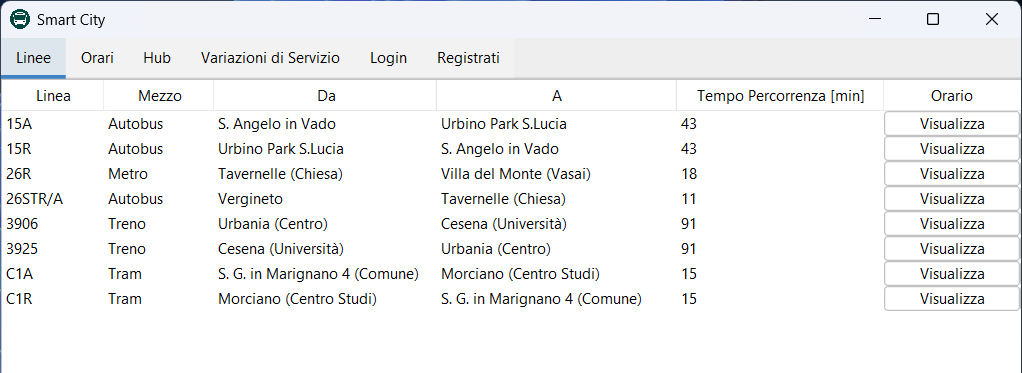
\includegraphics[width=0.7\textwidth]{app/Linee}
  \caption{Lista delle linee attive}
\end{figure}
    \item \textbf{Orari}: selezionando la linea di nostro interesse (scegliendola dal menù a tendina e cliccando il tasto "OK") verrà visualizzata nella zona sottostante la tabella con gli orari della linea selezionata. La tabella presenta nella prima colonna le fermate che compongono la linea (in ordine di percorrenza), mentre nelle colonne successive sono presenti gli orari per ogni fermata nel giorno della settimana di riferimento.
\begin{figure}[H]
  \centering
  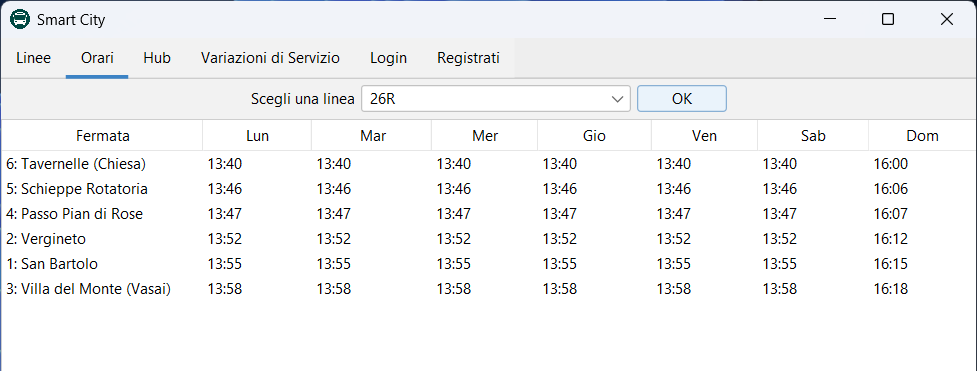
\includegraphics[width=0.7\textwidth]{app/Orari}
  \caption{Visualizzazione dell'orario dettagliato di una linea}
\end{figure}
    \item \textbf{Hub}: Vengono mostrati i vari hub con i loro dati (nome, indirizzo, eventuale fermata di riferimento, posti disponibili, ecc...). Se sono presenti più contenuti per un hub, questi vengono ripetuti.
    \item \textbf{Variazioni di servizio}: scegliendo una linea ordinaria dal menù a tendina, verranno mostrate le eventuali variazioni di servizio per la linea scelta, ovvero il motivo della manuntenzione, la data di inizio, la data di fine e una lista delle eventuali linee sostitutive.
\begin{figure}[H]
  \centering
  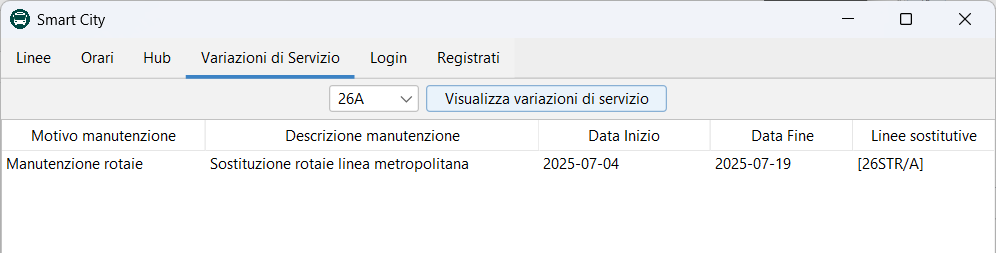
\includegraphics[width=0.8\textwidth]{app/VariazioniServizio}
  \caption{Visualizzazione delle variazioni di servizio per una linea}
\end{figure}
\end{itemize}


\section{Amministrativo}
Poiché agli utenti amministrativi è delegata la gestione di tutto il sistema di trasporto, sono gli utenti con il maggior numero di funzionalità disponibili.
\begin{figure}[H]
  \centering
  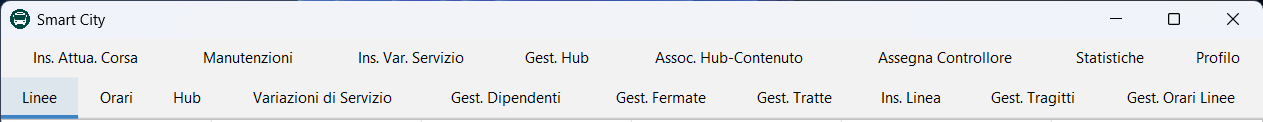
\includegraphics[width=1.0\textwidth]{app/NavbarAmministratore}
  \caption{Barra di navigazione per gli Amministrativi}
\end{figure}
\begin{itemize}
    \item \textbf{Gestione Dipendenti}: nel lato sinistro è possibile assegnare agli \texttt{Utente base} il ruolo di un dipendente, mentre nel lato destro è possibile declassare un dipendente a un utente base.
    \item \textbf{Gestione Fermate}: nel lato sinistro è possibile aggiungere una fermata, compilando i dati nelle caselle e premendo su Aggiungi Fermata. Nel lato destro è possibile rimuovere una fermata selezionandola dal menù a tendina.
    \item \textbf{Gestione Tratte}: nel lato sinistro è possibile aggiungere una tratta selezionando dai menu a tendina le fermate di partenza e arrivo e inserendo il tempo di percorrenza. Se la fermata di partenza è uguale a quella di arrivo, viene impedita l'aggiunta. Nel lato destro è possibile rimuovere una tratta.
    \item \textbf{Inserimento linea}: nel lato sinistro è possibile inserire i dati di una linea, mentre sul lato destro è possibile comporne il tragitto aggiungendo varie tratte (che devono già essere state inserite tramite l'apposita funzione). Per eliminare una tratta inserita si deve premere su \textit{Elimina ultima tratta}, sul lato sinistro. Compilati i dati di una linea e inserite le tratte, si potrà aggiungere la linea con il pulsante \textit{Aggiungi linea}. Da notare che mano a mano che si aggiungono le tratte, il menù a tendina suggerisce solo quelle che sono compatibili con la tratta precedente (fermata di partenza coincidente con la fermata di arrivo della tratta precedente).
    \item \textbf{Gestione tragitti}: nel lato sinistro è possibile aggiungere una tratta alla fine della linea selezionandola dal menù a tendina. Nel lato destro è possibile rimuovere l'ultima tratta assegnata a una linea.
    \item \textbf{Gestione orari linee}: nel lato sinistro è possibile aggiungere un orario di partenza settimanale ad una linea. Vanno selezionati la linea, l'ora di partenza e uno o più giorni di validità. Nel caso vengano spuntati più giorni, questi vengono tutti aggiunti all'orario con la medesima ora di partenza. Nel lato destro, data una linea, è possibile eliminarne un orario.
    \item \textbf{Inserimento attuazione corsa}: viene registrata l'effettiva attuazione di una corsa, specificando il giorno, la linea, l'orario di partenza, il mezzo e l'autista. Con questa funzionalità, viene automaticamente aggiunta la linea all'\textbf{orario di lavoro} di un \texttt{Autista}. Data la presenza di vari vincoli da rispettare, l'inserimento è guidato. Va inizialmente scelta la data di interesse, così che saranno proposte solo le linee attive e che hanno un orario disponibile per quel giorno. Una volta scelta la linea, è possibile scegliere l'orario desiderato e il mezzo che dovrà svolgere la corsa. Infine viene assegnato il turno di lavoro a un certo autista.
\begin{figure}[H]
  \centering
  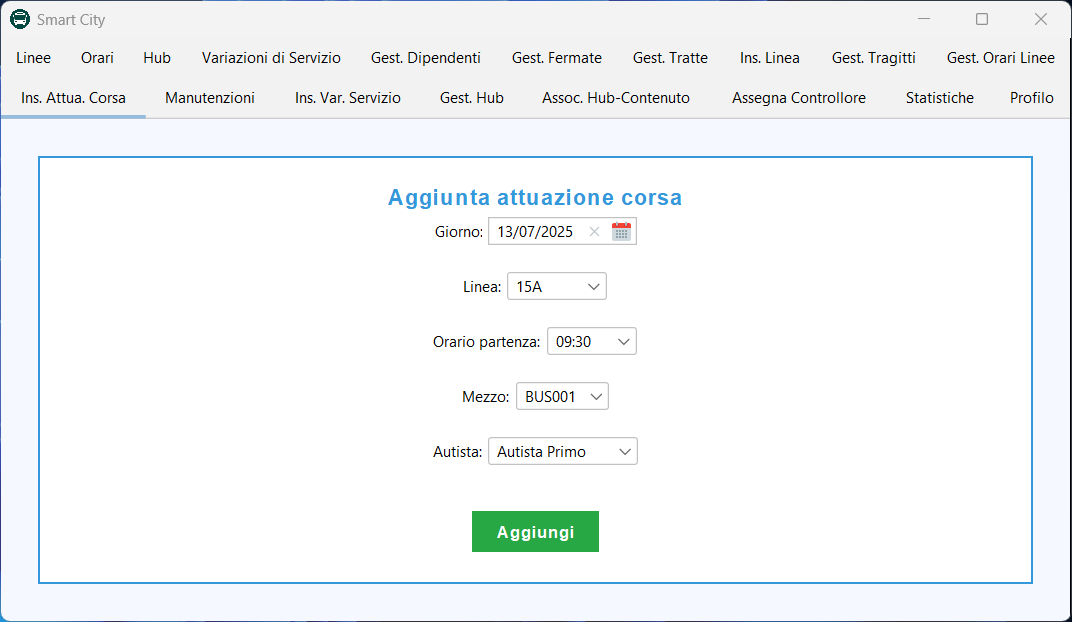
\includegraphics[width=0.7\textwidth]{app/AttuazioneCorsa}
\end{figure}
    \item \textbf{Manutenzioni}: in questa scheda sarà possibile gestire le manutenzioni di mezzi e linee ordinarie; si presenta con un menù a tendina dal quale effettuare la scelta mezzi / linee. Una volta scelto si aprirà una pagina, che sarà uguale per entrambe, con a sinistra (pannello blu) la possibilià di aggiungere manutenzioni, mentre a destra (pannello rosso) la possibilità di rimuovere le manutenzioni. Per aggiungere le manutenzioni verranno richiesti vari dati: la linea (o il mezzo), la data di inizio e fine, un nome, una descrizione e, se il lavoro è stato svolto da un'azienda esterna, la partita iva.
    \item \textbf{Inserimento variazione di servizio}: data una manuntenzione relativa a una linea è possibile aggiungere una linea sostitutiva. La manuntenzione e la linea da sostituire devono essere già state aggiunte nelle loro schede. Le linee sostitute possono essere solo straordinarie.
    \item \textbf{Gestione hub}: nel lato sinistro è possibile aggiungere un hub mobilità. Eventualmente si può anche aggiungere una fermata tra quelle presenti nel menu a tendina. In rimozione hub si possono rimuovere degli hub già inseriti nel sistema.
    \item \textbf{Associazione Hub-Contenuto}: nel lato sinistro è possibile associare a un hub un contenuto (macchine elettriche, bici scooter, ecc...) e il numero di posti massimi relativi ad esso. Gli hub devono essere già inseriti nel sistema in \textit{Gestione hub}. Nel lato destro è possibile rimuovere un'associazione.
    \item \textbf{Assegna controllore}: viene effettuata l'assegnazione di una corsa a un \texttt{Controllore}, componendo così il suo \textbf{orario di lavoro}.
    \item \textbf{Statistiche}: in questa scheda sono presenti diverse statistiche riguardanti il sistema. Si seleziona il tipo di statistica da visualizzare in un menu a tendina e si preme \textit{OK} per ricevere il risultato. Per alcune operazioni è necessario aggiungere ulteriori informazioni: si devono compilare i campi e premere il relativo pulsante per ottenere la statistica.
\begin{figure}[H]
  \centering
  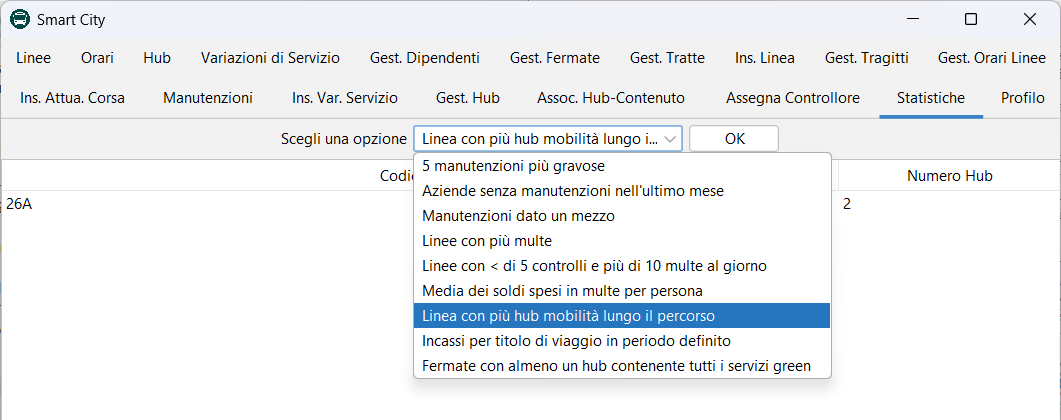
\includegraphics[width=0.8\textwidth]{app/Statistiche}
  \caption{Lista delle statistiche disponibili}
\end{figure}
\end{itemize}

\section{Autista}
\begin{figure}[H]
  \centering
  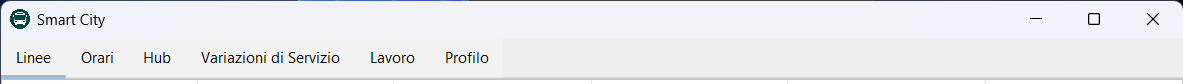
\includegraphics[width=1.0\textwidth]{app/NavbarAutista}
  \caption{Barra di navigazione per gli Autisti}
\end{figure}
\begin{itemize}
    \item \textbf{Lavoro}: in questa pagina l'autista può visualizzare il proprio orario di lavoro. La tabella è organizzata in modo da avere nella prima colonna la data, seguita da il codice della linea, l'orario di partenza e arrivo della linea che gli è stata assegnata, il mezzo e un tasto con il quale potrà visualizzare gli orari e le fermate della linea. Gli orari visualizzati sono quelli inseriti dagli utenti \texttt{Amministrativi} nell'\texttt{Attuazione corsa}.
\begin{figure}[H]
  \centering
  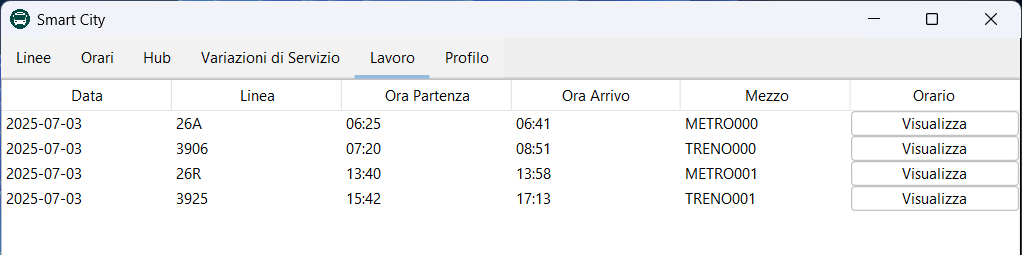
\includegraphics[width=0.8\textwidth]{app/LavoroAutista}
  \caption{Orario di lavoro di un Autista}
\end{figure}
\end{itemize}

\section{Controllore}
\begin{figure}[H]
  \centering
  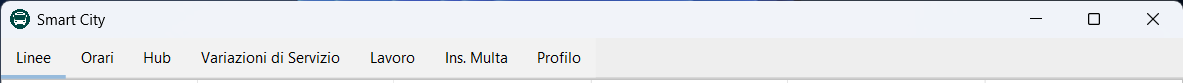
\includegraphics[width=1.0\textwidth]{app/NavbarControllore}
  \caption{Barra di navigazione per i Controllori}
\end{figure}
\begin{itemize}
    \item \textbf{Lavoro}: vengono visualizzate tutte le linee su cui il controllore dovrà eseguire i controlli. Gli orari visualizzati sono quelli aggiunti dagli \texttt{Amministrativi} nell'apposita scheda \texttt{Assegna controllore}.
\begin{figure}[H]
  \centering
  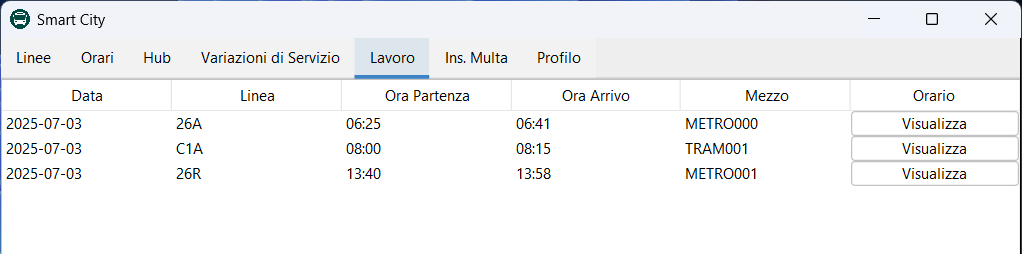
\includegraphics[width=0.8\textwidth]{app/LavoroControllore}
  \caption{Orario di lavoro di un Controllore}
\end{figure}
    \item \textbf{Inserimento Multa}: nel pannello di destra il controllore puà emettere una multa per una persona. Nel caso la persona non sia già registrata nel sistema, il controllore può inserirne i dati nel pannello di sinistra.
\begin{figure}[H]
  \centering
  \includegraphics[width=0.8\textwidth]{app/InserimentoMulta}
  \caption{Pannello per l'emissione di una multa}
\end{figure}
\end{itemize}


\section{Utente}
\begin{figure}[H]
  \centering
  \includegraphics[width=1.0\textwidth]{app/NavbarUtente}
  \caption{Barra di navigazione per gli utenti base}
\end{figure}
\begin{itemize}
    \item \textbf{Biglietti}: nella parte superiore è presente un menù a tendina per selezionare se vogliamo acquistare o convalidare un biglietto. Nel caso dell'acquisto avremo un'altro menù dal quale potremo scegliere la durata del biglietto, un pulsante per confermare l'acquisto e uno per visualizzare le tariffe.\\ Nella pagina di convalida troveremo invece due menù: uno per segliere il codice del biglietto che vogliamo convalidare, nell'altro la corsa sulla quale vogliamo convalidare il nostro biglietto.
    \item \textbf{Abbonamenti}: in questa pagina abbiamo il primo menù per scegliere la durata del nostro abbonamento, subito sotto dovremmo scegliere la data di inizio validità dell'abbonamento, poi troveremo due bottoni: acquista e visualizza tariffe.
\begin{figure}[H]
  \centering
  \includegraphics[width=0.7\textwidth]{app/AcquistoAbbonamenti}
  \caption{Pannello per l'acquisto di un abbonamento}
\end{figure}
\end{itemize}

\end{document}
